\section*{Rio De Janeiro}
Nyttårsaften årskifte 2014 og 2015 ble tradisjonen tro tilbrakt i
fuktig lag på Hovden. Tradisjonen tro ble det også lite søvn. Neste
dag tilbrakte jeg natten hos en søte snelle som hadde gjort høsten
min i Kristiansand verdt bryet. Needles to say, det var ikke noe
særlig søvn den natten heller. Følgende satt jeg meg 2.Januar på et
fly til Brazil og sov frem til 10 minutt før landing. 
En av grunnene til at jeg valgte å ta pause fra studiet dette året var
at alle kameratene mine dro på utveksling. Noe som betaler seg to
ganger. Ikke bare er det helt dødt i Trondheim, men det er også mange
du kan besøke ute i den store verden!\#Gratisstedåbo Følgende er jeg
klar for 
å sjekke inn i leiligheten til tre kompiser på Copacobana.
Fire dager før hadde jeg fått adressen og jeg var fast bestemt på å ta
meg frem på egenhånd. Helst uten de hadde noen anelelse om når jeg
kom. Overralskelsesoppmøte er undervurdert. Adressen hadde jeg skrevet
ned og sidemannen min på flyet lærte meg å uttale ``Rua sa Fereirah'' rett før
landing.Selvsikkert satt jeg meg inn i taxien og sa ``rua sa fereirah, por
favor''. Etter 4 forsøk ga jeg ham bare lappen.\\ 
\begin{wrapfigure}{r}{0.5\textwidth}
	\begin{center}
		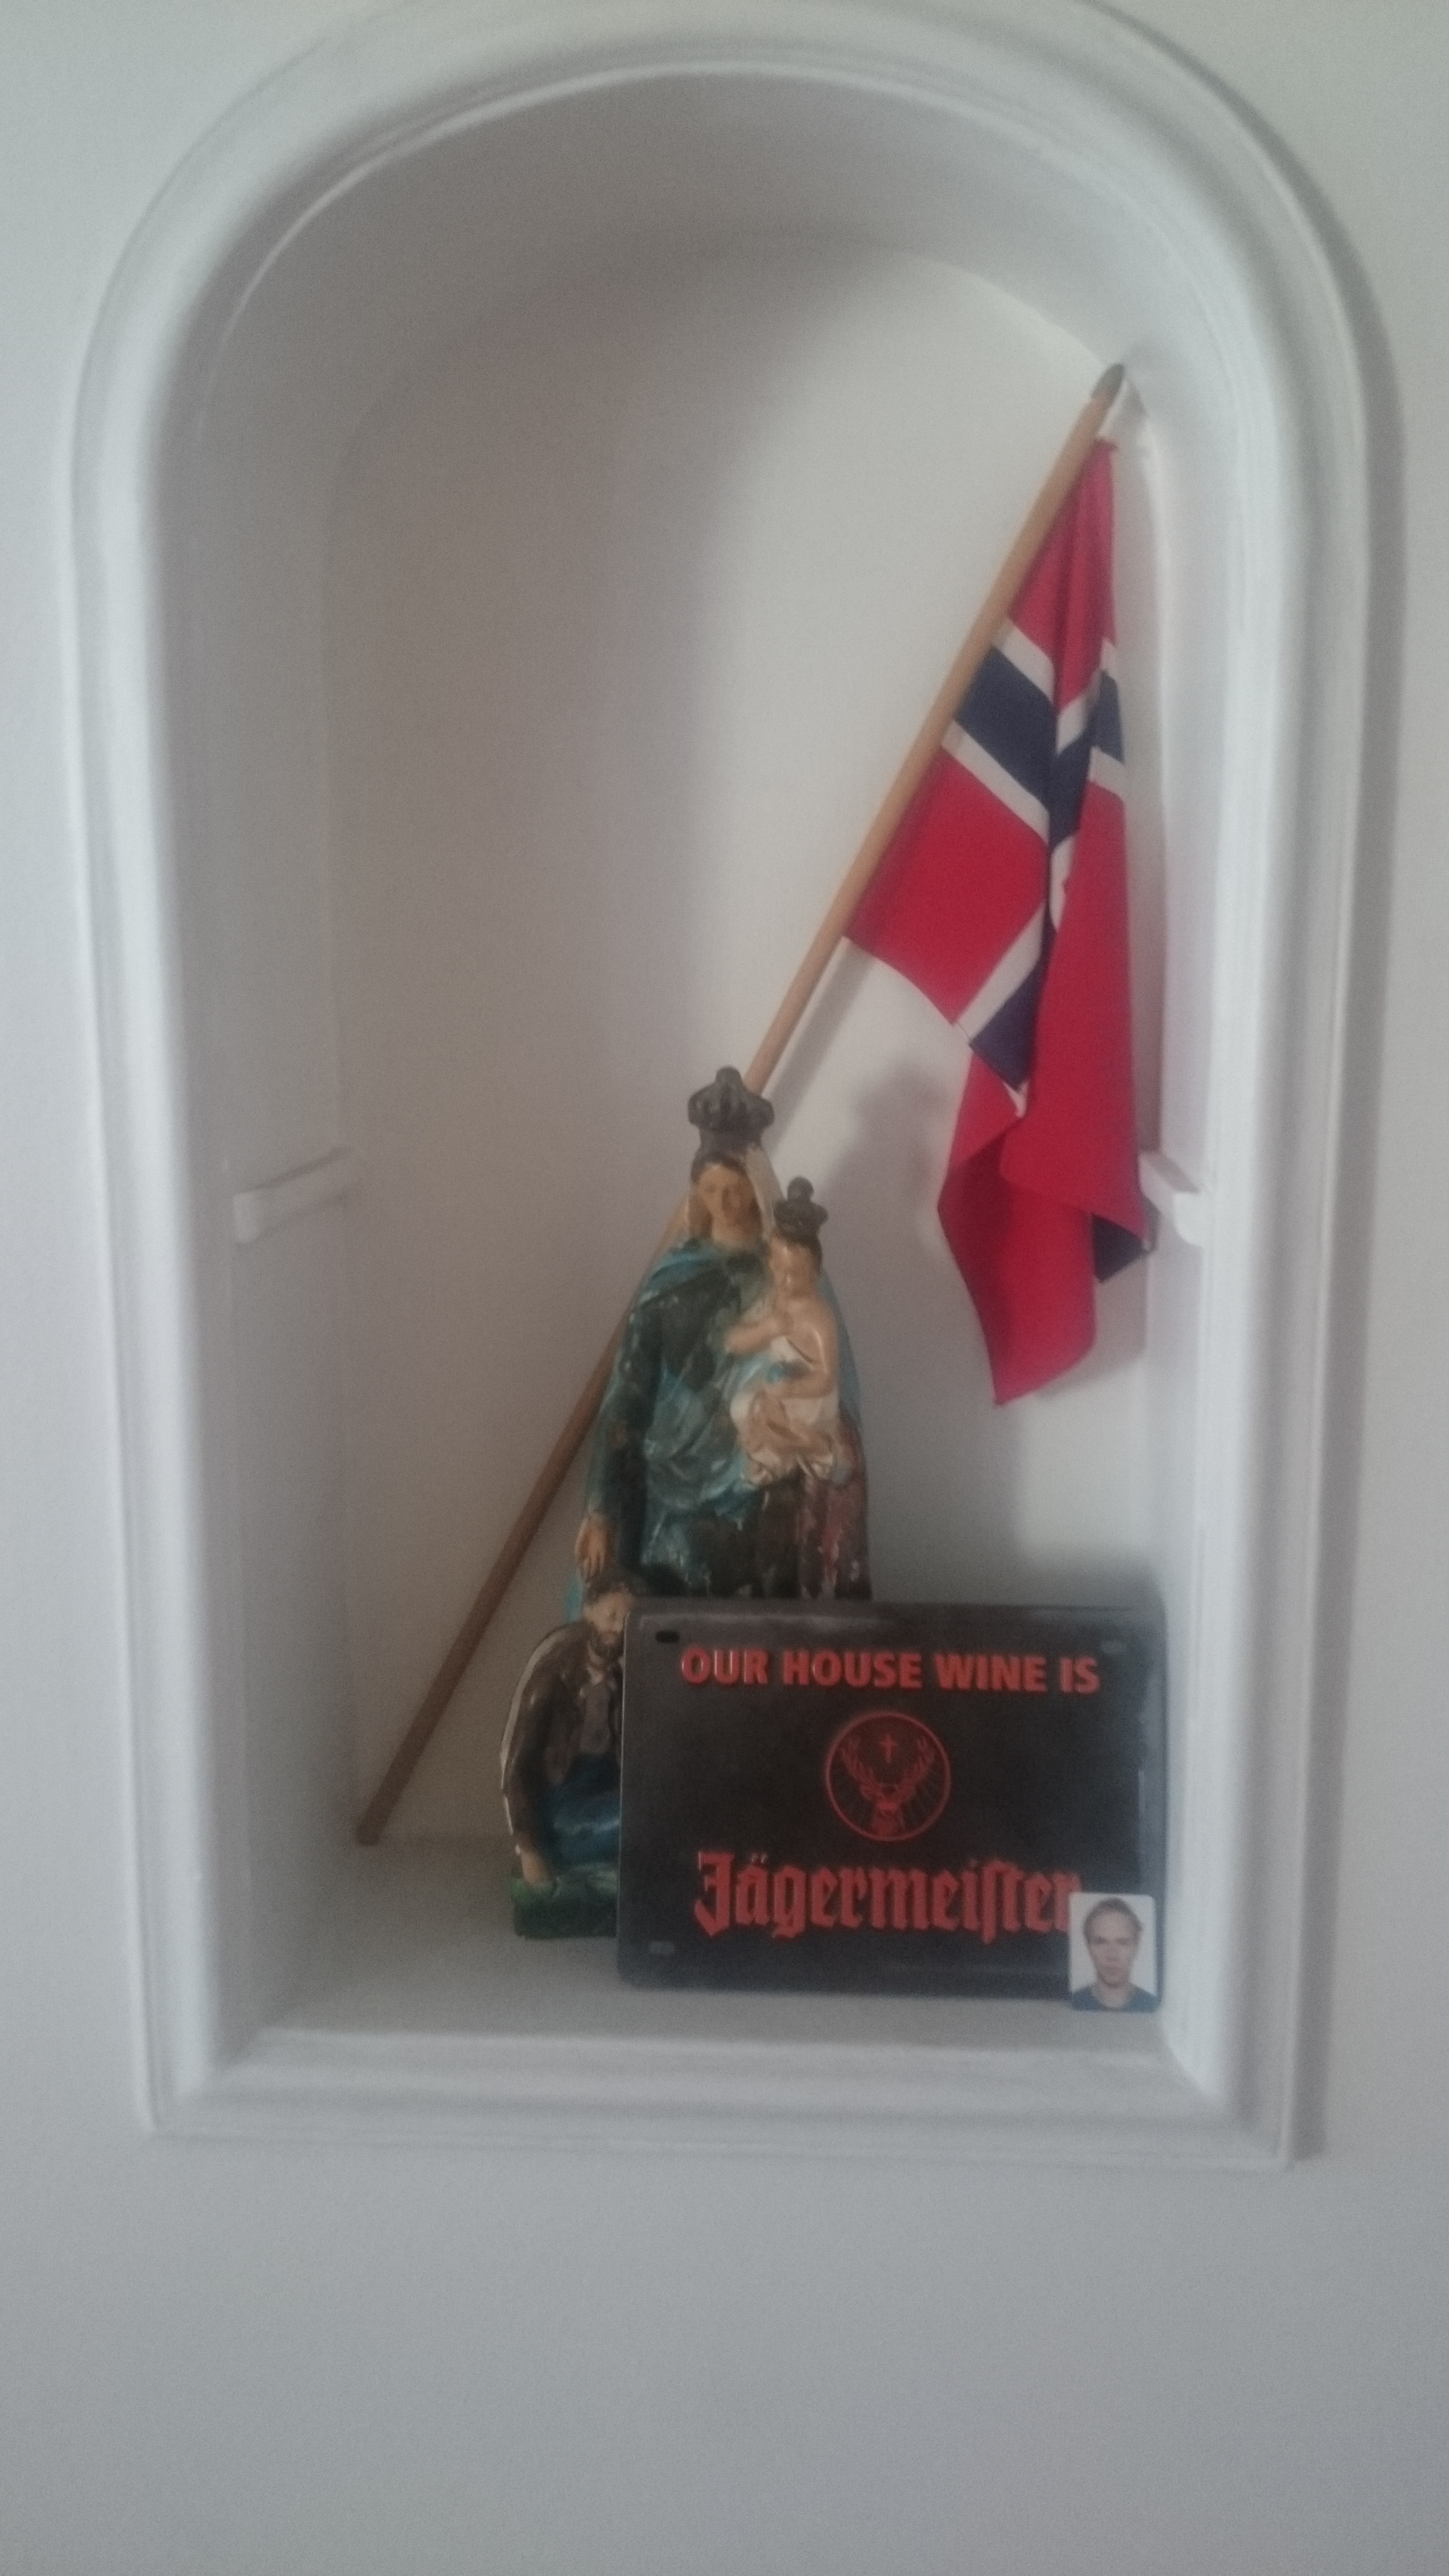
\includegraphics[width=0.35\textwidth]{slakteriet}
	\end{center}
	\caption{Slakteriet setter standarden}
\end{wrapfigure}
Jeg kom frem til et leilighetskompleks. Det var låst. Men heldigvis
satt det en mann innenfor som kunne låse opp. ``Griseflaks'', tenkte jeg.
Ikke før vi gikk ut igjen jeg forstod at dette var jobben hans. Ikke
rart han var litt gretten. Nøkler
er oppskrytt. Fant senere ut at dette er en ganske variert jobb i Rio.
Finnes karer som sin eneste dagsoppgave er å trykke på etasjen i
heisen for deg. 

Heldigvis var det rett leilighet. Og jeg fikk den best tenkelige
velkomts; et par
bjørneklemmer, lystig lag og en kald pils. Senere den kveldent stakk
vi på byen. Og det eneste jeg har planer om å ha på papir fra den
kvelden er at utestedet kalte seg noe så frekt som ``la-Passion''.
\clearpage

\subsection*{Om kulturkræsj}
\begin{figure}[h]
	\centering
	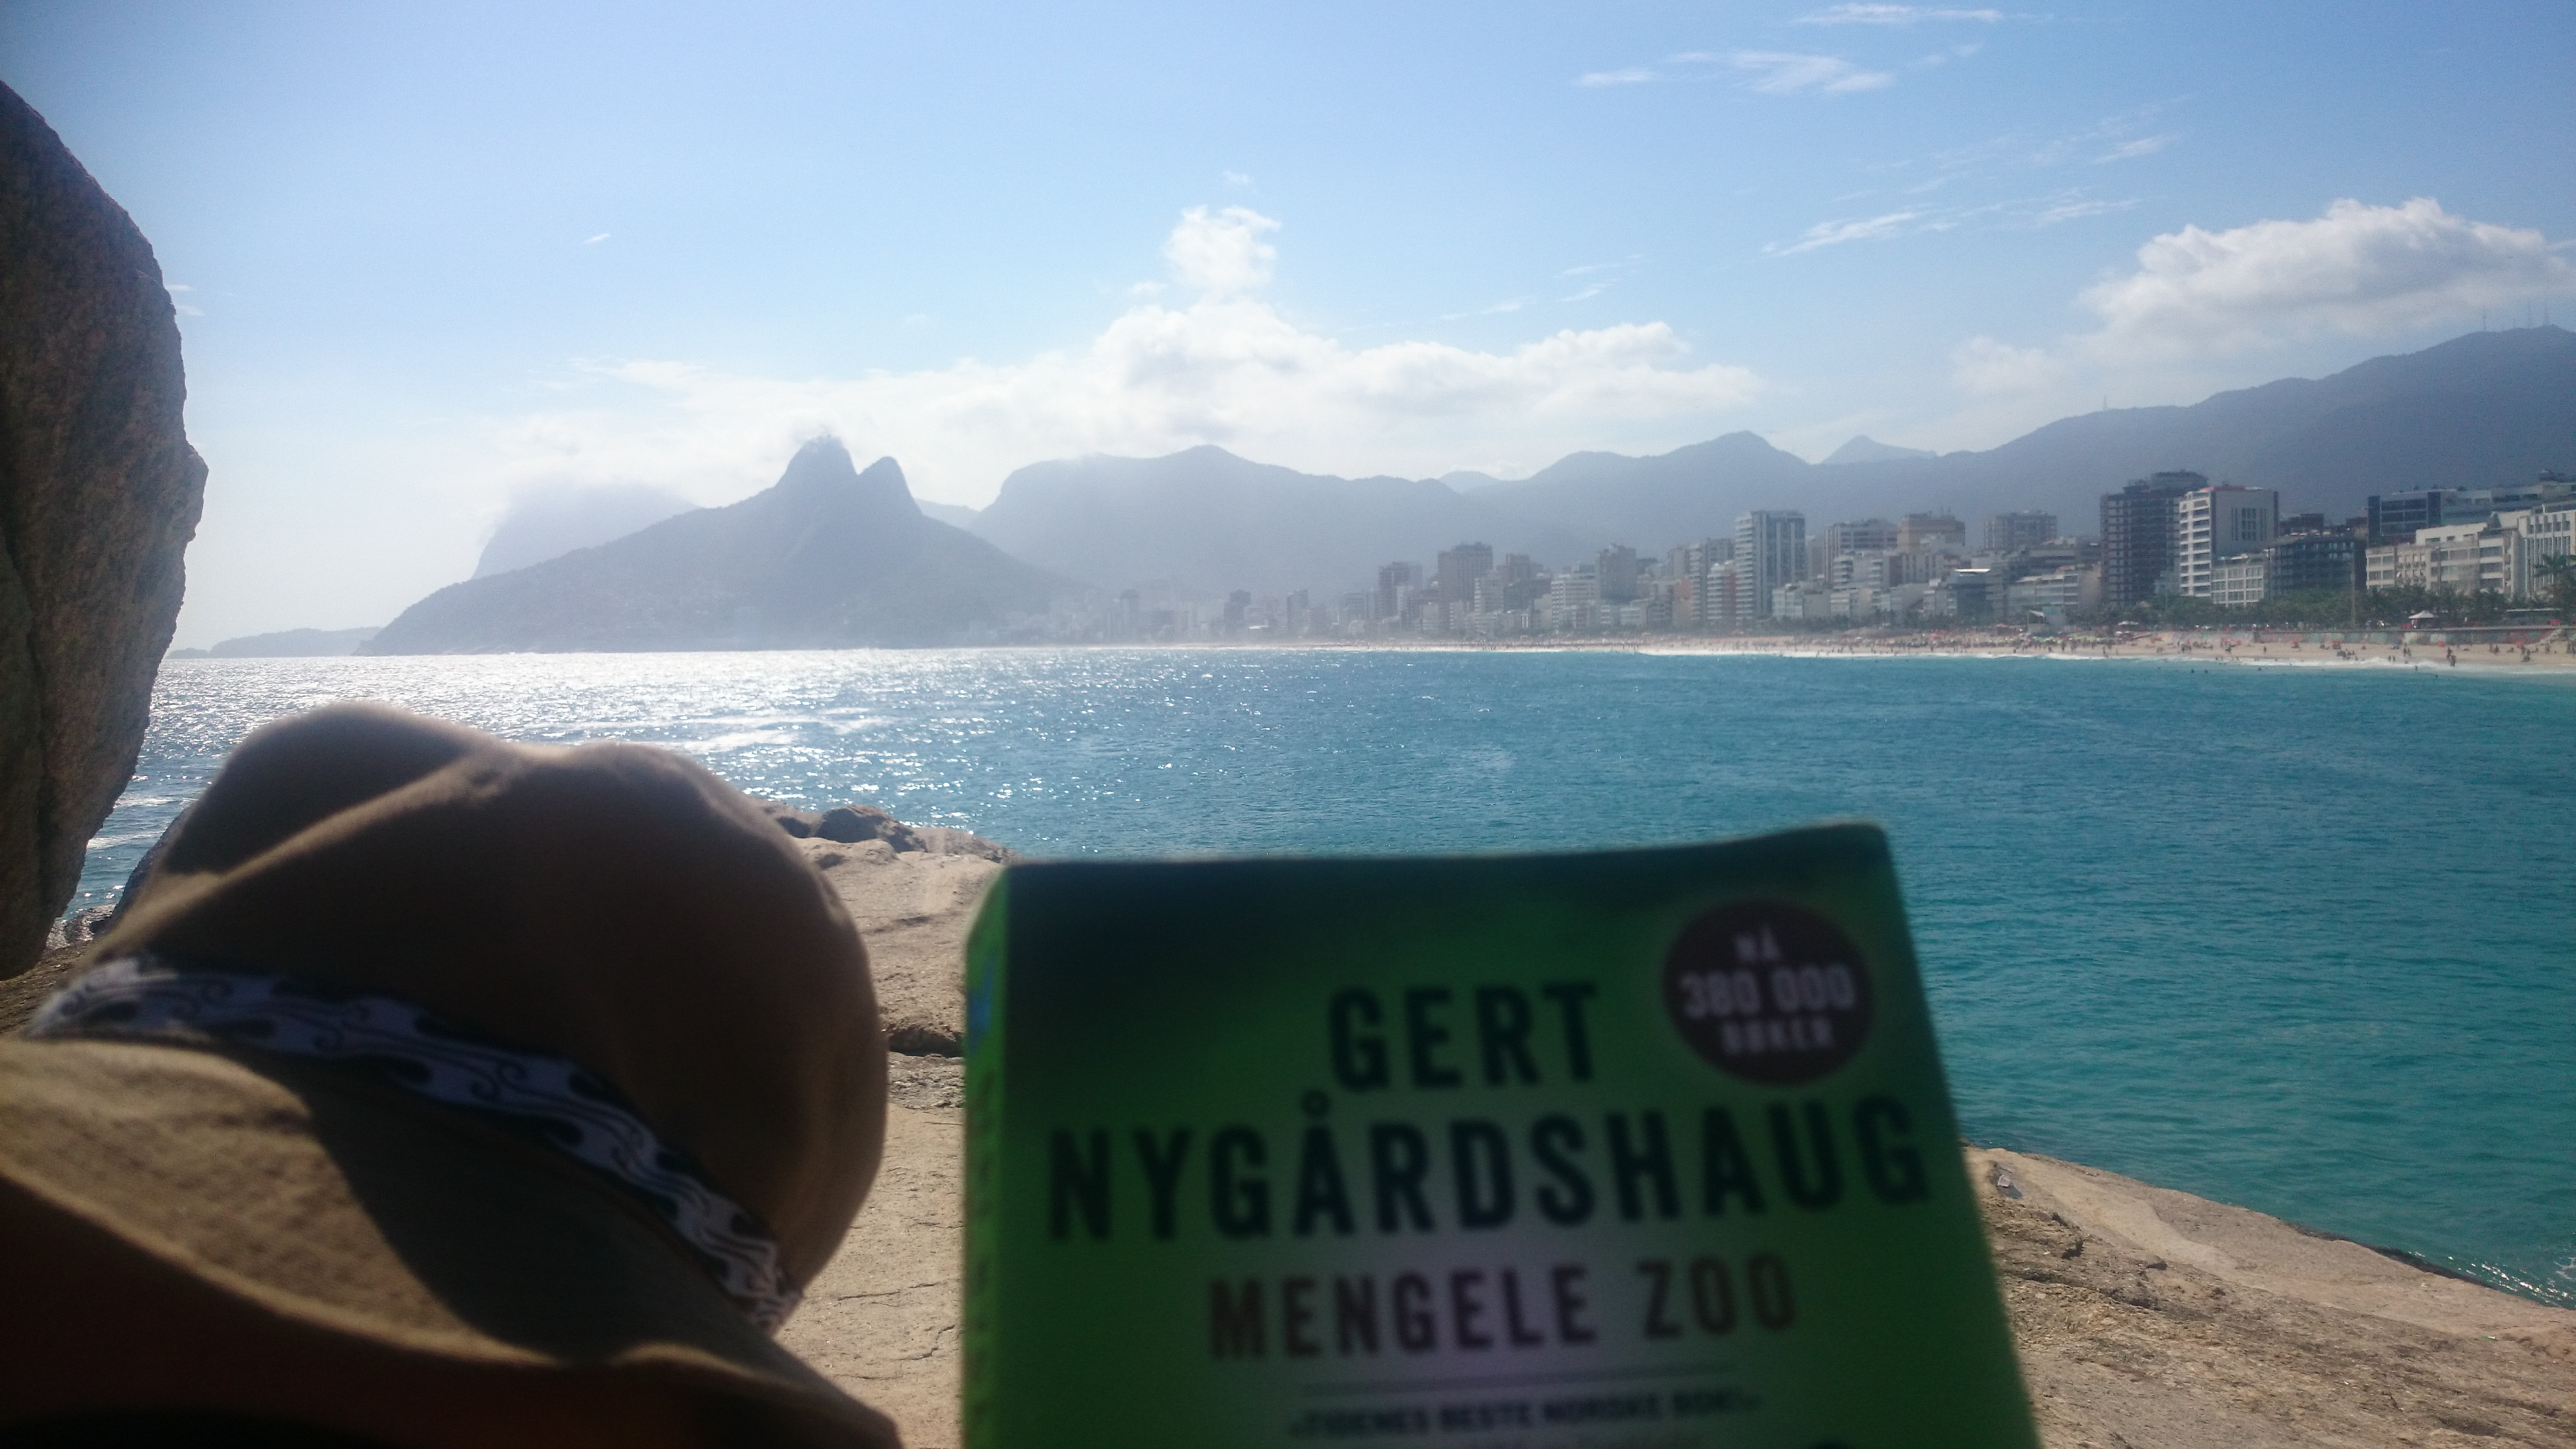
\includegraphics[width=\textwidth]{mengelezoo}
	\caption{Ipanema og lokalhistorie}
\label{fig:mengelezoo}

\end{figure}

Det er visse uttrykk man aldri vil høre i Brasil.
\begin{dialogue}
	\item ``Har noe sett flisen min?''\\
	\item ``Vi tar bussen!''\\
	\item ``Det blir godt med et glass melk''\\
	\item ``Neitakk, det er for tidlig med Carpirinha''\\	
\end{dialogue}
Og Viktigst av alle:\\
\begin{dialogue}
	\item ``Jeg tar bare en svipptur på butikken''
\end{dialogue}
Det finnes ikke noe som heter ``en-svipptur-på-butikken'' i Rio\ldots Å dra på butikken er
et dagsprosjekt. Minst.  Og det er egentlig bare en grunn til dette.
Brasilianere er trege! Ikke sørlending trege, de er 1.nyttårsdag
trege. De kjemper seg gjennom sirup. Å kjøpe et par varer på butikken
tar minst tre kvarter. For en over gjennomsnittet utålmodig kar rett
fra Norge var dette en utfordring. Så der var de et stort minuspoeng.
Heldigvis er det andre ting som trekker opp med Brasilianere. En av
dem er den totale mangelen av janteloven. Om man vil smøre seg inn i
sololje og løpe i baris langs den mest folksomme stranda er det ikke
bare akseptert, det er oppfordret!. Det de derimot syntes er rart er
hvorfor vi gringoer ligger på stranda. Gutter på stranda skal stå.
Ligge er noe jenter gjør. Gjerne med hoftefestet og enda bedre om man kommer rett fra en frekk styrkeøkt. Det er uvisst hvordan de klarer å stå rett opp
og ned i sola i flere timer. Min beste gjetning er at det faktisk
trekker. Det er motivasjon nok for de fleste!

Den første kvelden vi var ute klarte jeg meg med et par øl før vi jeg
traff puta. Så jeg hadde enda ikke blitt introdusert til Carpirinha.
Det er svært vanskelig å lage. Man trenger:

\begin{enumerate}
	\item Cashaca (sprit type billig type 40\%)
	\item lime 
	\item sukker
\end{enumerate}

Blandingsforholdet er tid-på-døgnet-basert og det kan egentlig ikke
gjøres feil. Ikke for det edle formålet i å bli å pære i det minste.
Og ærlig talt, det er den eneste legitime grunnen til å drikke
Cashaca. Alt annet ville vært selvskading. Jeg piner meg gjennom
vorspielet og kommer meg endelig til byen i håp om å få en øl, i det
minste noe brunt! Men den gang ei. Såvidt innenfor døren får jeg to
drinker av Kristoffer. Gjett hva. Yepsi. Carpirinha type 02:00
Blandingsforhold. Resten av turen spiste jeg ikke lime.
\clearpage
\subsection*{Enter fam. Maastad}
Etter en kort uke kommer Marius tilbake etter å ha vært familieguide i
Brazil. Da ble det fart på sakene!
Volleyball, surfing og ikke minst toppturer. Viktig å drive med litt
ærlig idrett. Dessverre dårlig med bilder fra volleyball og surfinga.
Mest fordi mobiler blir stjelt sekundet du legger dem fra deg. Vi
kompenserte heldigvis på toppturene! Verste bøygen var at Marius
skulle teste de nye skoene sine og fikk heftig gnagsår. Noe som var
veldig gøy ettersom vi skulle krysse Andesfjellene. 

\begin{figure}[H]
	\centering
	
	\noindent\makebox[\textwidth]{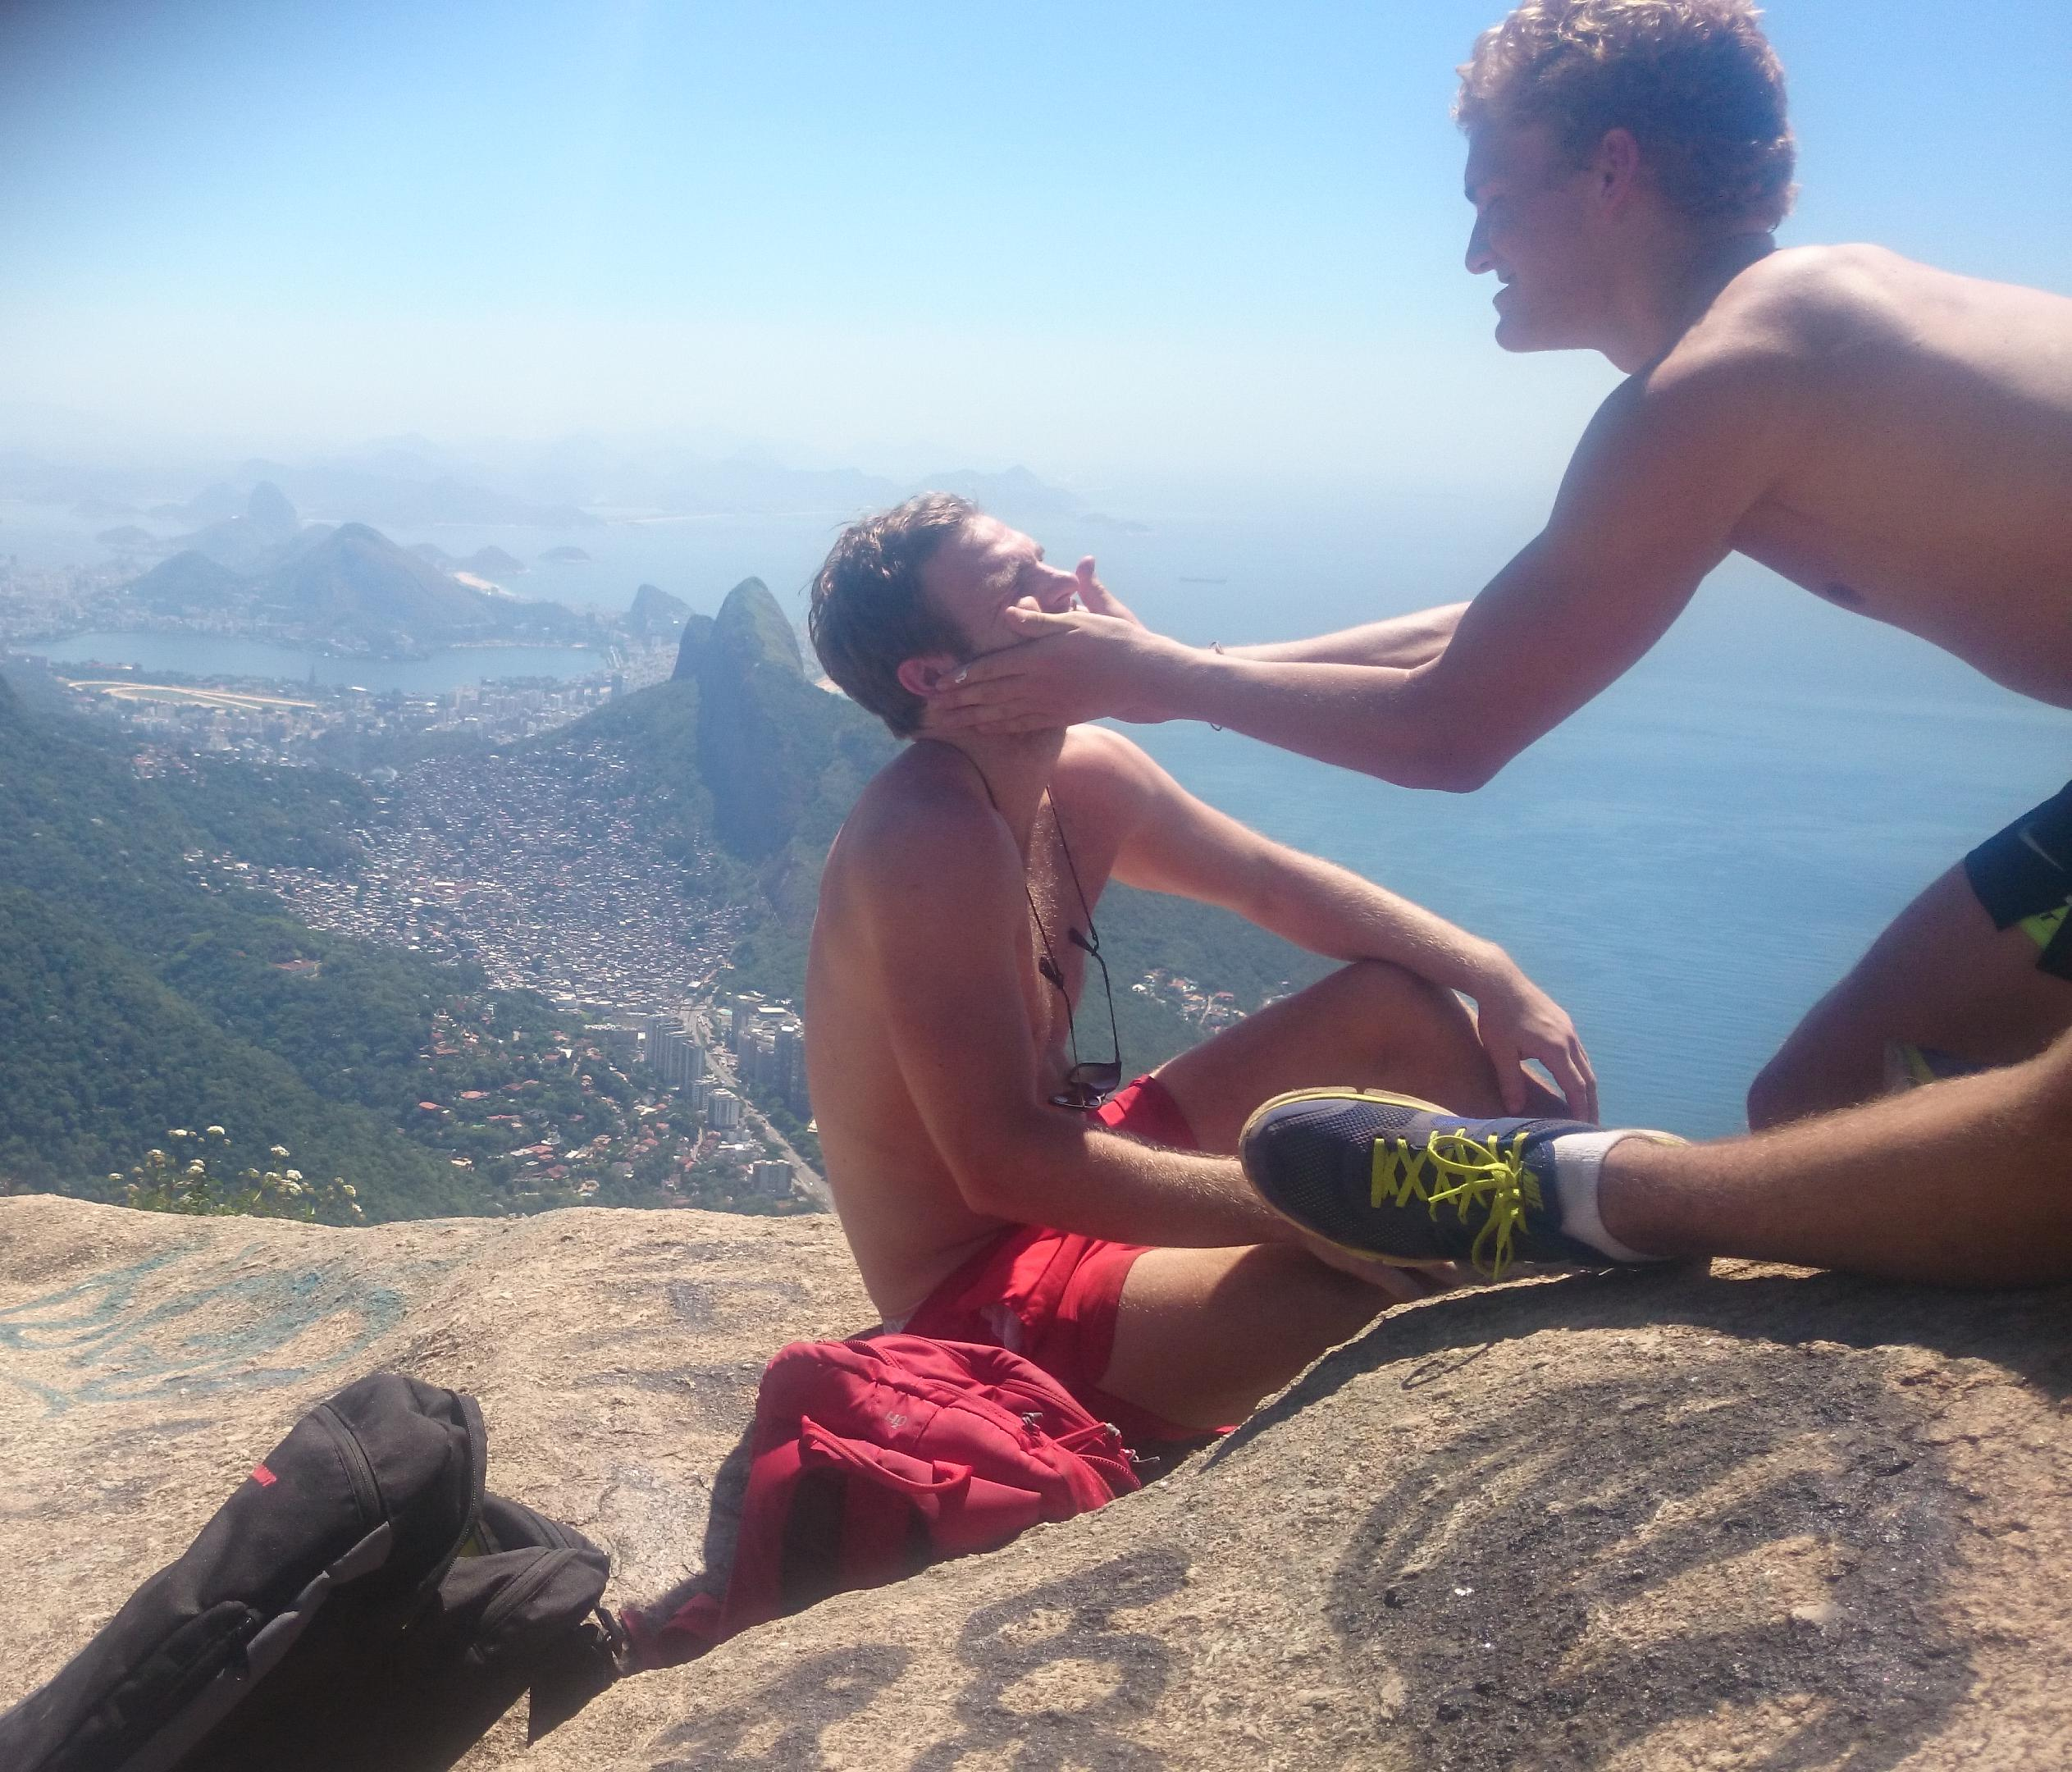
\includegraphics[width=\textwidth]{viktigaabrukeallsolkremen}}
	\caption{Viktig å bruke all solkremen}
\label{fig:predradegavea}
\end{figure}

\clearpage
\section*{Peru \\ {\footnotesize \textit{10--23 jan.}}}
\begin{figure}[!h]
	\centering
\noindent\makebox[\textwidth]{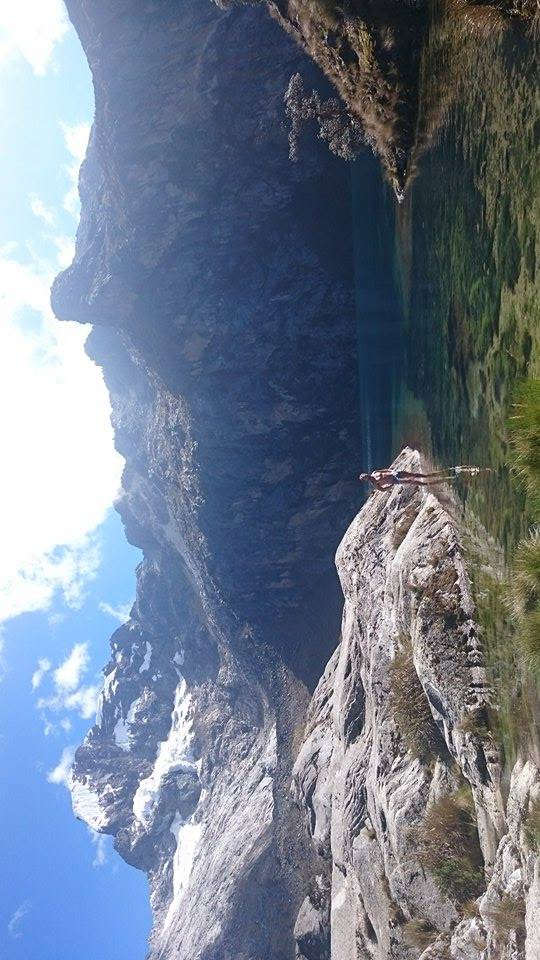
\includegraphics[width=\paperwidth]{coverphoto}}
	%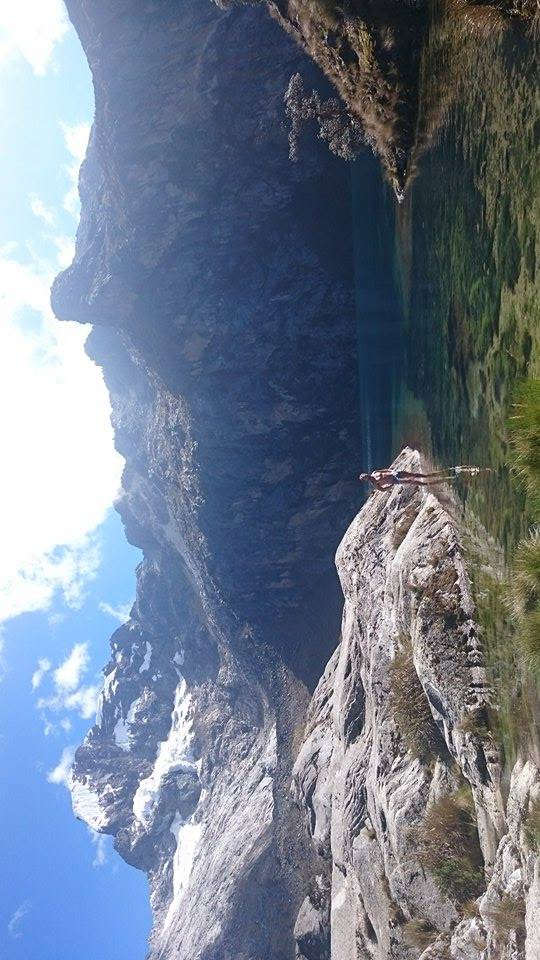
\includegraphics[width=\textwidth]{coverphoto}
	\caption{Rolig morgenbad}
\label{fig:coverphoto}
\end{figure}
\clearpage
\subsection*{City-life}



\begin{wrapfigure}{R}{0.45\textwidth}
	\begin{center}
		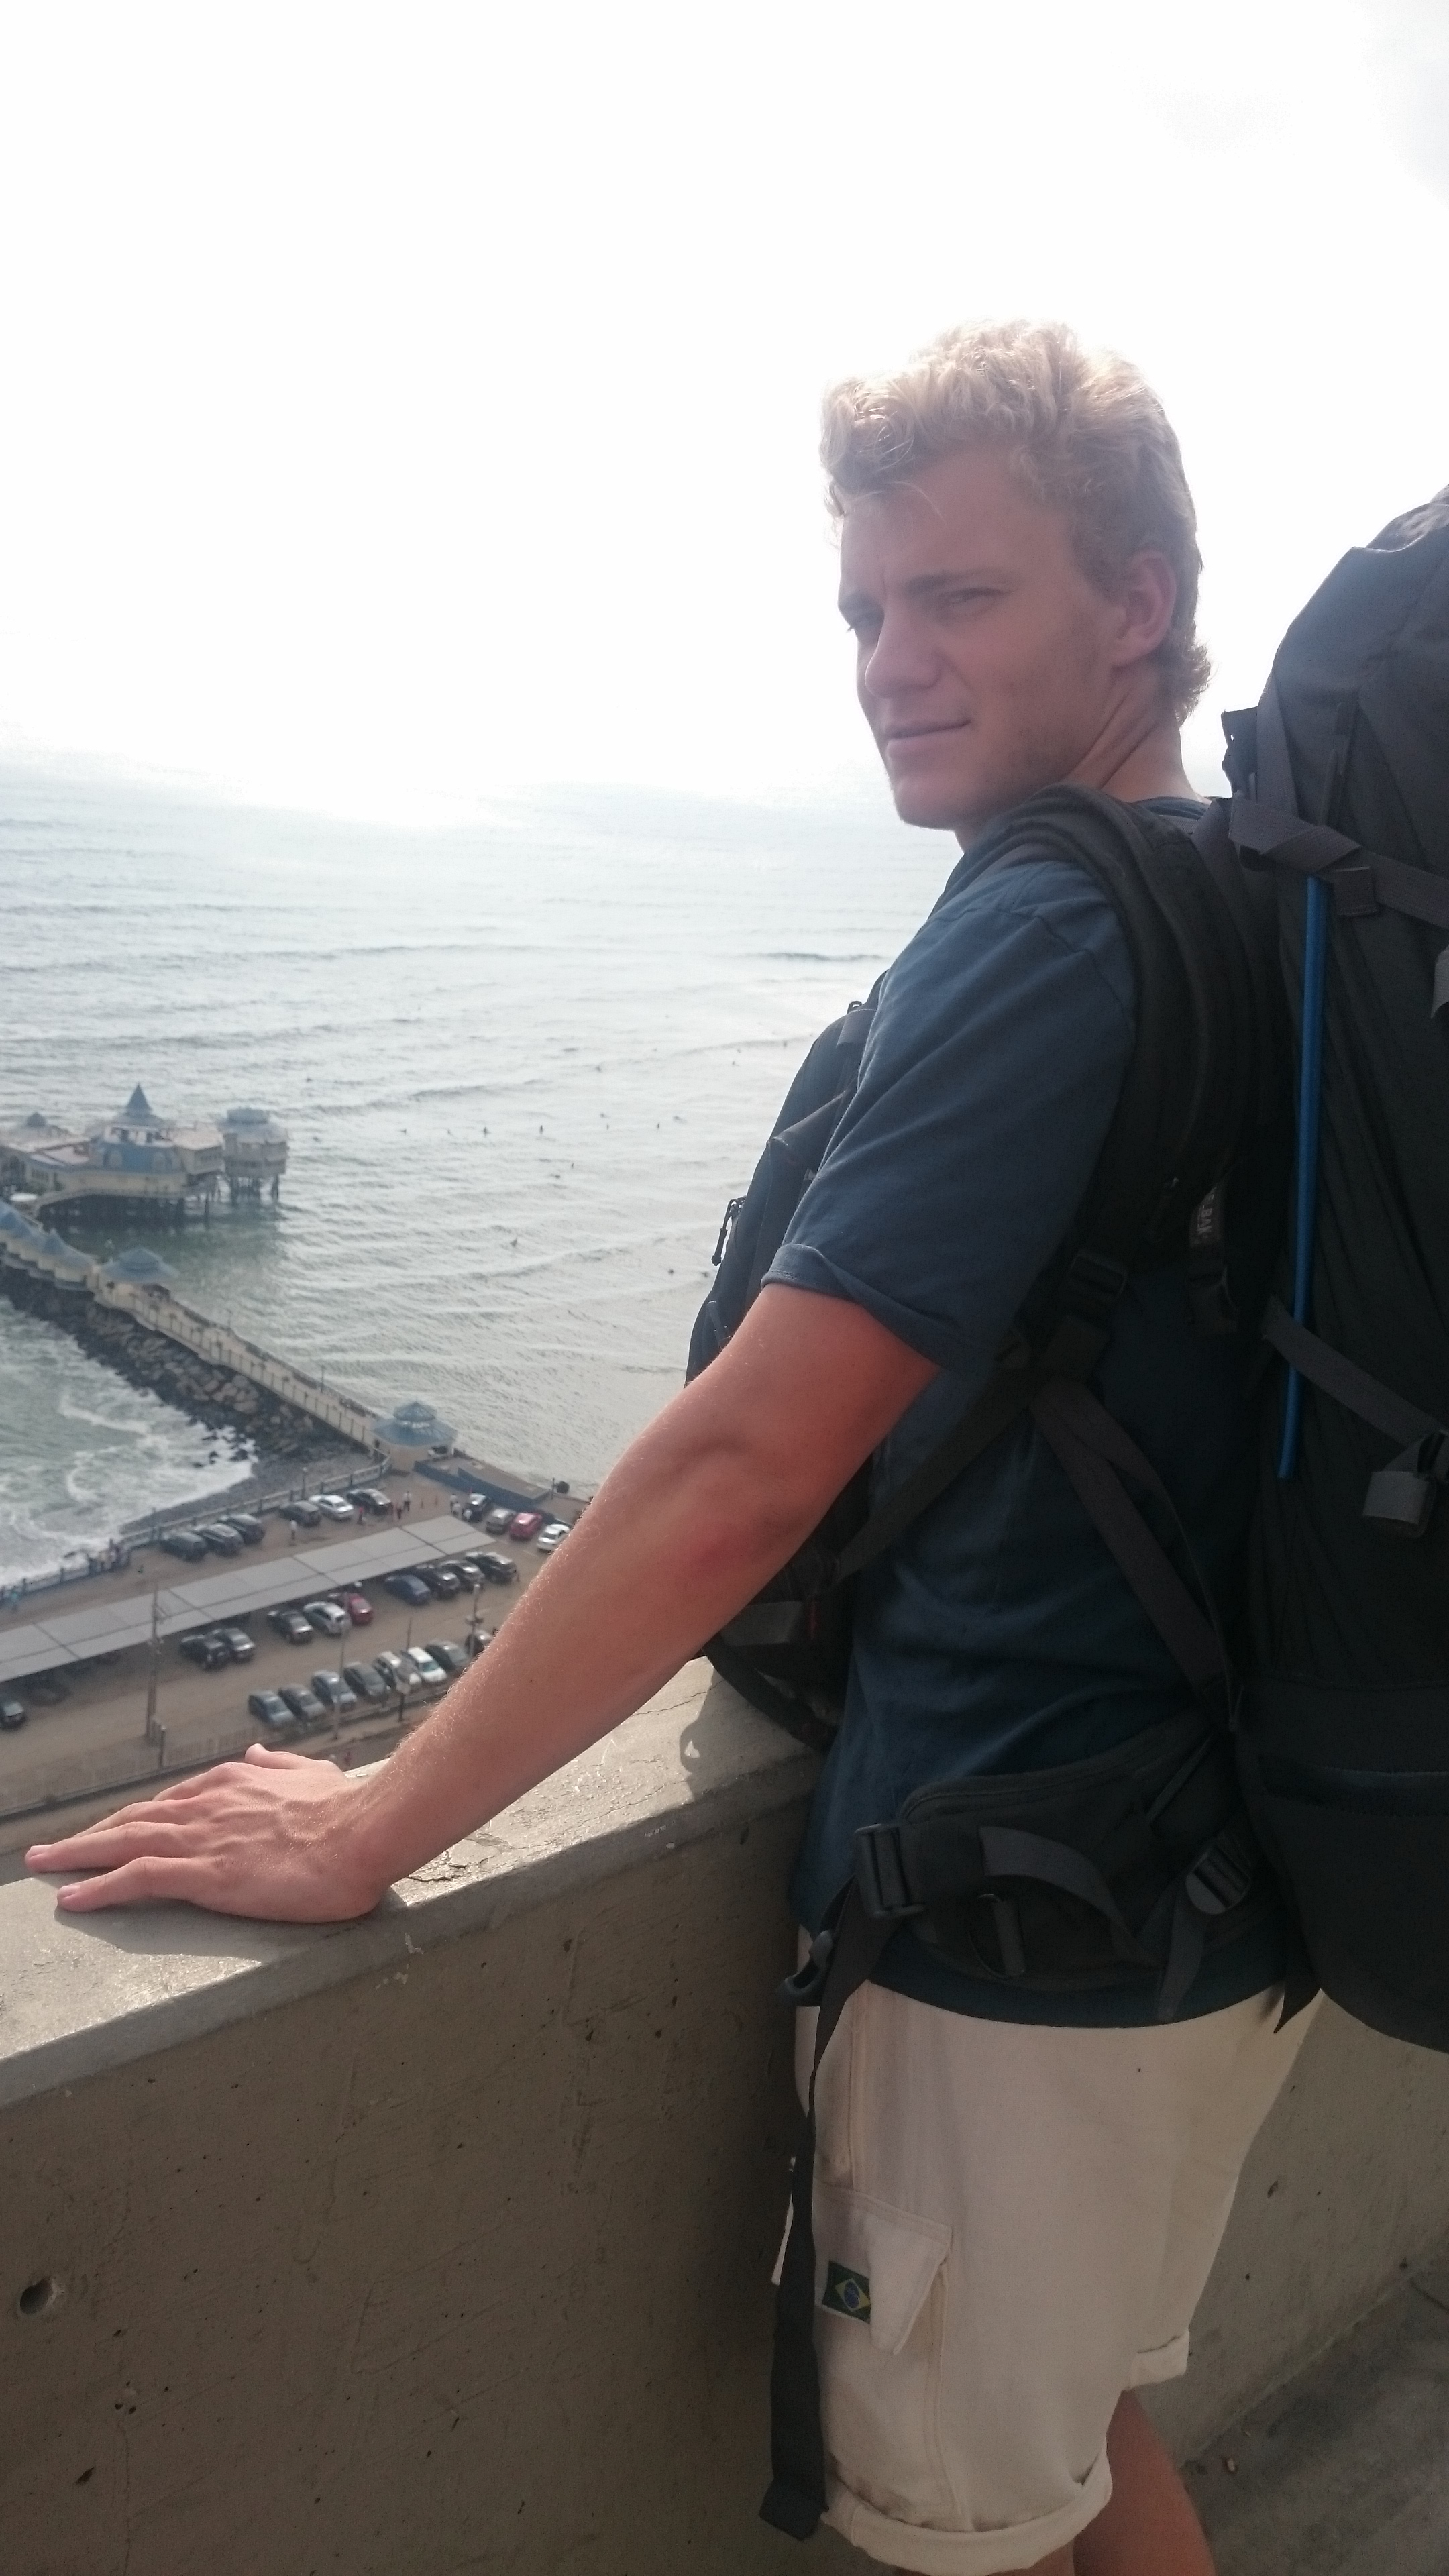
\includegraphics[width=0.48\textwidth]{stllehavet}
	\end{center}
	\caption{En halv klode med åpent hav}
\end{wrapfigure}
Eventyret til meg og Marius begynner med et smell da vi bestiller oss
et
rolig glass whiskey i overfarten til Peru. Det var fylt til
randen. Snakkes aldri.
Følgende var vi i lystig lag resten av flyturen og helt ut av
flyplassen. Det var vanskelig å ikke komme i godt humør gjennom
passkontrollen. Ja du hørte rett. Passkontrollen var god S. Men for å
forklare hvorfor må du vite et bar ting om Peru. For det først er ikke
Pruanere vant
til å se Europeere. For det andre ser de svært annerledes ut en oss.
De er generelt lave og alle har mørkt hår og øyne. Jeg
var så eksotisk at folk stoppet meg på gata for å ta bilder.
Platinablonde Maastek på 1.90 med øyne stjålet fra isbreen fikk folk
til å skli av stolen. Ok. Da har du bakgrunnsinformasjonen du
trenger. Det hadde imidlertid ikke vi! Fra min side var hendelseforeløpet slik: Marius
blir kalt frem til passkontrollen uten at damen bak skranken ser opp.
Når han er halveis mellom køen og skranken ser hun opp, sperrer opp
øyenene og gir beskjed om at han skal stoppe. Hun snur seg rundt
og finner frem telefonen. ``Fy-fabian'' tenkte jeg, skal de forhøre oss
nå? Det kommer sikker til å ta en halv evighet. Men den gang ei. Før
tanken helt rakk å formulere seg begynner Time after Time av Cyndi
Lauper å bråke ut fra telefonens høyttalere og gi gjenklang gjennom
lokalet. Marius blir så vinket frem til skranken. Der fortsetter hun
med å si:\\
\begin{dialogue}
	\item ``Du har så fine øyne'' 
\end{dialogue}\\
Før hun sender ham videre
gjennom. Marius gjør så den fatale og feilen i å se på meg. Jeg er nå
nesten på knærne ved bristepunktet til en latterkrampe. Ved øynekontakt
bristet det. For begge to. \\

At vi valgte å dra til Peru var litt på slump. Min fetter hadde nevnt
det var kult å gå i Andesfjellene og det skal være veldig lange
surfbreakes her. Det var tross dette et sjokk å lande i Lima og se at
vi er midt i en steinete ørken. Da med falleferdige bygninger, helst
uten tak. Vi sjekket inn på et hotell i et litt finere strøk og levde
litt city-life. Peru er eksportør av alpakka-ul. Og man kan si at vi
gikk litt bananas. Det ble mange skjerf og et par gensere. Men hadde
vært mye dyrere i Norge. Så vi sparte penger? Neida\ldots joda?
\clearpage

\subsubsection{Om hvordan kjøpe gaver}
Dette er ikke en ``om'' hva man skal kjøpe, men hvem. Alle
kan se en gjenstand å tenke:

\begin{dialogue}
	\item ``Den ville passet til (sett inn person) ''
\end{dialogue}

Men gitt dette ikke skjer, hvem burde man kjøpe til? Svaret er
enkelt. Man kjøper alltid gaver til de viktigste damene i sitt liv.\\

For å ta det første først: De setter mye mer pris på det! Gutter blir
glad for gaven. Jenter blir glad for gaven òg for at du tok deg tid
til å tenke på dem.\\

For det andre er det et oversiktlig antall personer. På hankjønn
siden har man Far, brødre, venner som er som brødre, videregående
venner, universitetsvenner, idrettssvenner, 
vente-på-kaffe-på-tyholt-venner, spilte-fotball-sammen-i-7.-venner. Er
håpløst. Med damer er det
annerledes. For meg er det mor, søster og evt. en romantisk
kompanjong. Minst 2, maks 3. Full kontroll. Det er sikkert en-
eller-annen kverulant her som mener han har en jentevenninne han har lyst
til å kjøpe en gave til. Du lurer ingen -- ikke deg selv en gang!\\

For det tredje kan du sannsynligvis kjøpe gave til alle i den samme
butikken. Man kan prøve så hardt man vil, men frøknene en tar med hjem
har det med å ha den samme stilen som de to som er der fra før. Kan
være dette kommer ut litt feil. Prøver bare å si at din standard for
damer
ikke nødvendigvis ble satt av deg selv! Det ble ikke min\ldots Og godt er det.\\


\subsection*{Treningsleir del 1}

%\begin{figure}[!h]
%	\centering
%	\includegraphics{<+file+>}
%	\caption{%\end{figure}

\begin{figure}[!h]
	\centering
|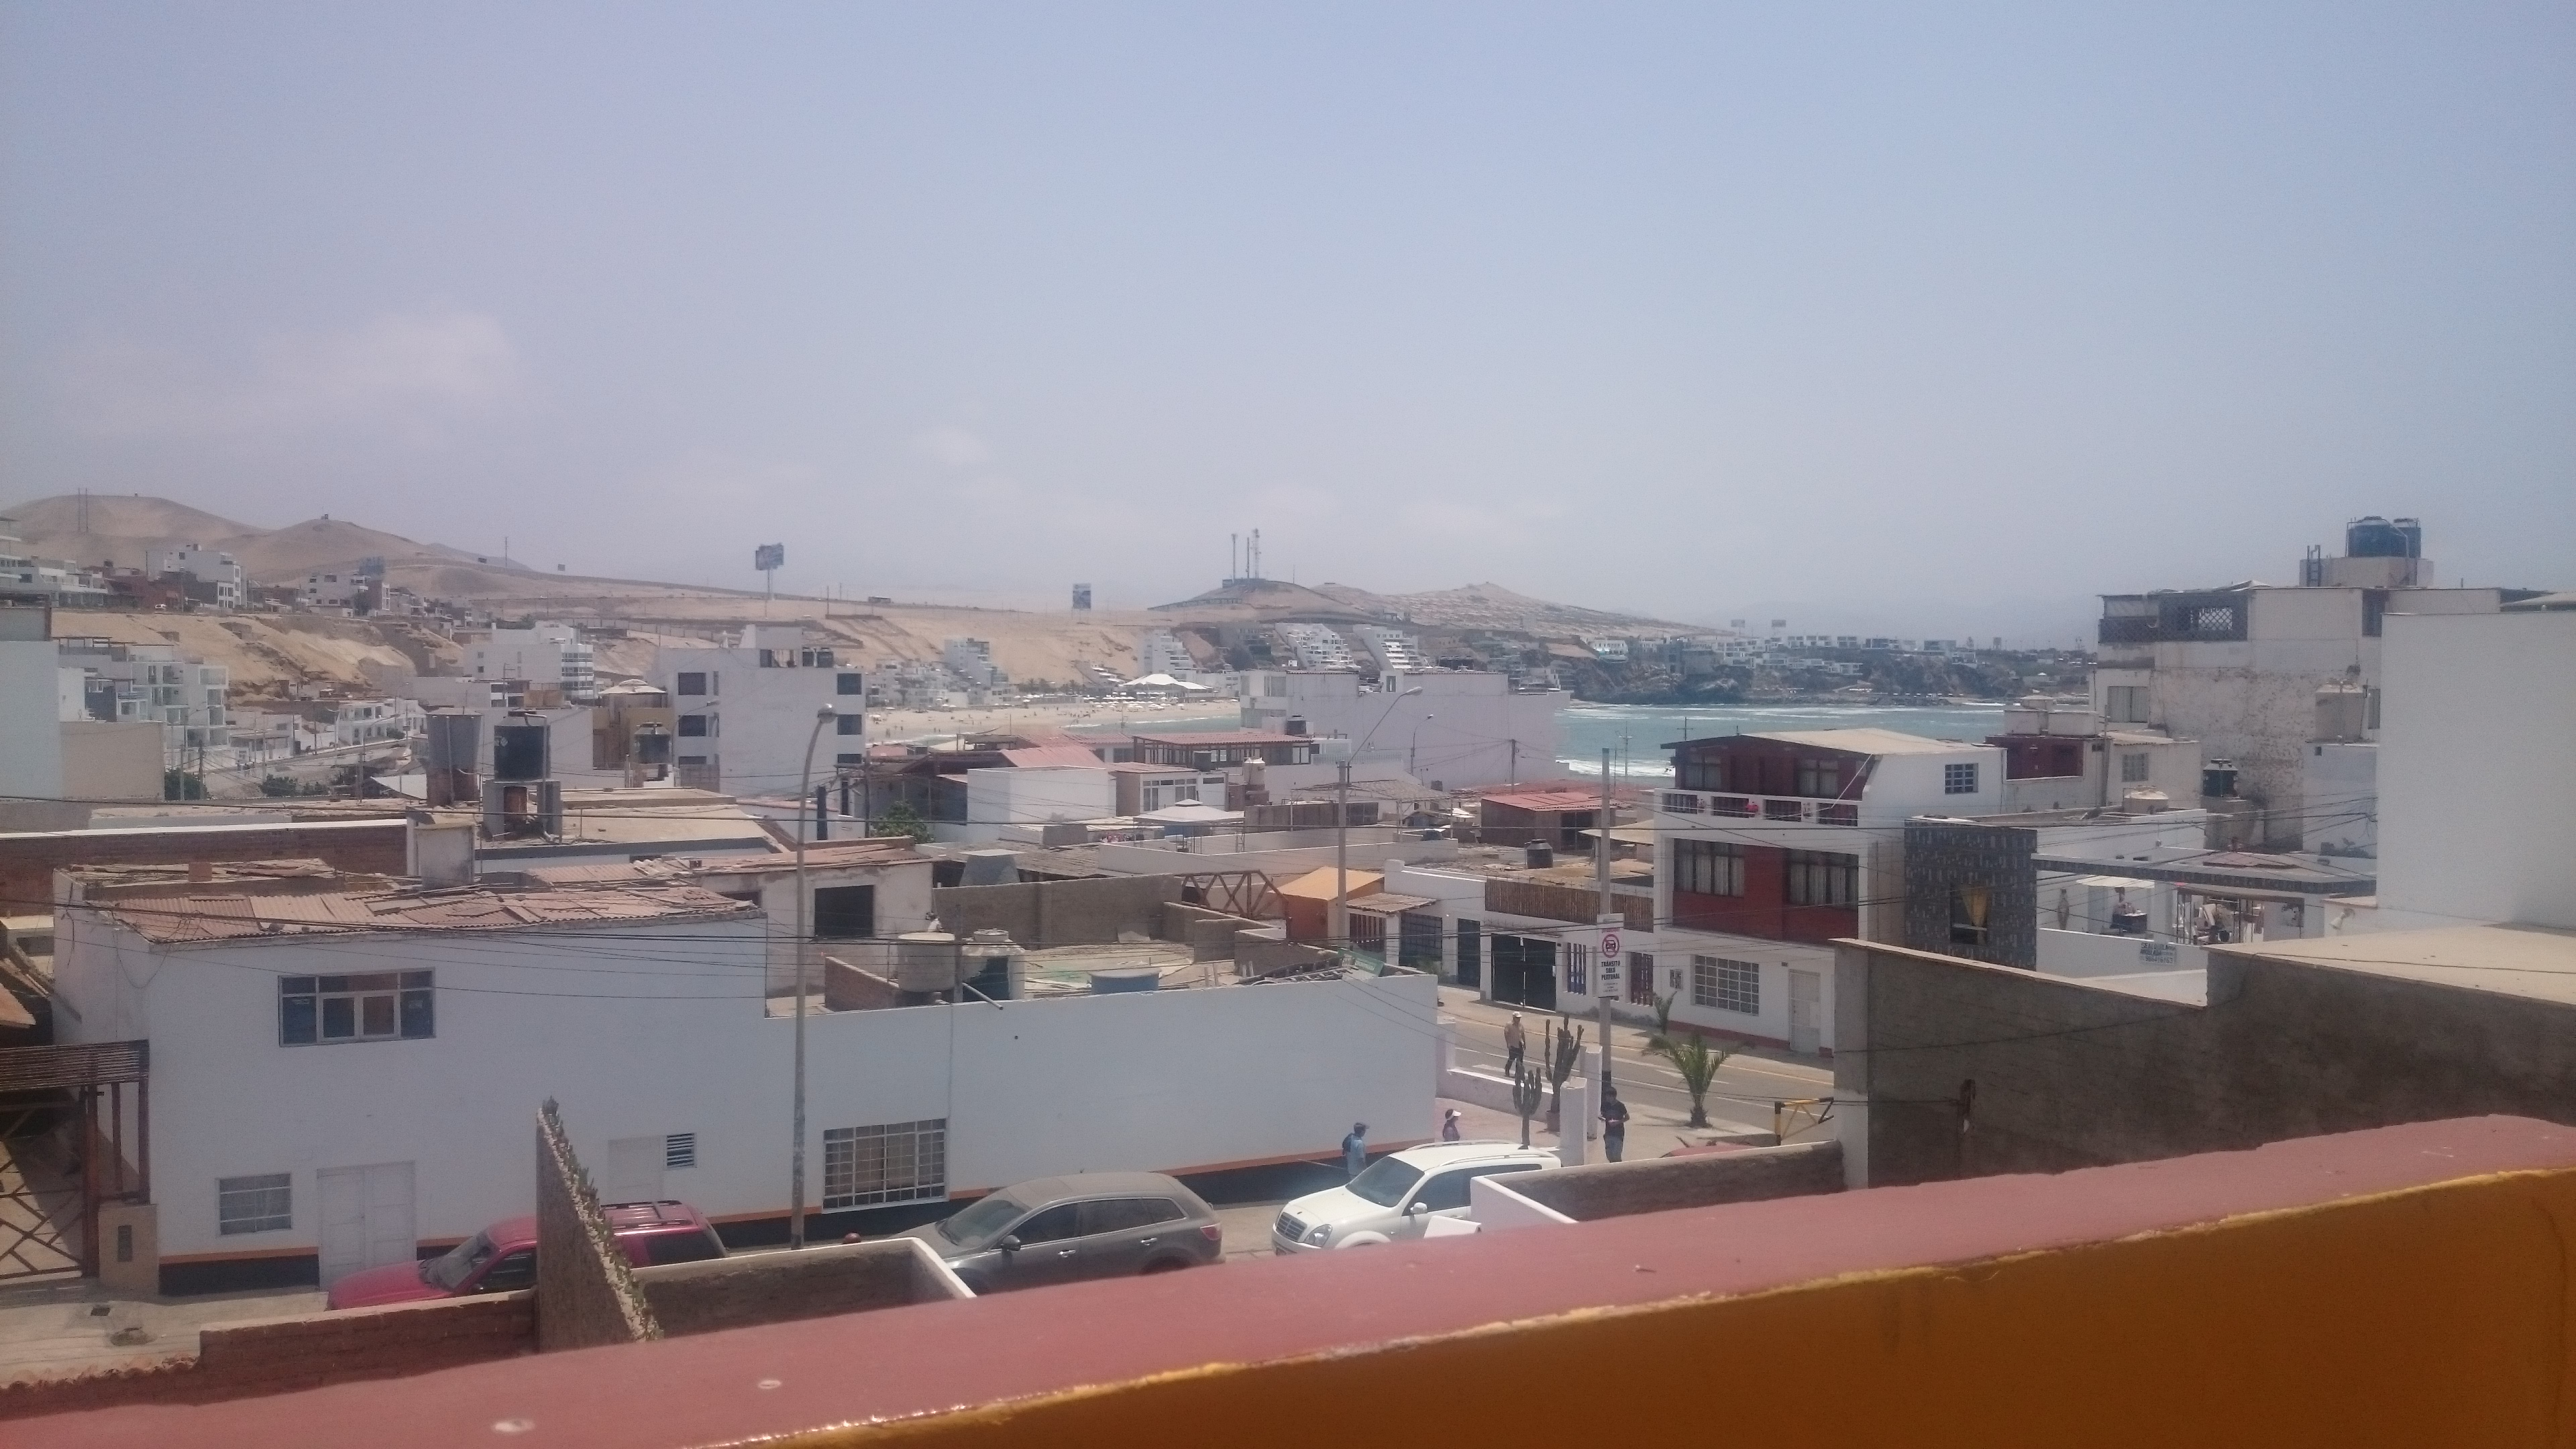
\includegraphics[width=\textwidth]{takeroppskrytt}
	\caption{Tak er oppskrytt}
\label{fig:takeropskrytt}
\end{figure}
En kjapp busstur (les taxi) fra Lima er vi kommet til Punta Hermosa,
en fin surfespot\ldots Og det var det eneste det var. Ellers var det en
spøkelsesby. Marius og jeg var sirka like gode da vi
surfet sammen i Asia (les: jeg var litt bedre), men etter et semester i Brasil hadde han dratt
fra meg (les: han gruste meg). Imidlertid var det langsom break og jeg fikk tatt
mye jeg også. Men en spade er en spade og surfing er padling. Hver dag
bestod av padling,
svelging av interessante mengder saltvann, vasketromling og et glimt
i ekstase som gjorde det verdt å dra ut neste dag. Slik holdt vi på en
uke. I seng 21:00 opp 07:00. Surfing to ganger dagen. Treningsleir.\\



Også i Punta Hermossa var det mange hus uten tak. Vi forhørte oss litt
om dette og fant grunnen. Lima-området er nemlig ørken. Det regner
aldri. Ordentlig tak er derfor en unødvendig utgift. Myndighetene
syntes dette så stygt ut og begynte å gi skattefradrag for folk som
bygget på huset sitt. Her slo Cobra effekten (Google it!
Er gøy lesestoff) til for fullt, for nå var det plutselig gunstig å ikke
ha tak. Man var jo enda i byggefasen!


\begin{figure}[h]
	\begin{center}
	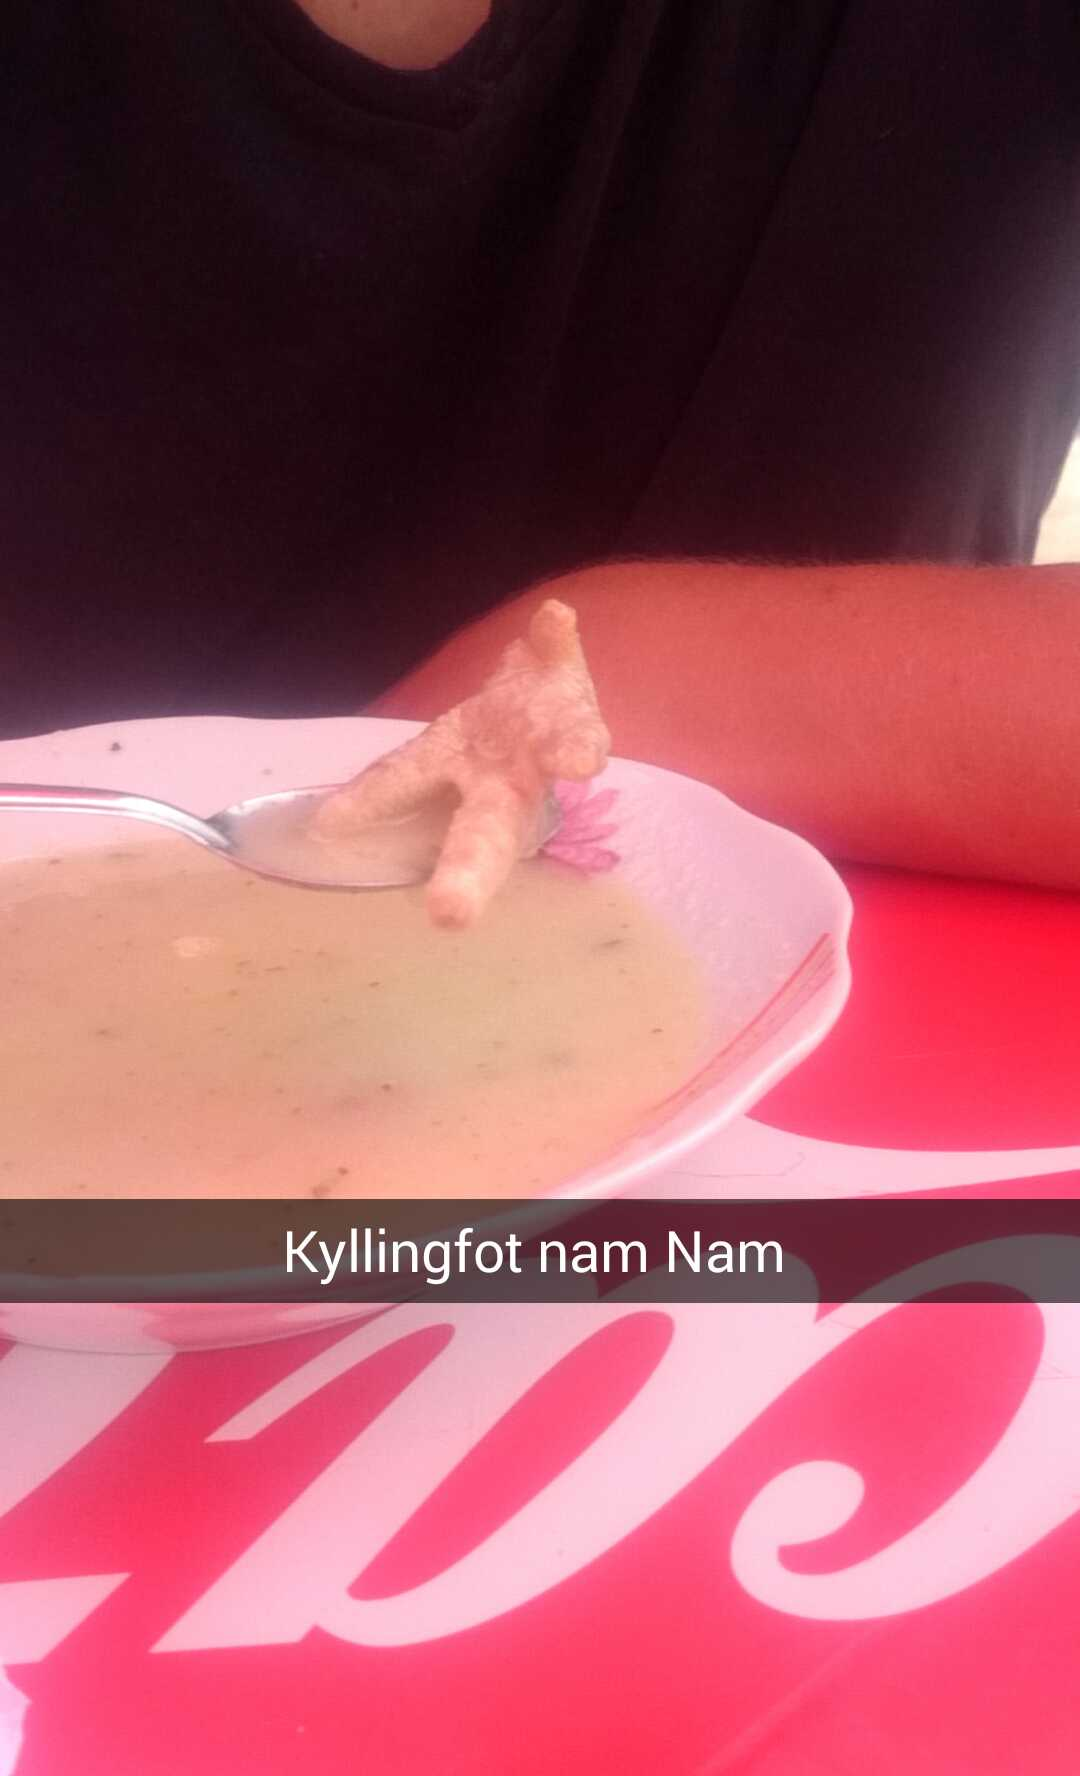
\includegraphics[width=0.48\textwidth]{kyllingfot}
	\caption{}
\end{center}
\end{figure}



Er noen ting som er verd å nevne, men man ikke klarer å klemme en
historie ut av, så jeg ramser dem her.

\begin{itemize}
	\item Den beste jusen er manga maracuja-vi testet
			alle
		\item Kaffen smakte bedre før vi visste den var
			mikrovarmet
		\item Kyllingføtter smaker ikke så ille
\end{itemize}


\subsection*{Treningsleir del 2}

\begin{figure}[!h]
	\centering
	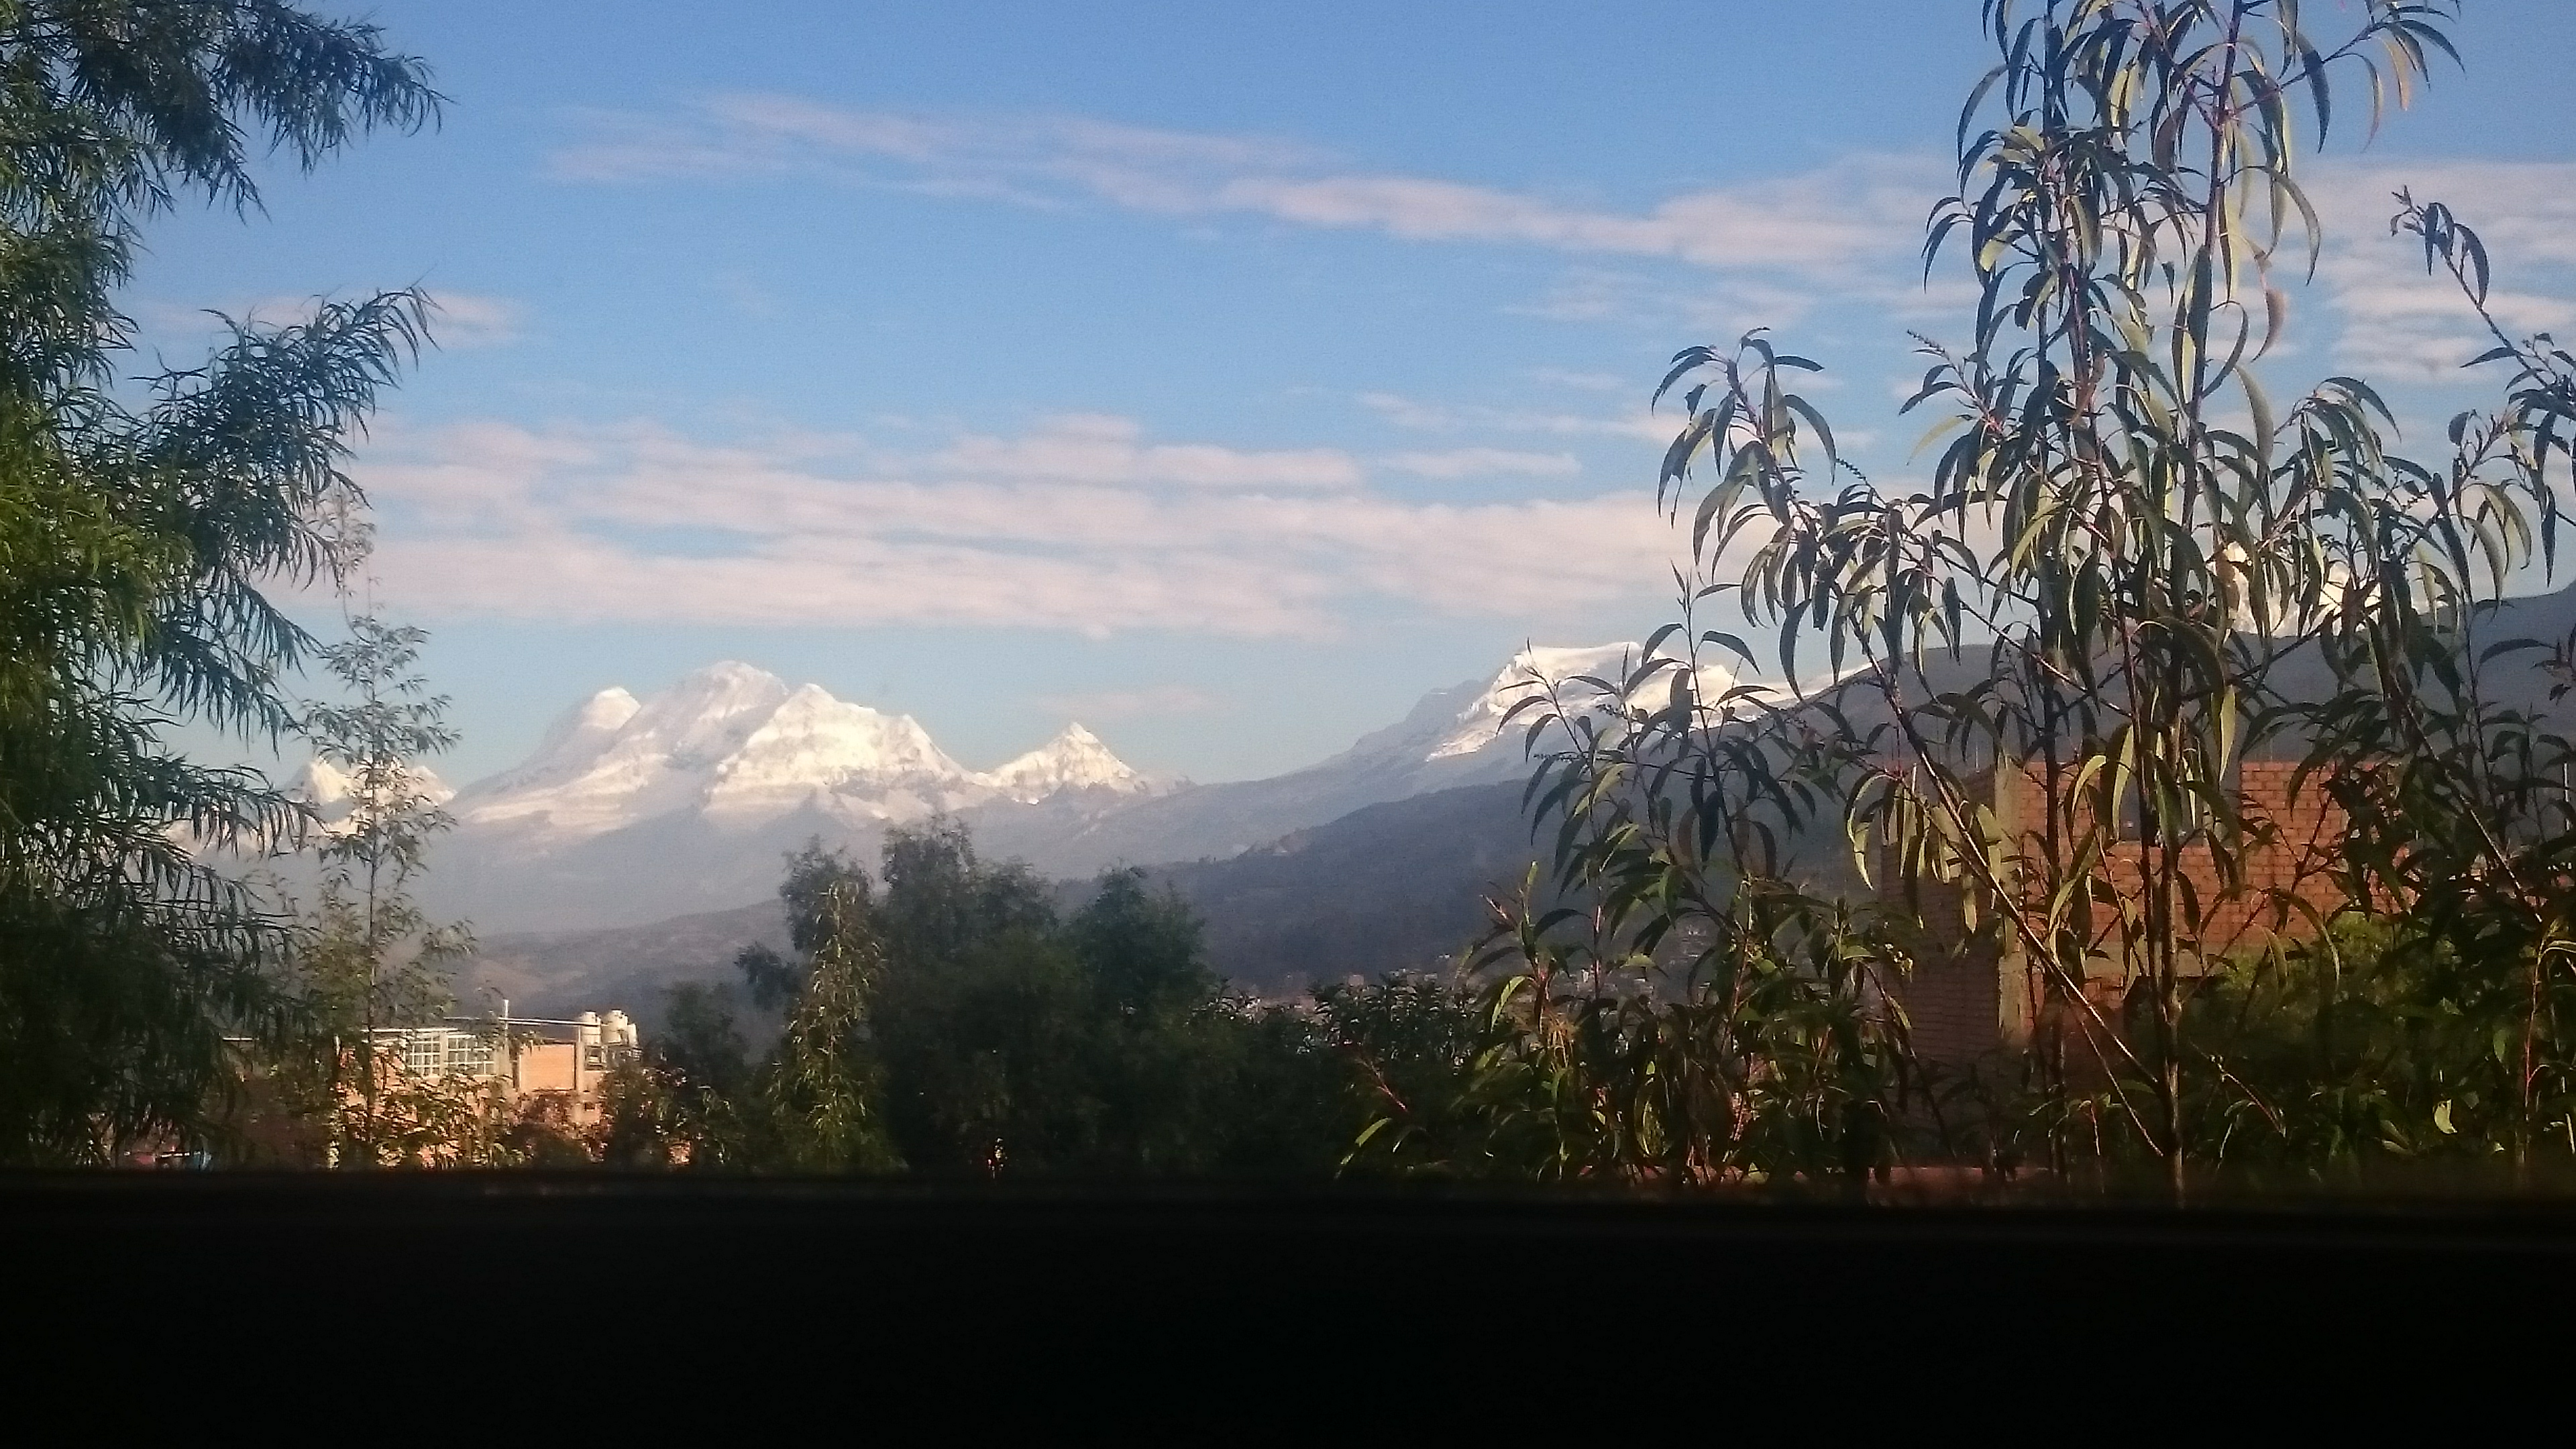
\includegraphics[width=\textwidth]{Hotellromhuaraz}
	\caption{Huaraz fra hotelrommet}	
\label{fig:huaraz}
\end{figure}
Etter en ukes tid har vi fått nok core av padlinga og er klare for
litt høydedoping. Vi bestiller nattbuss og gjør oss klare til å
Andesfjellene. Nei, ikke Machu pichu. Skal opp i den ville
fjellheimen! I Sør-Amerika går ingenting på Engelsk. I allefall ikke
beskjeder til massene på terminal\ldots Den fjerde
gangen vi spurte om oppropet på høytalleranlegget var vår buss fikk vi
en egen plass ved siden av skranken der hun lovte å si ifra når det var vår
tur. \#Jeg-reiser-alene. Bussen var luksus. Setet gikk hele 160 grader!
Vi sluknet som lys. Ble imidlertid vekket av en utrolig frekk kar som
filmet oss i ansiktet. Vi trodde først det måtte være en landsbyidiot
med en sær hobby. Finner senere ut at det er for å vite hvem som var
på bussen om den blir kapret. Good times. 


2800 meter over havet finner du fjellbyen Huaraz. Kan virke som en
landsby med første øyekast. Andre og tredje også. Til tross for dette
bor det flere her enn i Kristiansand. Første dagen tok vi det helt
rolig for å avklimatisere. Vi  fikk også tips om å drikke mye te med coca-blader
ettersom det skal hjelpe mot høydesyke. Vi gaflet innpå. Høydesyke ble
vi. Planen var å gå en fire dagers tur med guide gjennom
Andesfjellene. På det høyeste går man over et pass på ca 5000 meter. Den tredje dagen i
Huaraz var marsjstart. Dag 1 gikk til hvile og  dag to var det
oppvarming på planen. Tingen med
høydesyke er at opp og ned på samme dag sjeldent er et problem. Sove i tynn luft er
derimot en helt annen sak.\\

Andre dagen tok vi derfor turen opp til Laguna Churup i
strålende sol. Dette var den første og beste dagen i
Andesfjellene\ldots  Resten
var mye hating. Men, men er opplevelse det også. 
Vi dro nemlig opp i fjellene i det som lokalbefolkningen kaller for
regnsesongen. Regn forventet vi, men ikke i mengdene som kom! Alle bildene
herfra og ut er mest sannsynlig fra den første dagen vi tok til Laguna
Churup.\\ 



\subsection*{Santa Cruz}

\begin{figure}[!h]
	\centering
	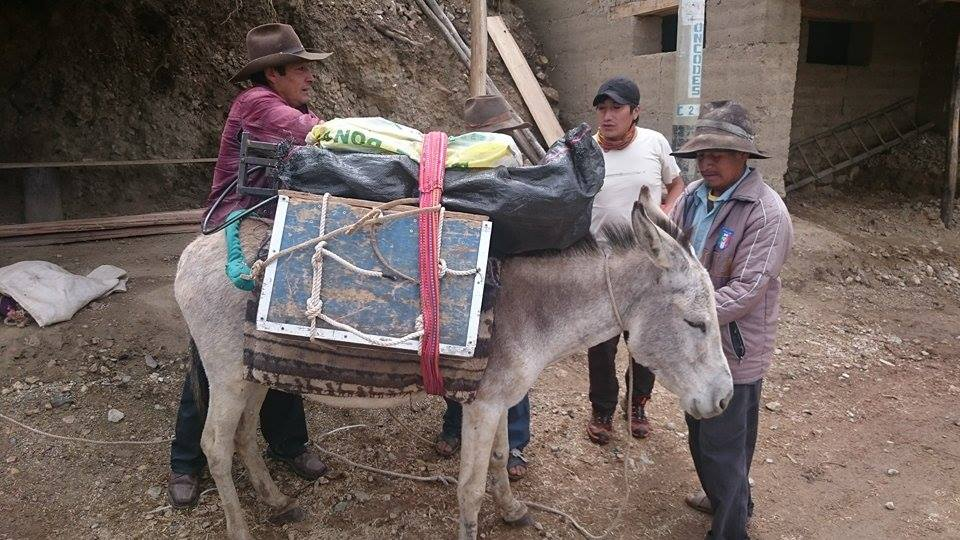
\includegraphics[width=\textwidth]{esel}
	\caption{Pakkeselet}
\label{fig:pakkesel}
\end{figure}

To eseler, en eselritter, en indianer-guide, to jøder og Marius og jeg
starter på Santa Cruz track ved 2700m. Utover 4 dager tar den tar oss opp på 4850 og
ned på andre side av Andesfjellene. Marius og jeg orket ikke drasse på
svære tursko så vi har joggesko. Noe jødene i proft utstyr fant veldig
morsomt. Vi satt dem raskt på plass med å dryle litt sunt hu-og-hei
tempo oppover de første timene. Så begynte det å gå nedover. Med oss.
Veien slynget seg nådeløst oppover. Først fikk jeg gradvis hodepine
mens luften ble tynnere. Så begynte det å regne. Vi slo leir for
dagen og kom oss inn i teltet. Vi fikk en ny virkelighetsoppfatning av
sverden utenfor NTNU da vi startet å
lage mat. Jentene spiste nemlig bare cosher. Som jeg forstod det kan
man ikke spise skalldyr eller blande kjøtt og melk. Kan heller ikke
lage mat i en kjele som har blande kjøtt og melk. Dette er fordi Gud
vil bli veldig sint om man gjør det. Vi prøvde å få den historiske
bakgrunnen til det. Det visste de imidlertid ikke. 
\begin{dialogue}
	\item ``We don't make the rules, we just follow them'
\end{dialogue}
Var svaret vi fikk. Med nød og neppe klarte jeg å
holde inne en Nurnberg kommentar. Var enda 3 dager igjen sammen.\\

\begin{figure}[!h]
	\centering
\noindent\makebox[\textwidth]{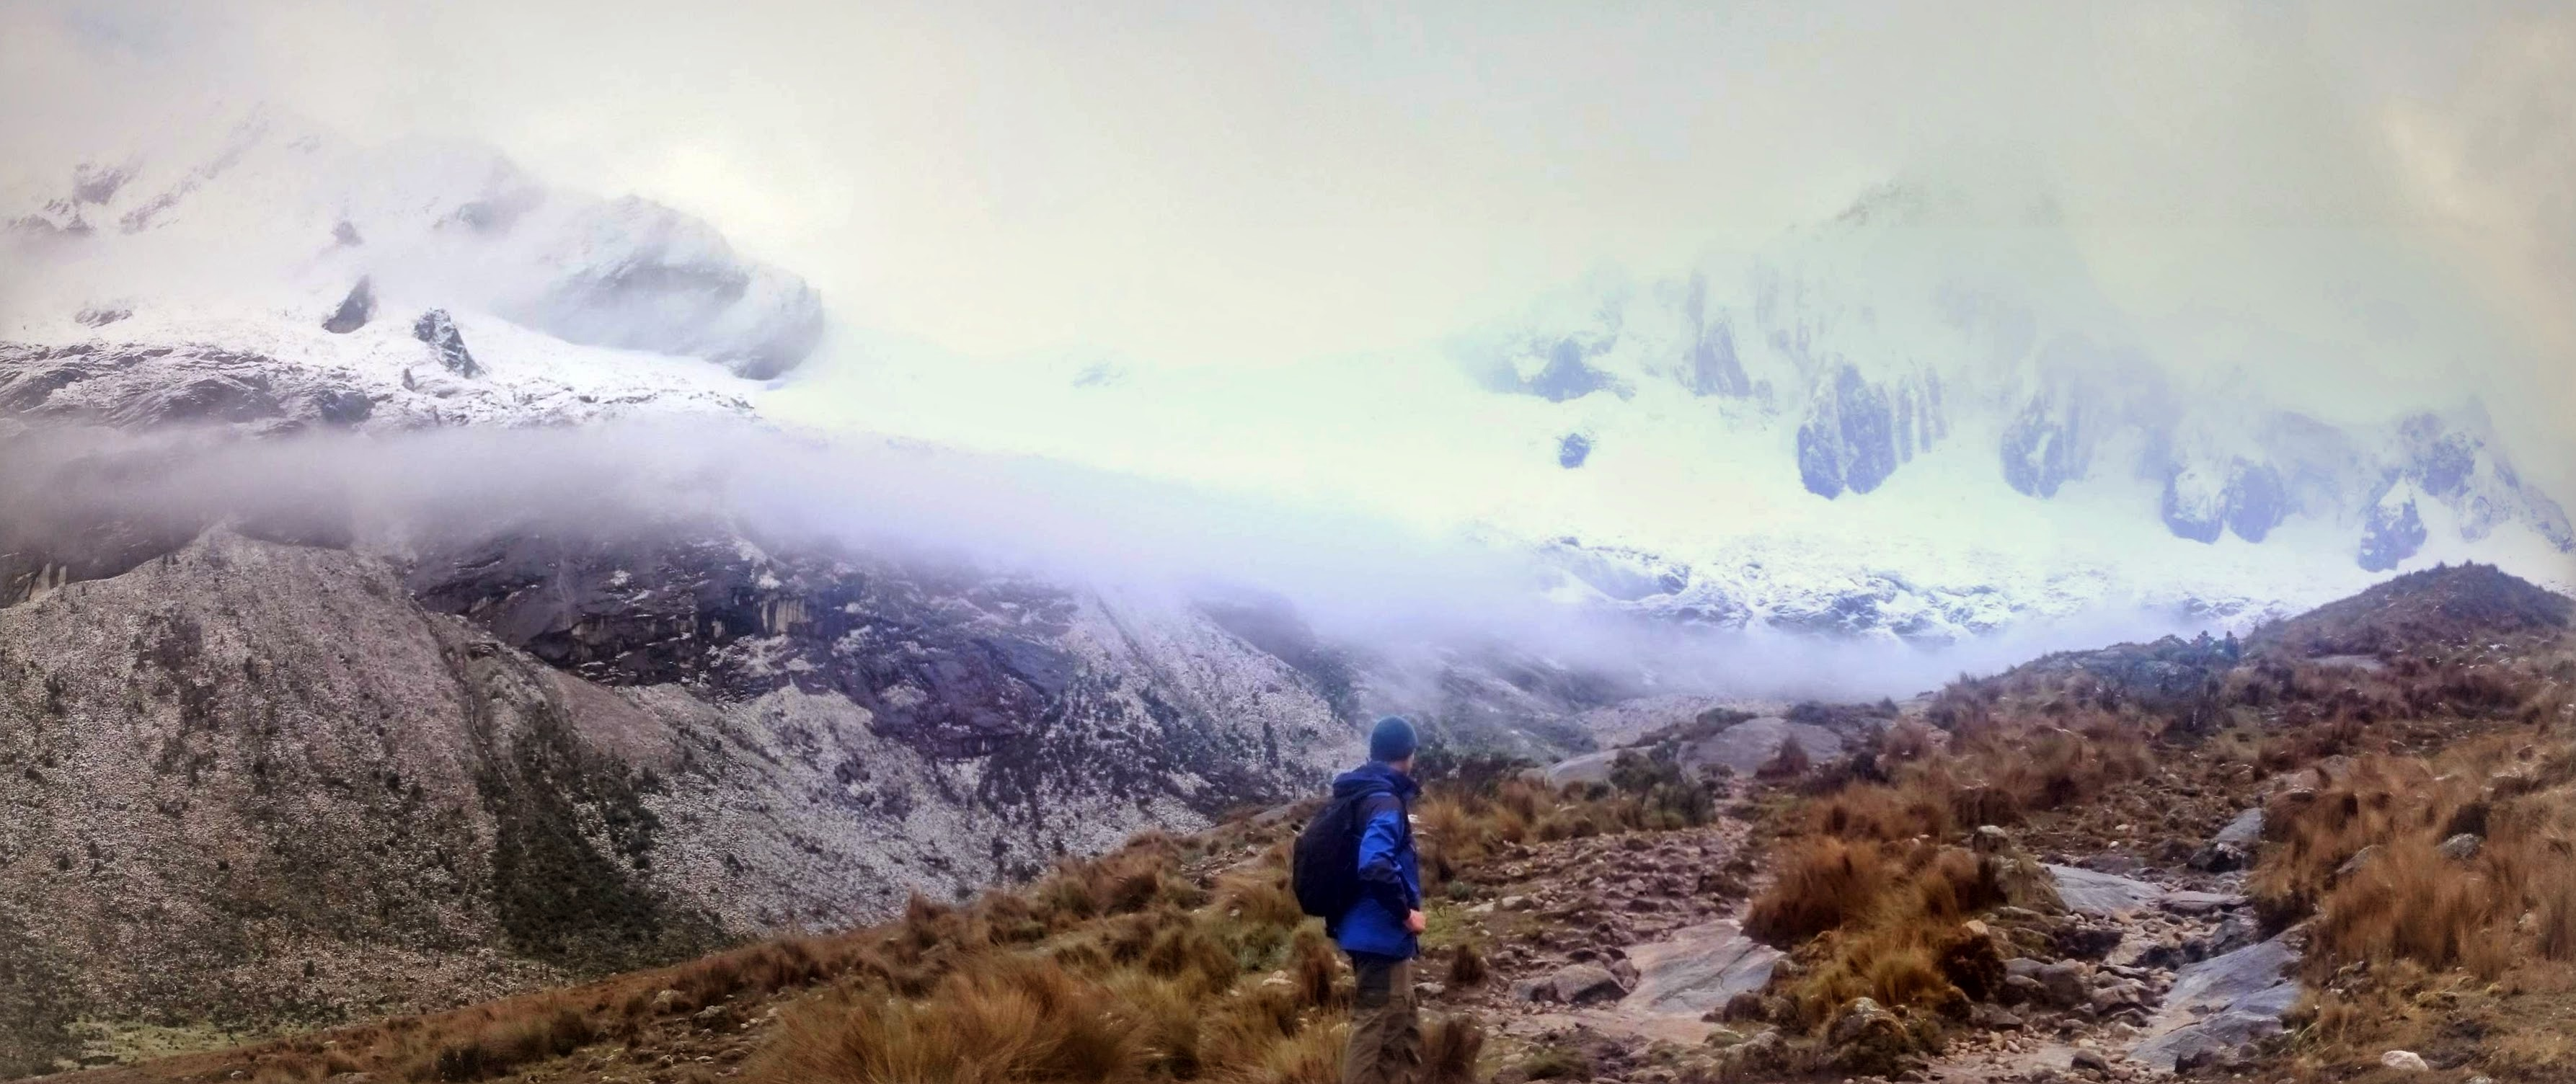
\includegraphics[width=\paperwidth]{Andesfjellenemarius}}%	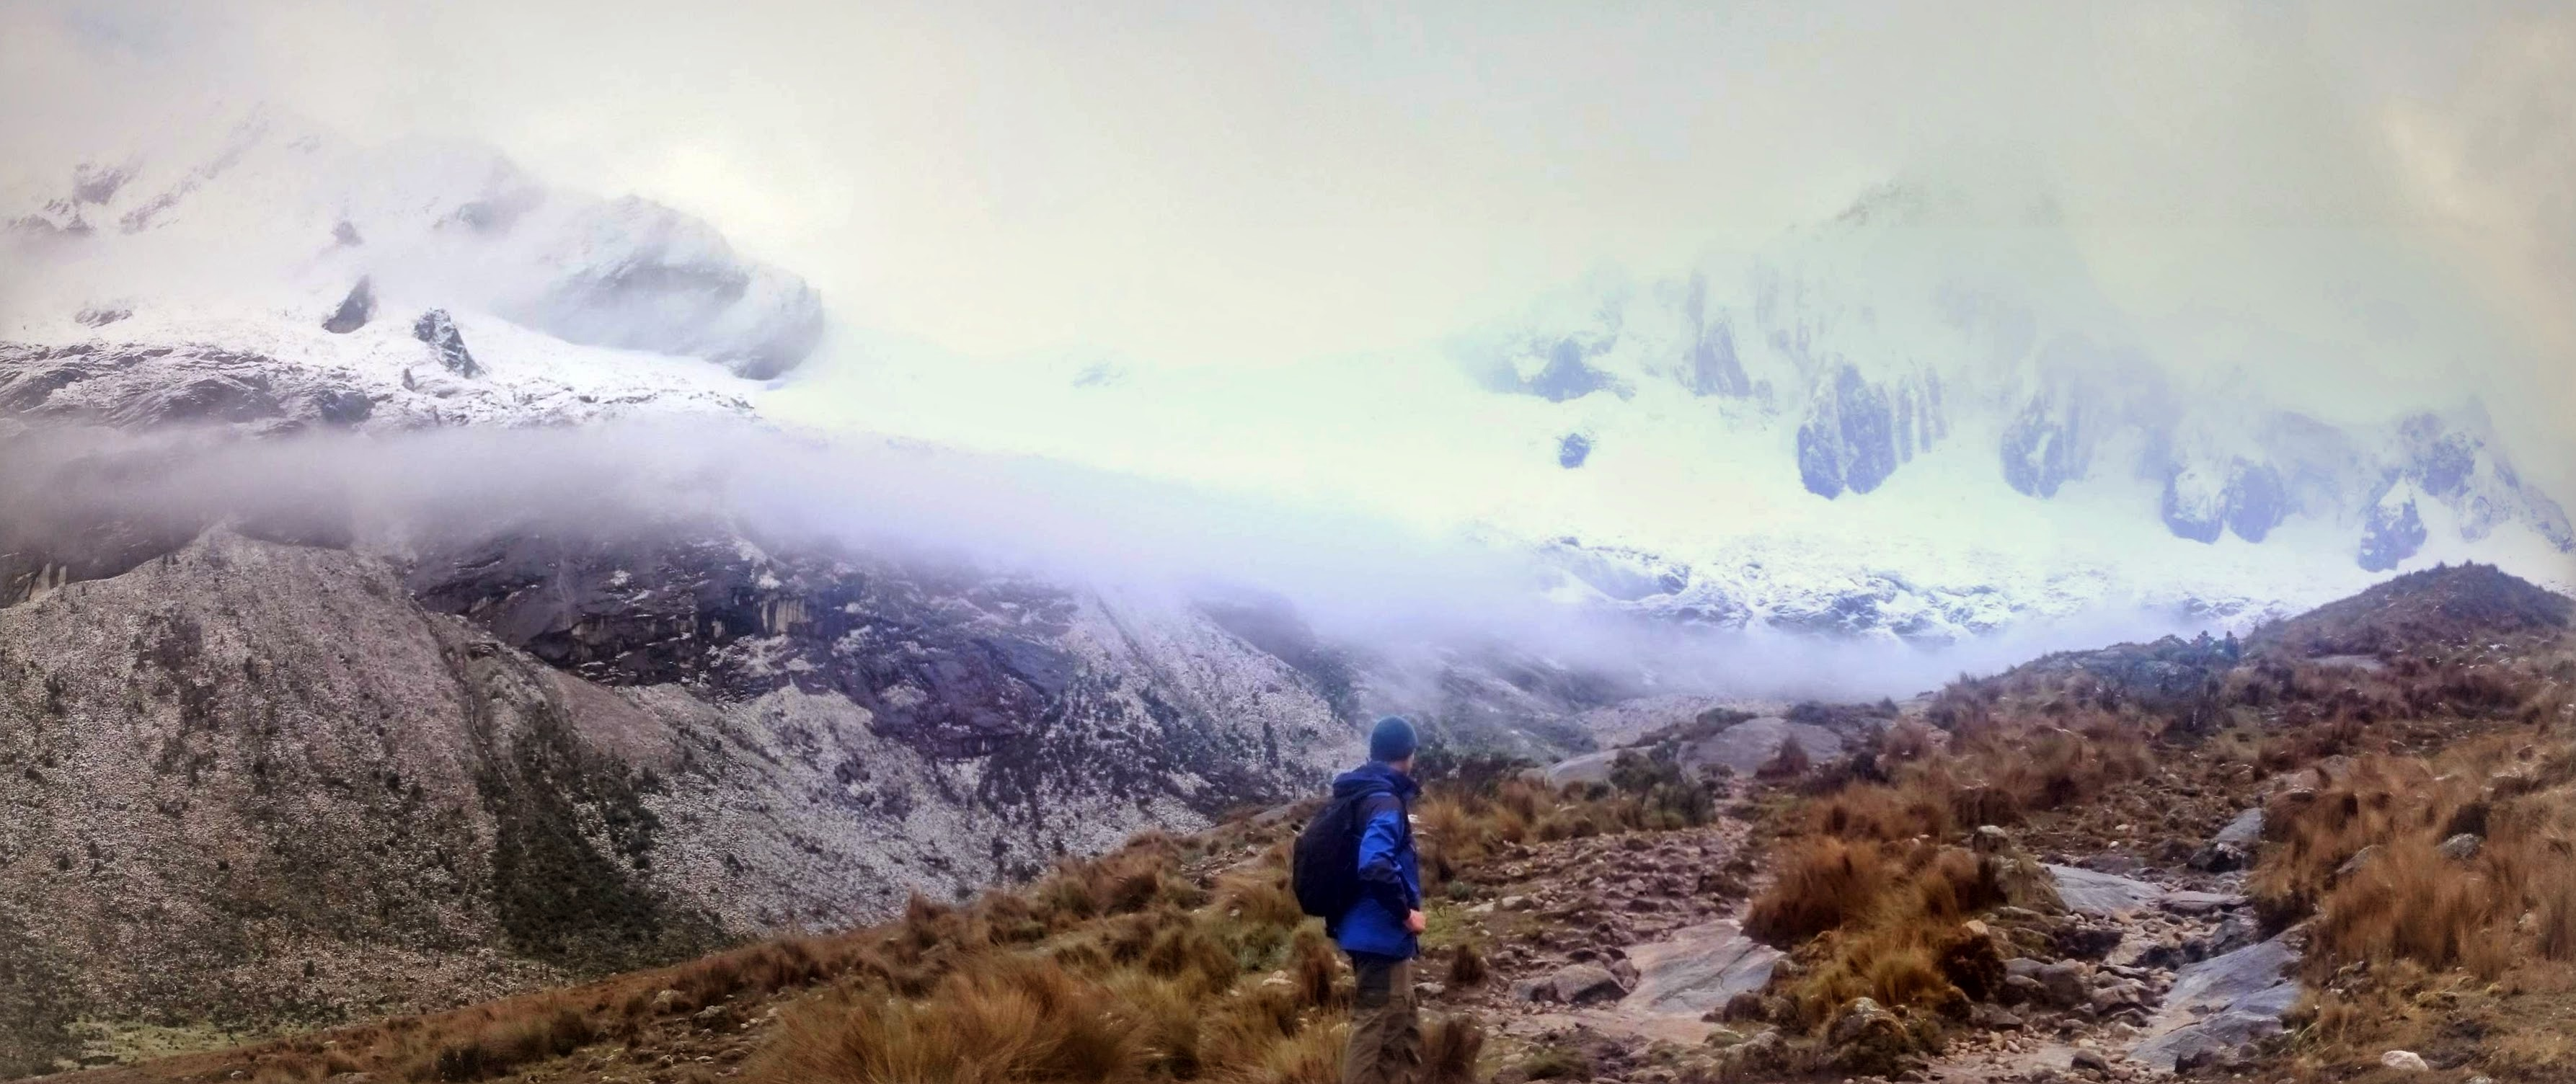
\includegraphics[width=\textwidth]{Andesfjellenemarius}
	\caption{Godvær}
\label{fig:godvaer}
\end{figure}

Som nevnt er Peruanere korte. Det er også teltene deres. Det
ledet til at jeg og spesielt Marius er borti duken med bena når vi
ligger. Nevnte jeg at det regnte? Det har ikke sluttet. Vannet trekker
inn gjennom duken og inn i
soveposen. Etter første natten er soveposene våre gjennomvåte fra
knærne og ned. Fra og med da var det bare sove i fosterstilling. \\

For
hvert steg vi gikk fikk jeg vondere i hodet og Marius fikk dårligere og
dårligere mage. So ordløst trasket vi oppover mens regnet gikk over
til hagl og pisket oss i ansiktet. Joggeskoene våre fikk inn nytt
isvann hver gang vi krysset en bekk med smeltevann. Spikkeren i kista
var at jødene ikke kjente på høydesyken i det hele tatt. Vi gikk
fortere, men de koste seg. Det kan høres ut som jeg er veldig bitter
når jeg skriver dette. Det stemmer ikke. Jeg er veldig glad for at jeg
dro på den turen. Til tross for å være våt, ha hodepine og å sove i
en ball var det enn opplevelse jeg ikke ville vært foruten. Dessuten
hadde jeg den beste makkerene å hate ilag med som tenkes kan. Den
eneste sutring fra Marius var med stor
humoristisk undertone og fikk oss begge til å le!
\begin{figure}[!h]
	\centering
	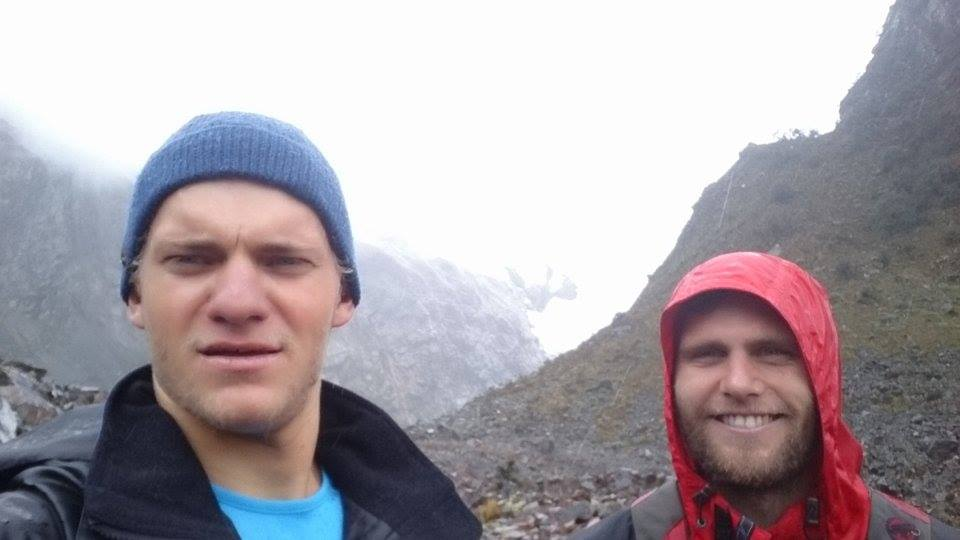
\includegraphics[width=\textwidth]{akselogmariusiregn2}
	\caption{Humøret holdes opp!}
\label{fig:turiregnet}
\end{figure}
\subsubsection{There and back again}
Noen ganger i livet er du nødt til å legge skjebnen i andres hender.
Bilturen ned Andesfjellene var et slikt øyeblikk. Bilen var en
skranglete van med litt for høyt tyngdepunkt. Veien slynget seg
nedover berget med krappe svinger uten autovern. Hver sving hadde et
drop på alt fra klatreullyke-død til flystyrt-død. I disse svingene
kjørte peruanerne over 50 og man følte at vekten på hele
bilen la seg over på hjulene nærmest stupet. Heldigvis var det tåkete,
så man så ikke helt hvor bratt det var. Men igjen, det gjorde ikke
sjåføren heller \ldots Etter en halvtime med hjertebank er den eneste
måten å komme seg gjennom på å si til seg selv: ``dør jeg så dør jeg,
i det minste er det ikke 5 mil fra der jeg ble født!'' Så i den 4
timers lange turen kaldsvettet jeg og hoppet på humpelene så jeg slo
hodet i taket. Hvordan tok Marius det? Han sov hele veien. Våknet
såvidt da han dunket hodet så hardt i kneet mitt at han fikk et
blåmerke. 

\begin{figure}[!h]
	\centering
	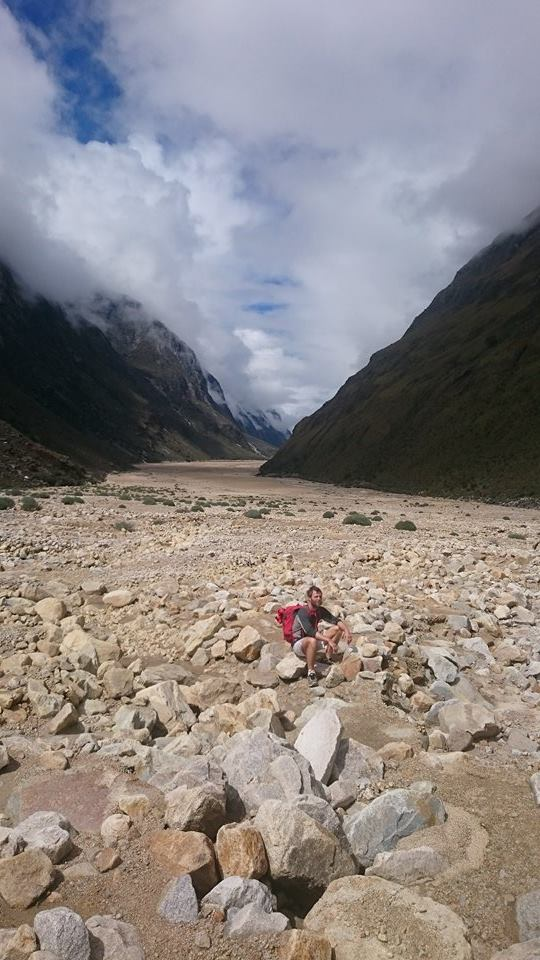
\includegraphics[width=0.7\textwidth]{akselidalen}
	\caption{På vei opp}
\label{fig:akselidalen}
\end{figure}

\clearpage
\section*{Colombia}

\begin{figure}[!h]
	\centering
\noindent\makebox[\textwidth]{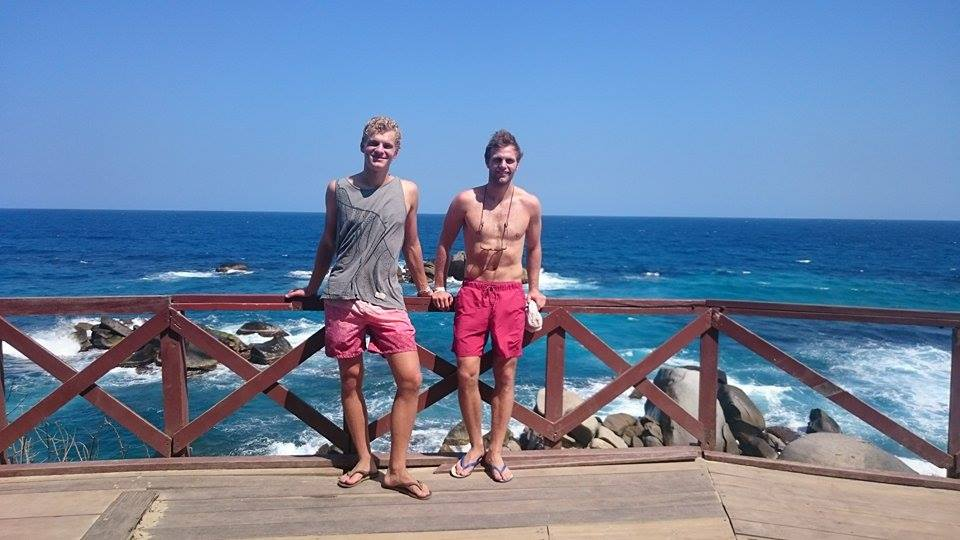
\includegraphics[width=\paperwidth]{stjernerinationalpark}}
	\caption{Stjerner i nasjonalparken}
\label{fig:colombia}
\end{figure}

\subsection*{Medillin}
I løpet av min reise i Sør-Amerika var det ingen by som ble like mye
anbefalt som Medillin. Noe som er ironisk ettersom det for bare 20 år
siden var regnet som verdens farligste by. Da under jernhånden til
narkotikabaronen Pablo Escobar. Narkotikaproduksjonen er imidlertid
bare en plett i Medillins kompliserte, triste og utrolig interessante
historie.  \\

Da spanjolene kom til Sør-Amerika var de fleste på jakt etter gull.
Medillin er utrolig kronglete å komme seg til. Selv idag er egentlig
den eneste oppegående måten å fly. Om ikke må du
pine deg gjennom en 18 timers busstur gjennom svingete veier og fuktig
jungel. Spanjolene dro heller mer tilgjengelige steder for å grave
gull. Det var imidlertid to folkeslag som ikke var så interessert i
gull. Frihet var det de var ute etter. Begge folkeslagene ble
forfulgt i Spania. Det ene var en liten gruppe mennesker som holdt
til i foten av pyreneene ikke så langt fra grensen til Andorra. Navnet deres har dessverre gått i
glemmeboken. Det andre forfulgte folkeslaget var, tradisjonen tro,
jødene. Et pent sjakktrekk er det jo da å slå seg ned et sted det er
megastress å komme seg
til.\\

Skjebnen hadde det slik at det var masse gull i Medillin. Noe
etterkommerne til disse to folkeslagenene (nå kalt paisas) ble veldig
rike på. Medillin ble en stor industriby og fikk bl.a den første
jernbanen i Colombia. Historien til Medillin etter dette er utrolig
komplisert. Dette er det jeg husker fra den allerede forenklede
forklaringen til guiden:

\begin{itemize}
	\item Regjerinen var blå og folket rødt -- væpnet opprør
	\item Regjeringen nå av rød, indre splid -- væpnet opprør
	\item Regjereingen midt i mellom. Væpnet kamp mellom blå og
		rød side av folket. Regjeringen fornøyd med at de får
		være i fred
	\item Regjeringen går inn for å ødelegge narkotikaplantasjer
	\item Rød og blå folkehær leid inn av narkotikakartell for å
		passe på plantasjene
	\item Paramilitære gjør glidende overgang fra å representere folket
		til å bli
		leiesoldater for narkotikakartellet
	\item At folkehærene drar til jungelen for å passe på
		plantasjer gir Regjeringen mer kontroll over byen. Da
		spesielt som følge av døden til Pablo Escobar.
	\item Landsbyene er enda kontrollert av lokal gerilja leid inn
		av narkokartellet

	
\end{itemize}

Alt, noe eller ingenting av det jeg sa over stemmer. Det som du
trenger å ta med deg er at det er har vært mye slåssing og like mange
sider. Det jeg vet helt sikkert er at det er no-go å krysse grensen ut
av Colombia med bil. Det er å be
om å bli kidnappet. Blå øyne vil ikke gå til din fordel her heller!\\

Medillin har fått mye internasjonal ros for hvordan de har pusset opp byen.
Etter at narkotikakartellet har hatt så mye makt så lenge var mange av
byens strøk mildt sagt shady. Det er de enda. Mens jeg var der ble en
turist knivstukket siden han gikk seg vill og havnet i en
gjenkontrollert gate. De var imidlertid veldig barmhjertige og
knivstakk ham bare i skuldra. En vennlig advarsel rett og slett.
Uansett, oppussing. Istedenfor å bygge opp et fint strøk er taktikken
å sette noe fint i et veldig tvilsom strøk. For eksempel
bygget de et offentlig bibliotek i det som var det verste
dealerstrøket i byen. Følgende kom mange fornuftige folk til denne
delen av byen for å studere. Plutselig var ikke denne delen av byen så
farlig likevel. Kanskje det ikke gikk fullt så silkeglatt, men det er
konseptet i det minste!
\subsubsection{Kirkens paradoks}

\begin{dialogue}
	\item ``I would have asked God for a bike,
	\item but i know he doesn't work that way
	\item so i stole one and asked for forgivnes'
\end{dialogue}\\ -Hvilken som helst Colombianer

\begin{figure}[!h]
	\centering
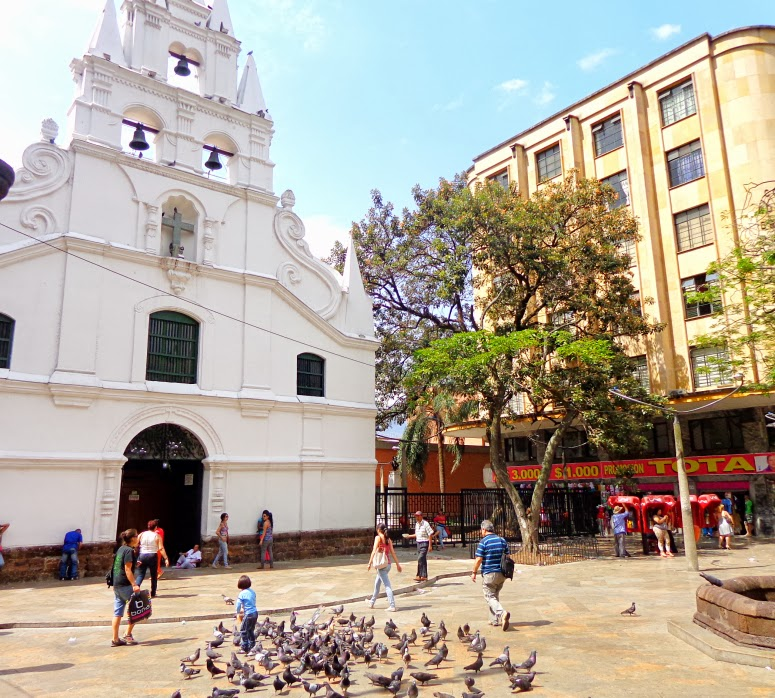
\includegraphics[width=\textwidth]{workinghard}
	\caption{Damene i telefonkioskene skal ikke ta en telefon}
\label{fig:prosti}
\end{figure}
Colombianere har et veldig praktisk synd på kristendommen. Ikke
praktisk som i fornuftig eller sekulært. Praktisk som i at du kan gjøre
hva du ville så lenge du ber om tilgivelse. Selv den mest blodige
attentatmann ser på seg selv som en god kristen mann- han har jo
alltid skriftet etterpå. Som følge av dette skjer det alltid artige
ting utenfor kirker. Om man først skal synde er det jo greit å kunne
løpe rett inn i kirka etterpå! Dette gjelder alt fra prostituerte til
salg av  piratkopierte filmer. En kjapp en bak kirkehjørne og
rett til skrifteboksen. Alt før lunsj! Og folk sier Sør-Amerikanere er
ineffektive. Er også ganske inspirert å selge Disney- og pornofilmer
side om side.

\subsubsection{Uteliv}

Marius og jeg måtte ut å ta noen drinker i Medillin. Kvinnene her her svært

behagelige på øyet. Når du kommer inn på et utested er det første som skjer
at du blir tilbud litt aguaridente - en loka brennevin. Helt ok. Det
neste som skjer er at jente skal danse med deg. Rettelse: lære deg å
danse. Noe som var gøy den første gangen. Tingen er at de blir litt
frustrert når progresjon til de grader uteblir. I tillegg er det
å danse sensuell pardans utrolig kjedelig om ikke jenta er veldig
veldig pen. Vi tok det heldigvis vi igjen i Panama da vi tok over
dansegulvet med litt god norsk hopping og spretting!

\subsubsection{Local haircut}

Håret vårt hadde blitt ganske langt og ustyrlig så fant ut  at det
kunne være artig å ``skrelle neba'' i en lokal bule. I salongen var
det tre personer. En skallet, en med rottehale og caps og en søt dame.
Marius gitt først inn og endte opp med mr. Rottehale og jeg fikk den søte
dama. Score!Sistemann hev på partymusikk og danset rundt i lokalet. Med
iherdig innsats fikk jeg forklart at jeg ikke vil bruke maskin. Heller
ikke på sidene! Det siste var helt nytt for henne. Siden skal skinnes
i Sør-Amerika. Så var det igang med saksa. I Norge er det vanlig at
frisøren går rundt deg mens hun klipper. Oftest sitter de på en stol
som kan rulles rundt. Her var det omvendt. Jeg satt på en kontorstoll
som kunne snurre 360 grader. Så istedenfor å gå på andre siden spant
hun meg rundt og rundt. Litt svimmel ble jeg, men det hører med.
Hører kanskje ikke med at frisøren klipper seg i fingeren og blør
utover øret ditt. Men, men sånn er bare å ta på strak arm

\subsection*{Latin-Russian og Tayrona National park}

Etter en rask flytur lander vi i Cartagena. Det er i Nord-øst delen
av Colombia og grenser til det Karibiske hav. Marius var lysten på å
dra hit for å møte noen kamerater. Jeg ville snorkle.. I mitt hode var hele det Karibiske hav et snorkleparadis. I
Cartagena var det sand og grums. Usikkert om Marius visste dette og
bare jattet med for å få viljen sin. En suksess ble det uansett! Vi møtte tre NTNU-studenter derav en
hadde bursdag. Dette måtte feires! KGB-bar neste! KGB-bar er som
navnet tilsier dedikert til KGB. Da med komplette rødt interiør,
sigd og hammer i hytt og gevær og viktige historiske bilder fra
kommunistiske Russland. Gjerne med vår gode venn Vladimir åpenbart
photoshopped inn. Det er garantert en historie bak KGB-bar, men den er
klassifisert. Så du får bare nøye deg med å nyte verdens sterkeste
white-russian mens du ser på langer manequiner i full uniform,
pilotbriller og polarluer. 


\begin{figure}[!h]
	\centering
	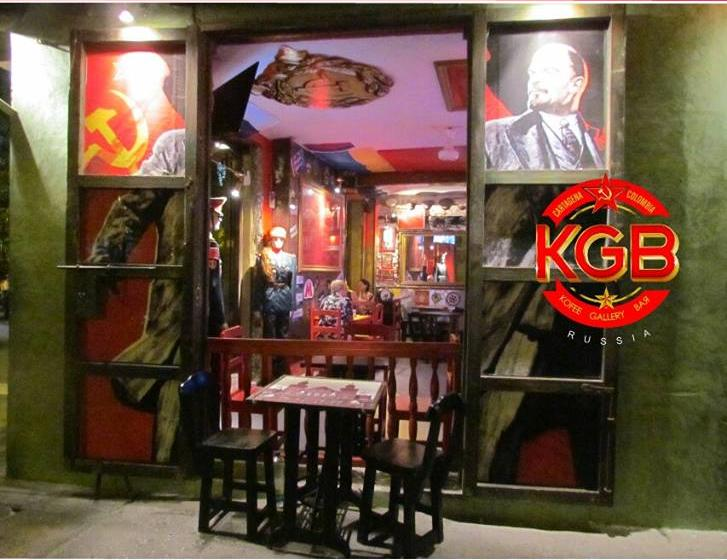
\includegraphics[width=\textwidth]{kgbbar}
	\caption{KGB-bar}
	\label{fig:kgbbar}
\end{figure}\\
\clearpage

Tayrona nasjonalpark var neste destinasjon. For oss. Bagasjen lot vi
ligge igjen på et tvilsomt hostel i Cartagena. Dette ga meg mer angst
enn jeg liker å innrømme. De norske damene som havnet i boliviansk
fengsel var kanskje litt
mer naive, men men hadde angst vært rasjonelt ville ikke jeg
hatt sommerjobb! La oss bare si jeg sjekket bagasjen
grundig da jeg fikk den tilbake. Nevrotisme til side -- vi
skulle vandre i paradis. Tayrona Nationalpark består tett jungel som
klatrer over lave fjell før den brått stopper i hvite strender og det
azure-blå Karibiske hav. Her var det tre ting vi skulle gjøre:

\begin{itemize}
	\item Sove i hengekøye
	\item Bade i azurblått vann
	\item Chille max
\end{itemize}

Som sagt så gjort.

\begin{wrapfigure}{L}{0.45\textwidth}
	\begin{center}
		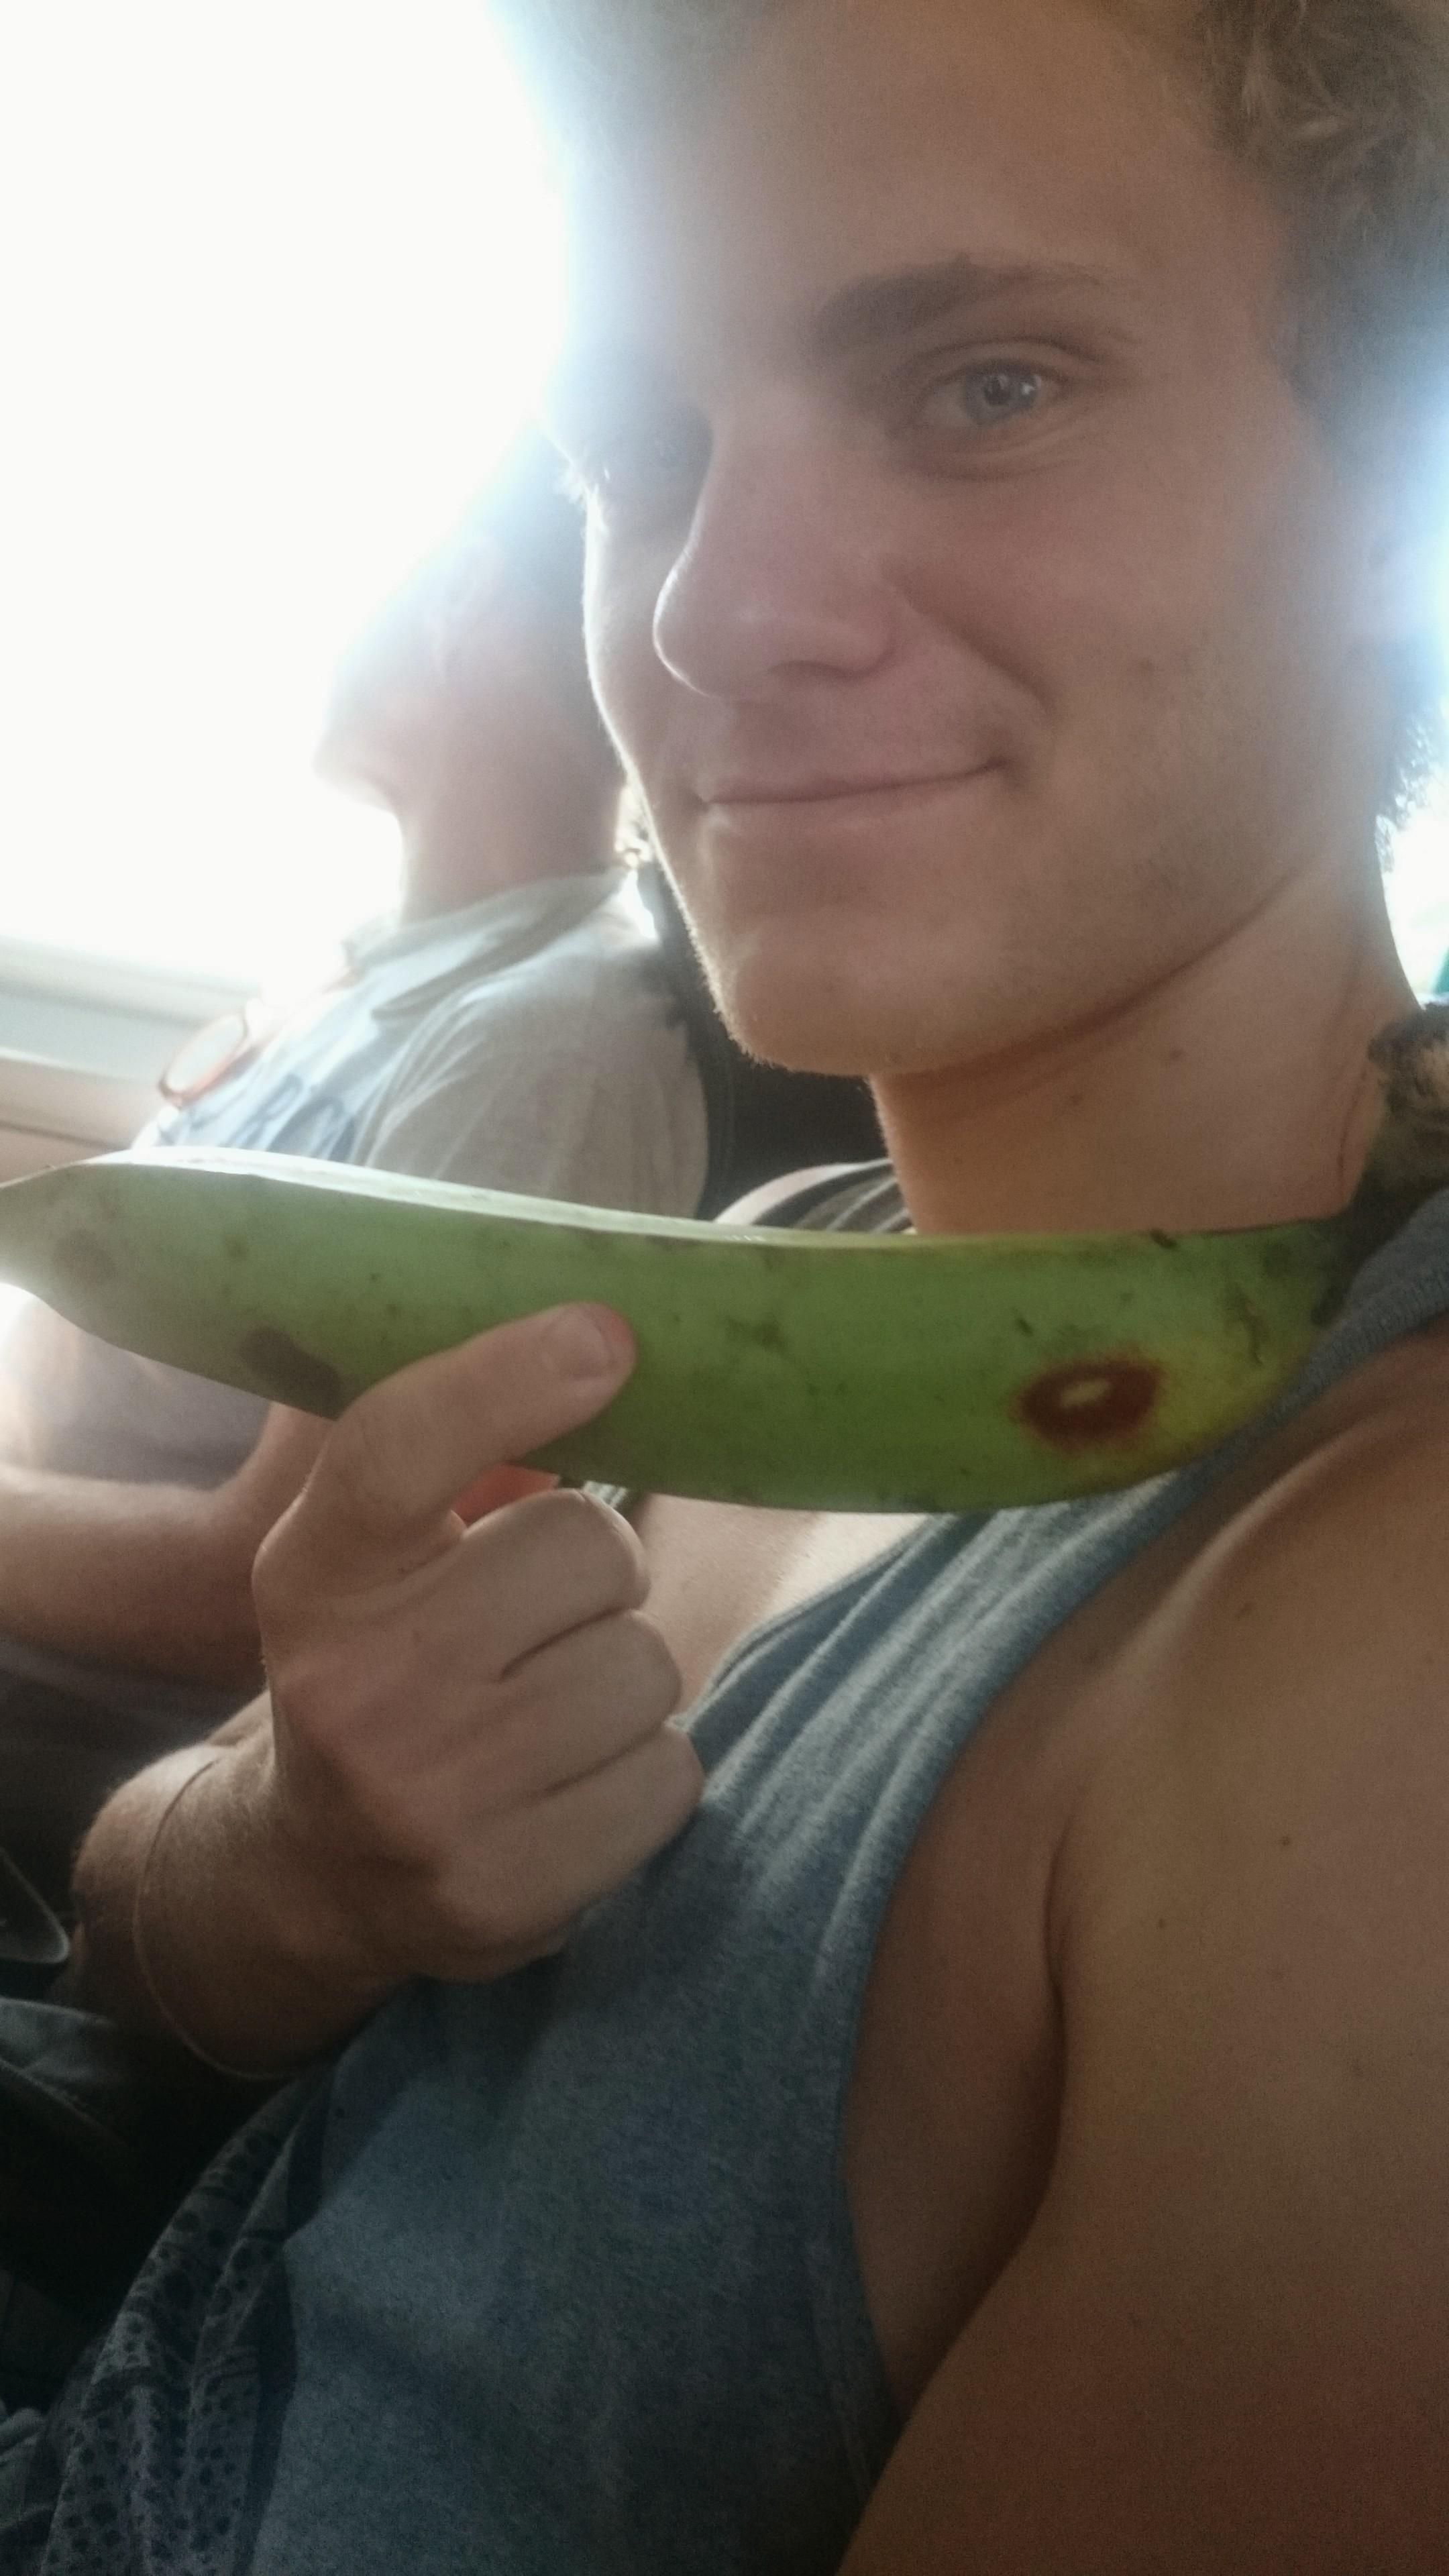
\includegraphics[width=0.30\textwidth]{Kjopmatmarius}
	\end{center}
	\caption*{Forste og siste gang Marius får matansvar
	\#fargeblind}
\end{wrapfigure}
På bussturen opp tok Marius på seg ansvaret å kjøpe
inn litt frukt til turen. Det var siste gang han fikk den oppgaven.
Han sverger enda på at de alle så sånn ut, men han vinner ikke
akkurat  Buskerud-mesterskapet i tyttebærplukking.\\

I løpet av turen har Marius og jeg et pågående sjakkmesterskap. Vi er
pinlige jevngode. Problemet er at ingen liker å ligge å under.
For å holde reisefreden var vi derfor nødt til å spille nok kamper til
at det er uavgjort i seiere triptotal. Dette endte med at vi ble
sittende å spille fire timer straight i en park i Lima. Etter det var
det litt tiltak å ta opp sjakkspillet igjen. Heldigvis hadde Marius
ett ess i ermet. I en bungalow ved det Karibiske hav ble jeg
introdusert for omvendt kasino.


\subsubsection{Hvordan spille omvendt kasino}
Omvendt Kasino blir mye det samme kasino, bare gøyere! Istedenfor
å samle poeng selv skal du prøve å prakke på motparten så mange som
mulig. Alle som har en rival vet at det er langt gøyere å ødelegge for
motparten enn å gjøre det bra selv! Er et eget ord for det på Norsk.
Skadefryd. Passe brutalt. Finnes ikke på Engelsk. Finnes på tysk, men
det kan ikke komme som en bombe på noen. Reglene er som følger:

\begin{itemize}
	\item Den med færrest poeng vinner
	\item Flest kort, ess  og spar2  gir 1 poeng
	\item Flest spar, ruter10 og tabbe(svipp) gir 2 poeng
	\item Man kan ikke legge ut et kort som kan ta noe fra bordet
	\item Man må ta inn en tabbe om motparten melder det
\end{itemize}

Alt her burde være klart bortsett fra den siste regelen. En tabbe er
som en omvendt svipp. En svipp du helst ikke vil ha. Imidlertid hvis
det er noe på bordet som er mulig å ta inn med ett kort kan motparten
melde:
\begin{dialogue}
	\item ``Tabbe (kort)''
\end{dialogue}
Om man da sitter med dette kortet blir man nødt til å ta det inn alle
kortene på bordet og får i tillegg en tabbe som gir to poeng. 

\begin{figure}
\centering
\begin{minipage}{.3\textwidth}
  \centering
  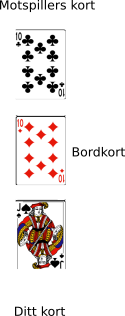
\includegraphics[height=1.5in]{tabbenkel}
  \captionof*{figure}{Om det er motstanderens tur\\  vil du hare si tabbe 10}
  \label{fig:test1}
\end{minipage}%
\begin{minipage}{.6\textwidth}
  \centering
  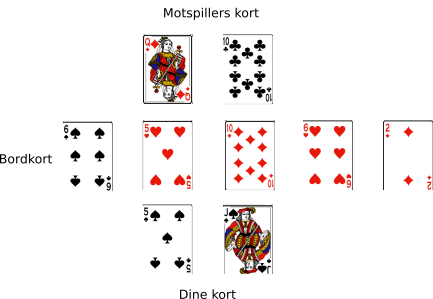
\includegraphics[height=1.5in]{avanserttabbe}
  \captionof*{figure}{Her kan du satse på at motspiller har en dame og ta
	inn femmeren for å så si tabbe dame. Godfølelse å treffe
jackpot!}
  \label{fig:test2}
\end{minipage}
\end{figure}


\begin{figure}[H]
	\centering
	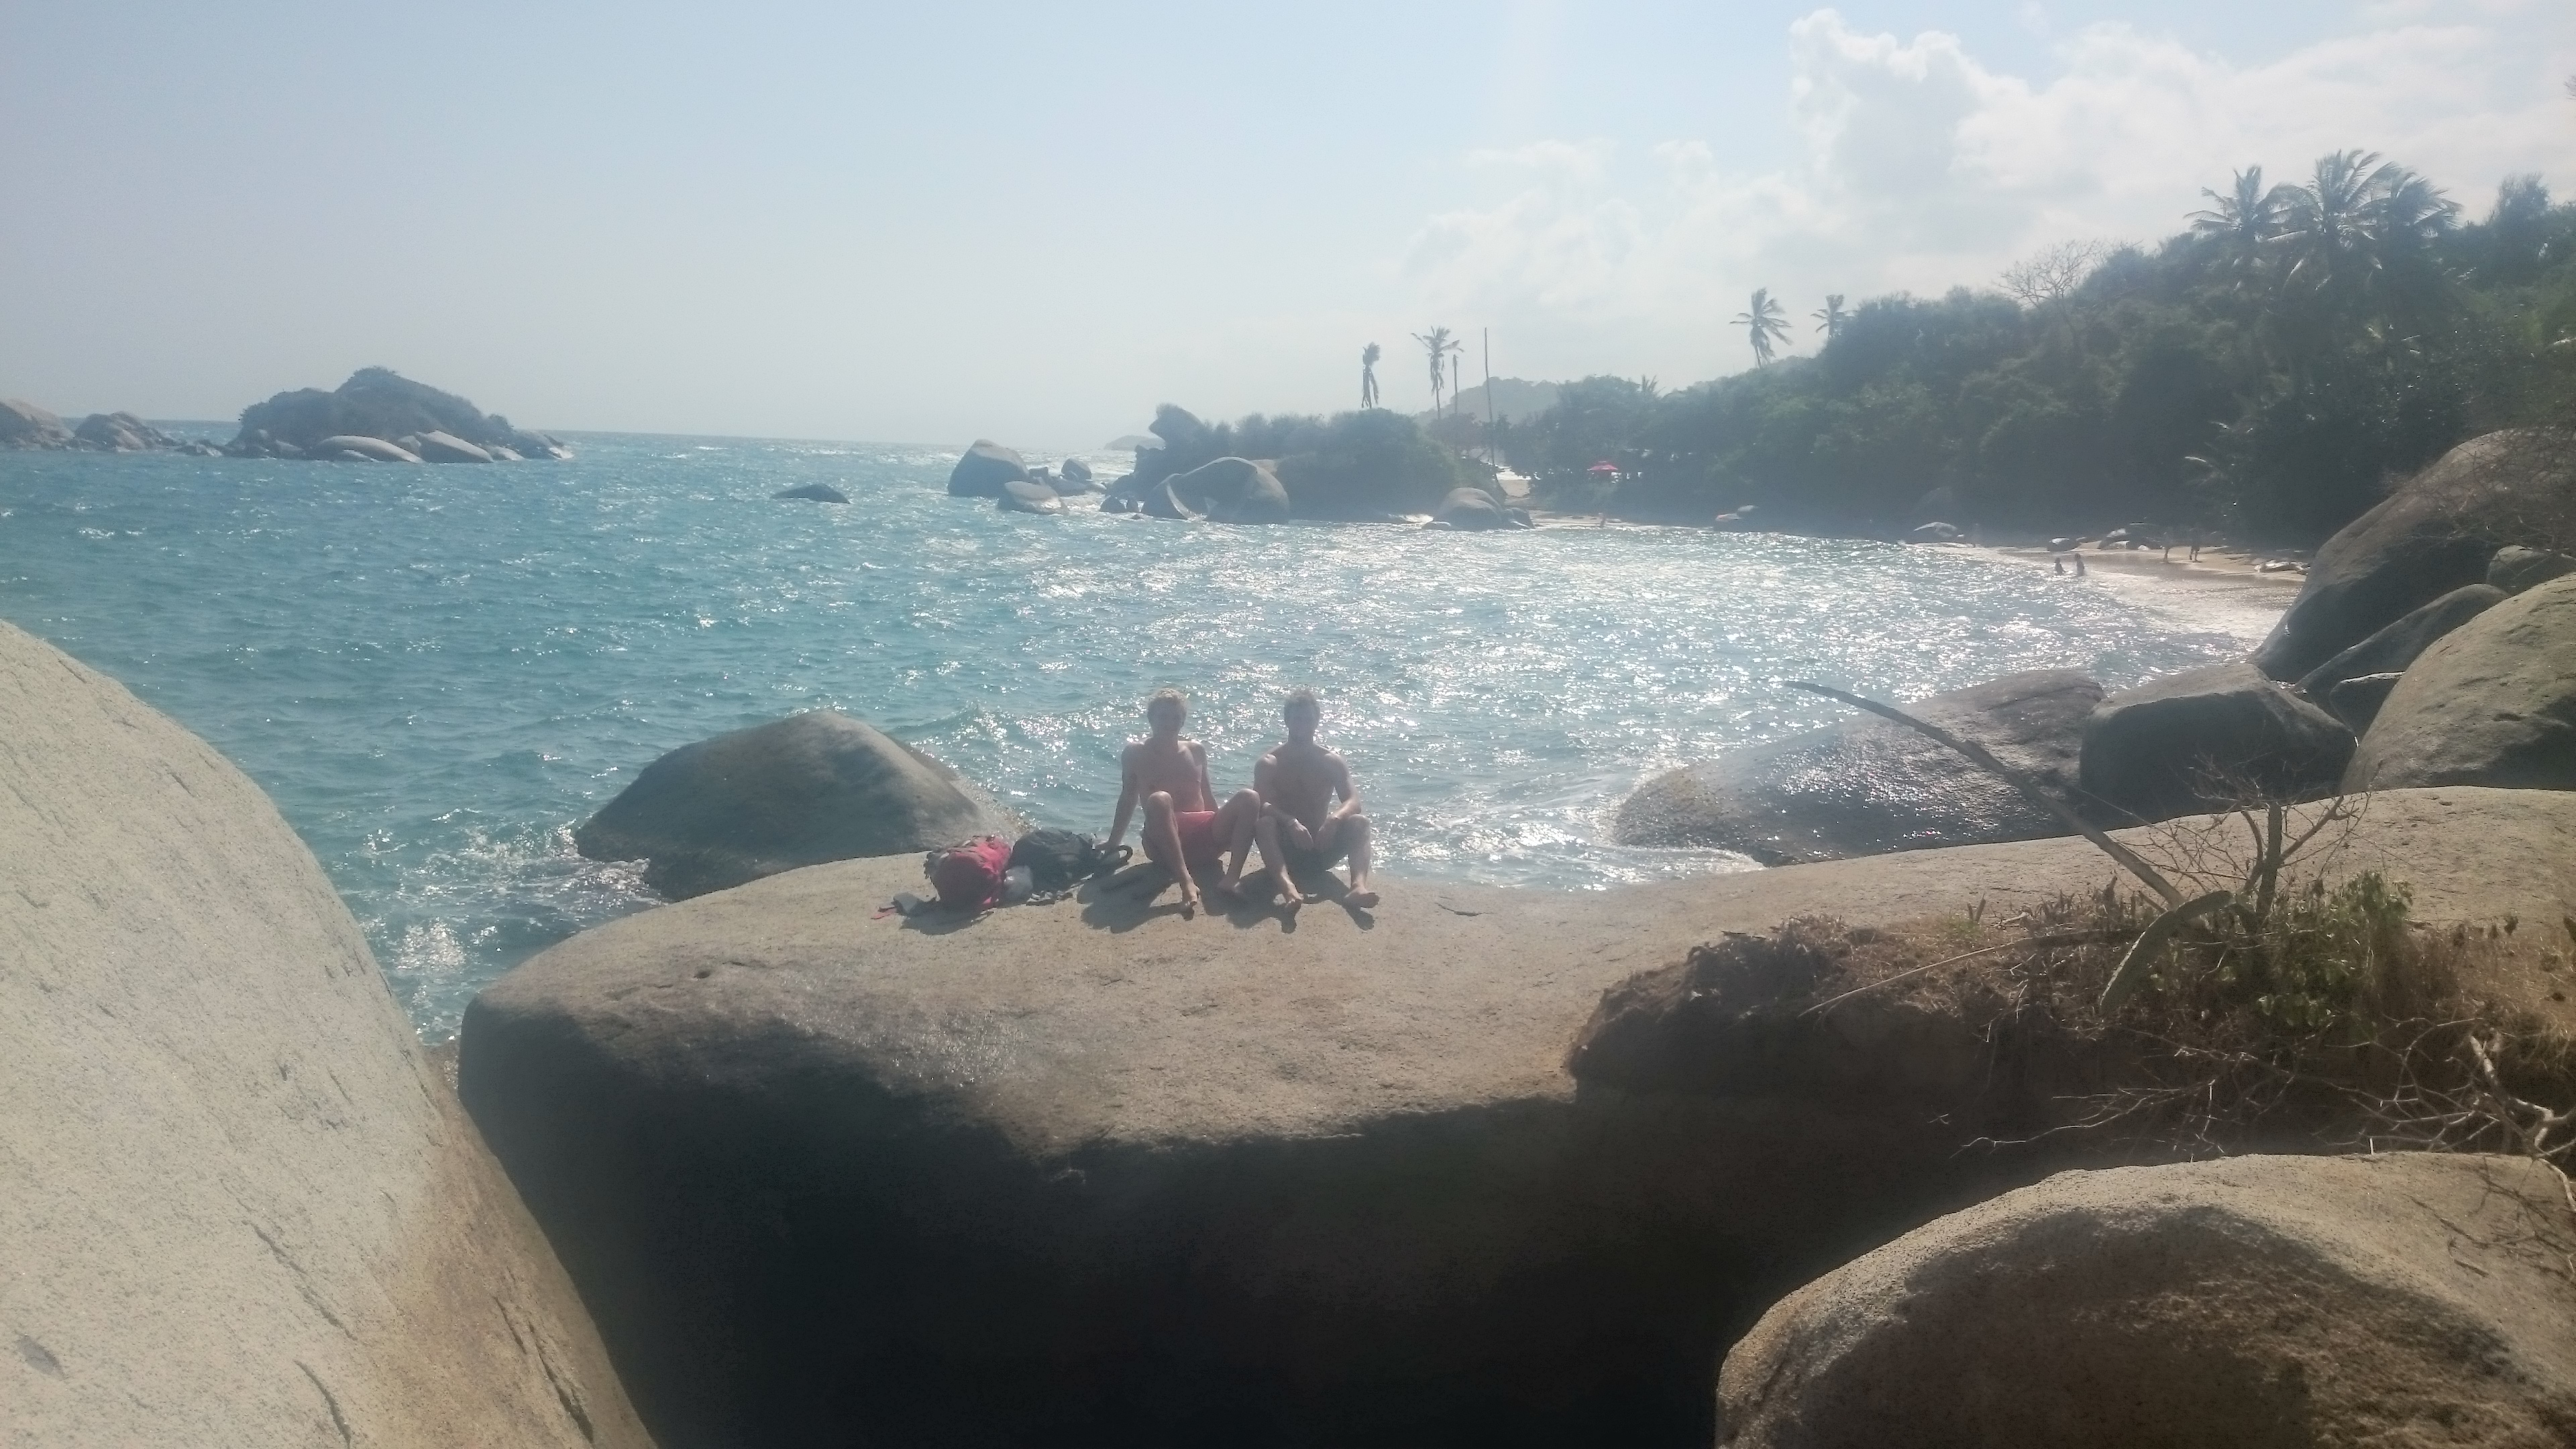
\includegraphics[width=0.7\textwidth]{tayronapark}
	\caption{La janteloven fra oss i Norge og tok en treningsøkt
	her}
	\label{fig:tayronapark}
\end{figure}

\begin{figure}[H]
	\centering
	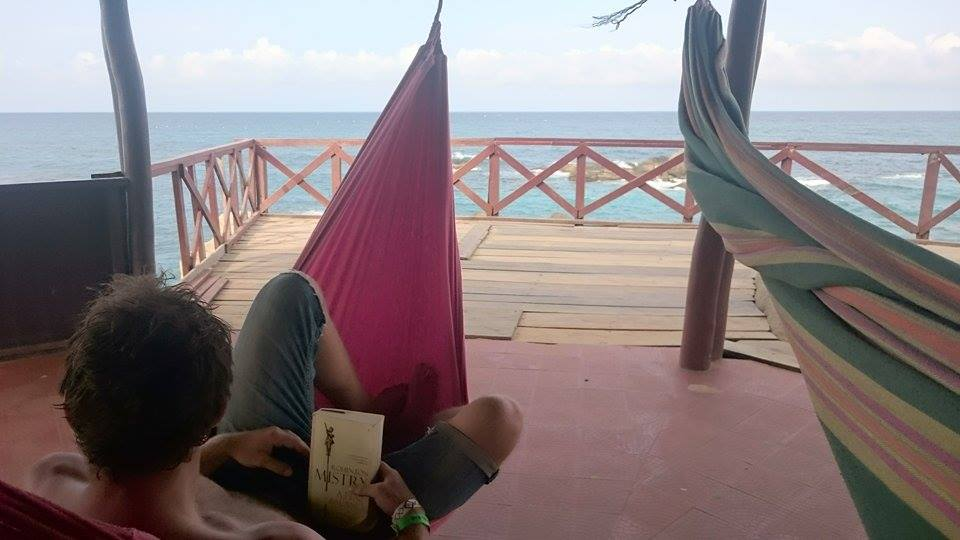
\includegraphics[width=\textwidth]{soveikoye}
	\caption*{Var verd å fryse hele natten da vi så solen stå opp}
	\label{fig:sovekolasj}
\end{figure}

Etter Tayrona stakk vi innom Santa Marta. Vi var egentlig litt slitne
etter dårlig søvn i hengekøyer. Da noen nederlendere inviterte oss med
på en partybuss var det imidlertid vanskelig å si nei. Det er
noe av det kleineste jeg har gjort.. noengang. Forestill deg at du på
er tilbake på russekro. Da inkludert med høy flaskeføring, dunk-dunk
og dansing på en strippestang. Forestill deg nå at denne russekroa er
mobil på en åpen buss. Forestill deg til slutt at du kjører gjennom
sentrum i et land som enda ikke er veldig vant til å se hvite folk.Ikke rart flaskeføringen var
høy\ldots. Jada. Men gøy var det. Mindre gøy neste dag. Da spøy jeg
hver halvtime i 12 timer. Good times. 

\section{Sailoboyz}

Når folk spør meg hva jeg gjorde i Sør-Amerika er svaret: ``Jeg
krysset Andesfjellene, jeg var  Karneval i Rio og jeg seilet fra Colombia
til Panama.'' Disse opplevelsene har en ting til felles. De kan ikke
bli dårlige. Det er ikke mulig. Å seile under den
latinsk-amerikanske solen med en coco-loco i hånden mens man venter på
på neste palmeøy å snorkle rundt kan ikke bli feil. Punktum.

\begin{figure}[H]
	\centering
\noindent\makebox[\textwidth]{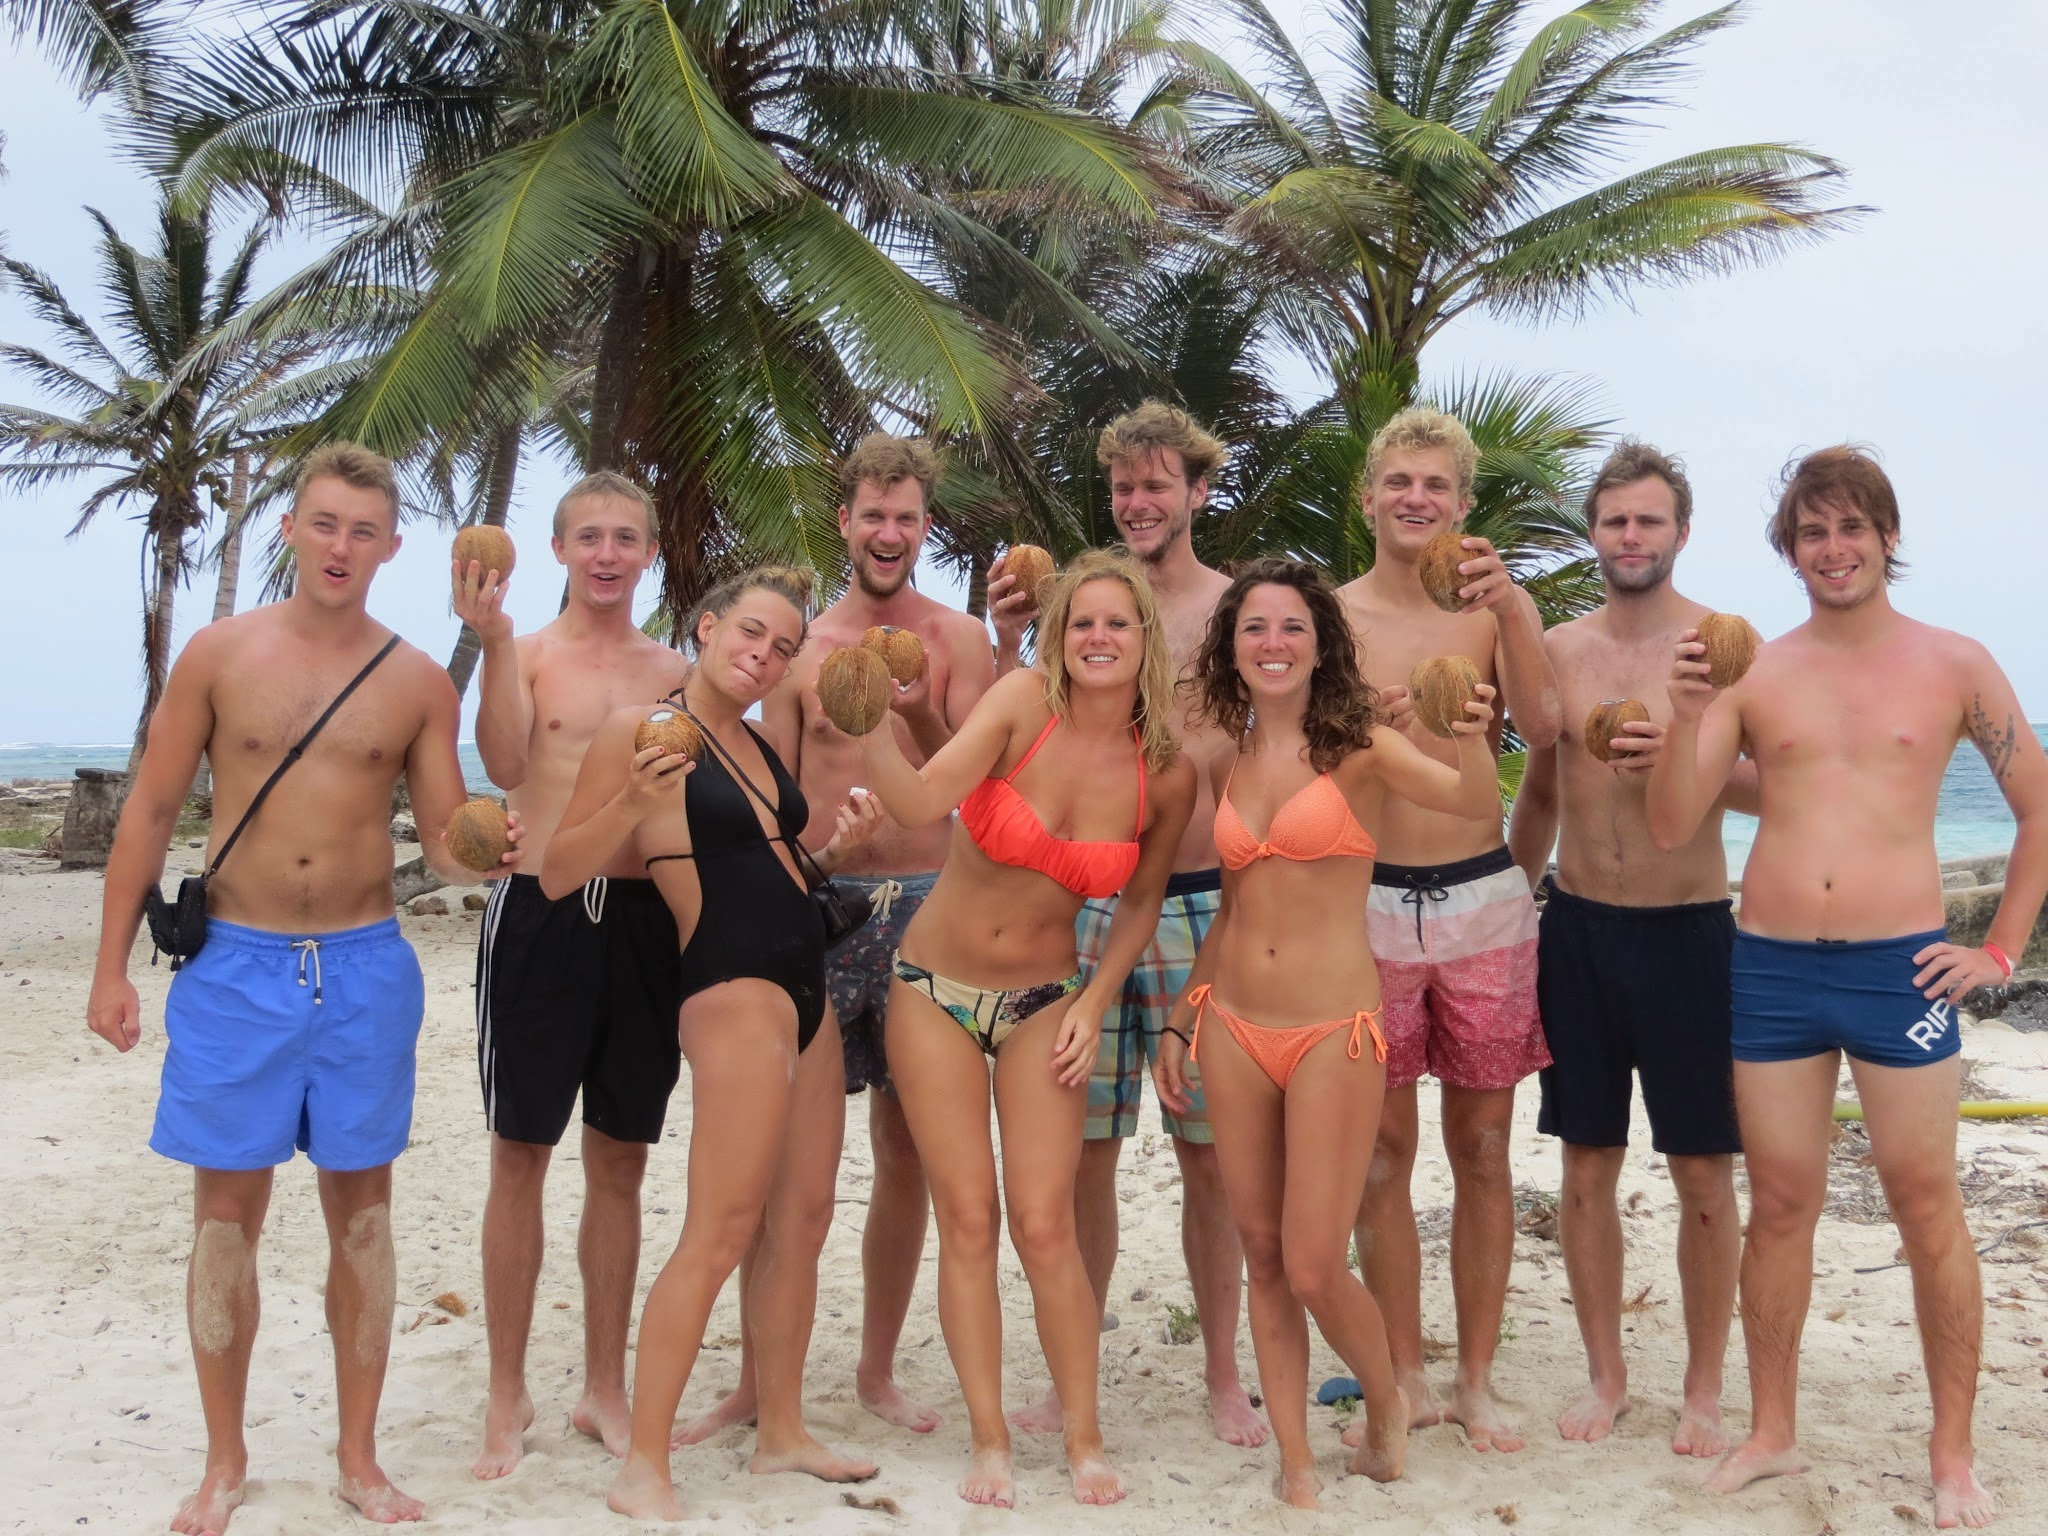
\includegraphics[width=\paperwidth]{minstenotta}}
	\caption{Seilbåtgjengen. Smiler ikke pga jeg fikk den minste
	nøtta}
\label{fig:sanblas}
\end{figure}

\clearpage

\begin{figure}[p]
	\vspace*{-2.7cm}
	\makebox[\linewidth]{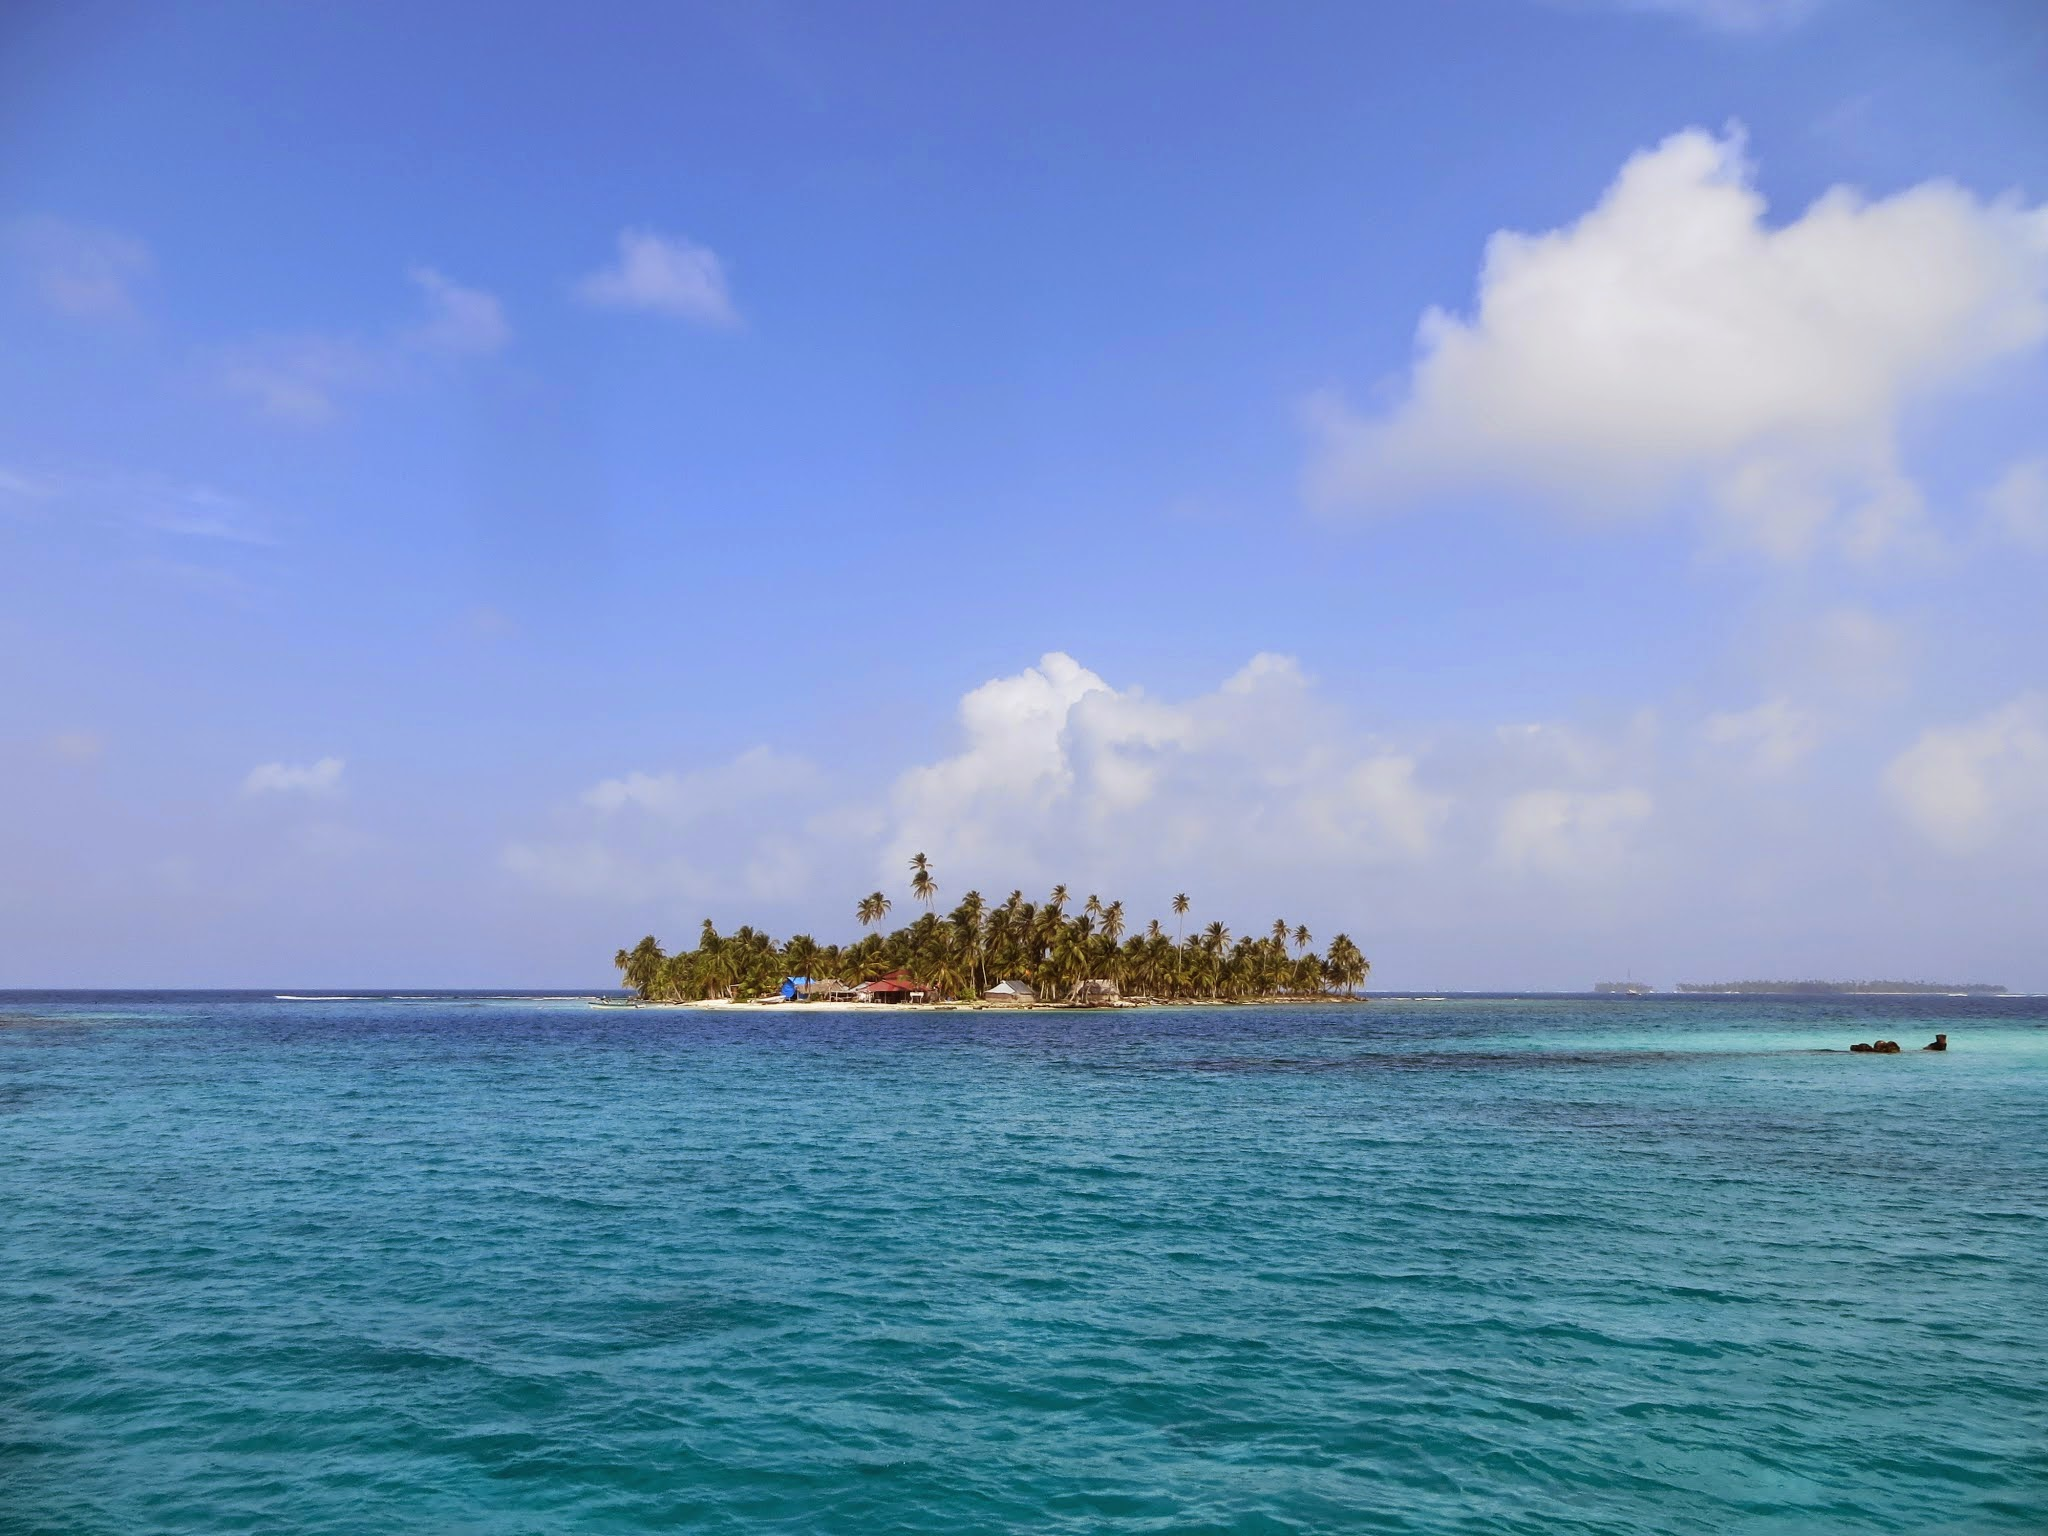
\includegraphics[height=9.3in]{enoy2}}
\end{figure}


%\includepdf{enoy2pdf.pdf\begin{dialogue}


Det som gjorde denne 5 dagers seilasen enda bedre var alle folkene.
Totalt var vi 16 personer. Disse var: 

\begin{itemize}
	\item Clara ei eksentrisk fransk-spanjol som har levd hele
		livet på en løgn
	\item Tom - en brite som har reist i 8mnd etter han slutten i
		bankjobben.
	\item Jente 1 og 2 fra nederland. Derav minst en av dem crusha på Marius
	\item Et nederlandsk par som kunne verdens beste drikkeleker
	\item Blek brite som snorklet en hel dag uten solkrem
	\item En feit sveitser i 30-årene som ikke er over
		trassalderen
\end{itemize}
\begin{figure}[H]
	\centering
	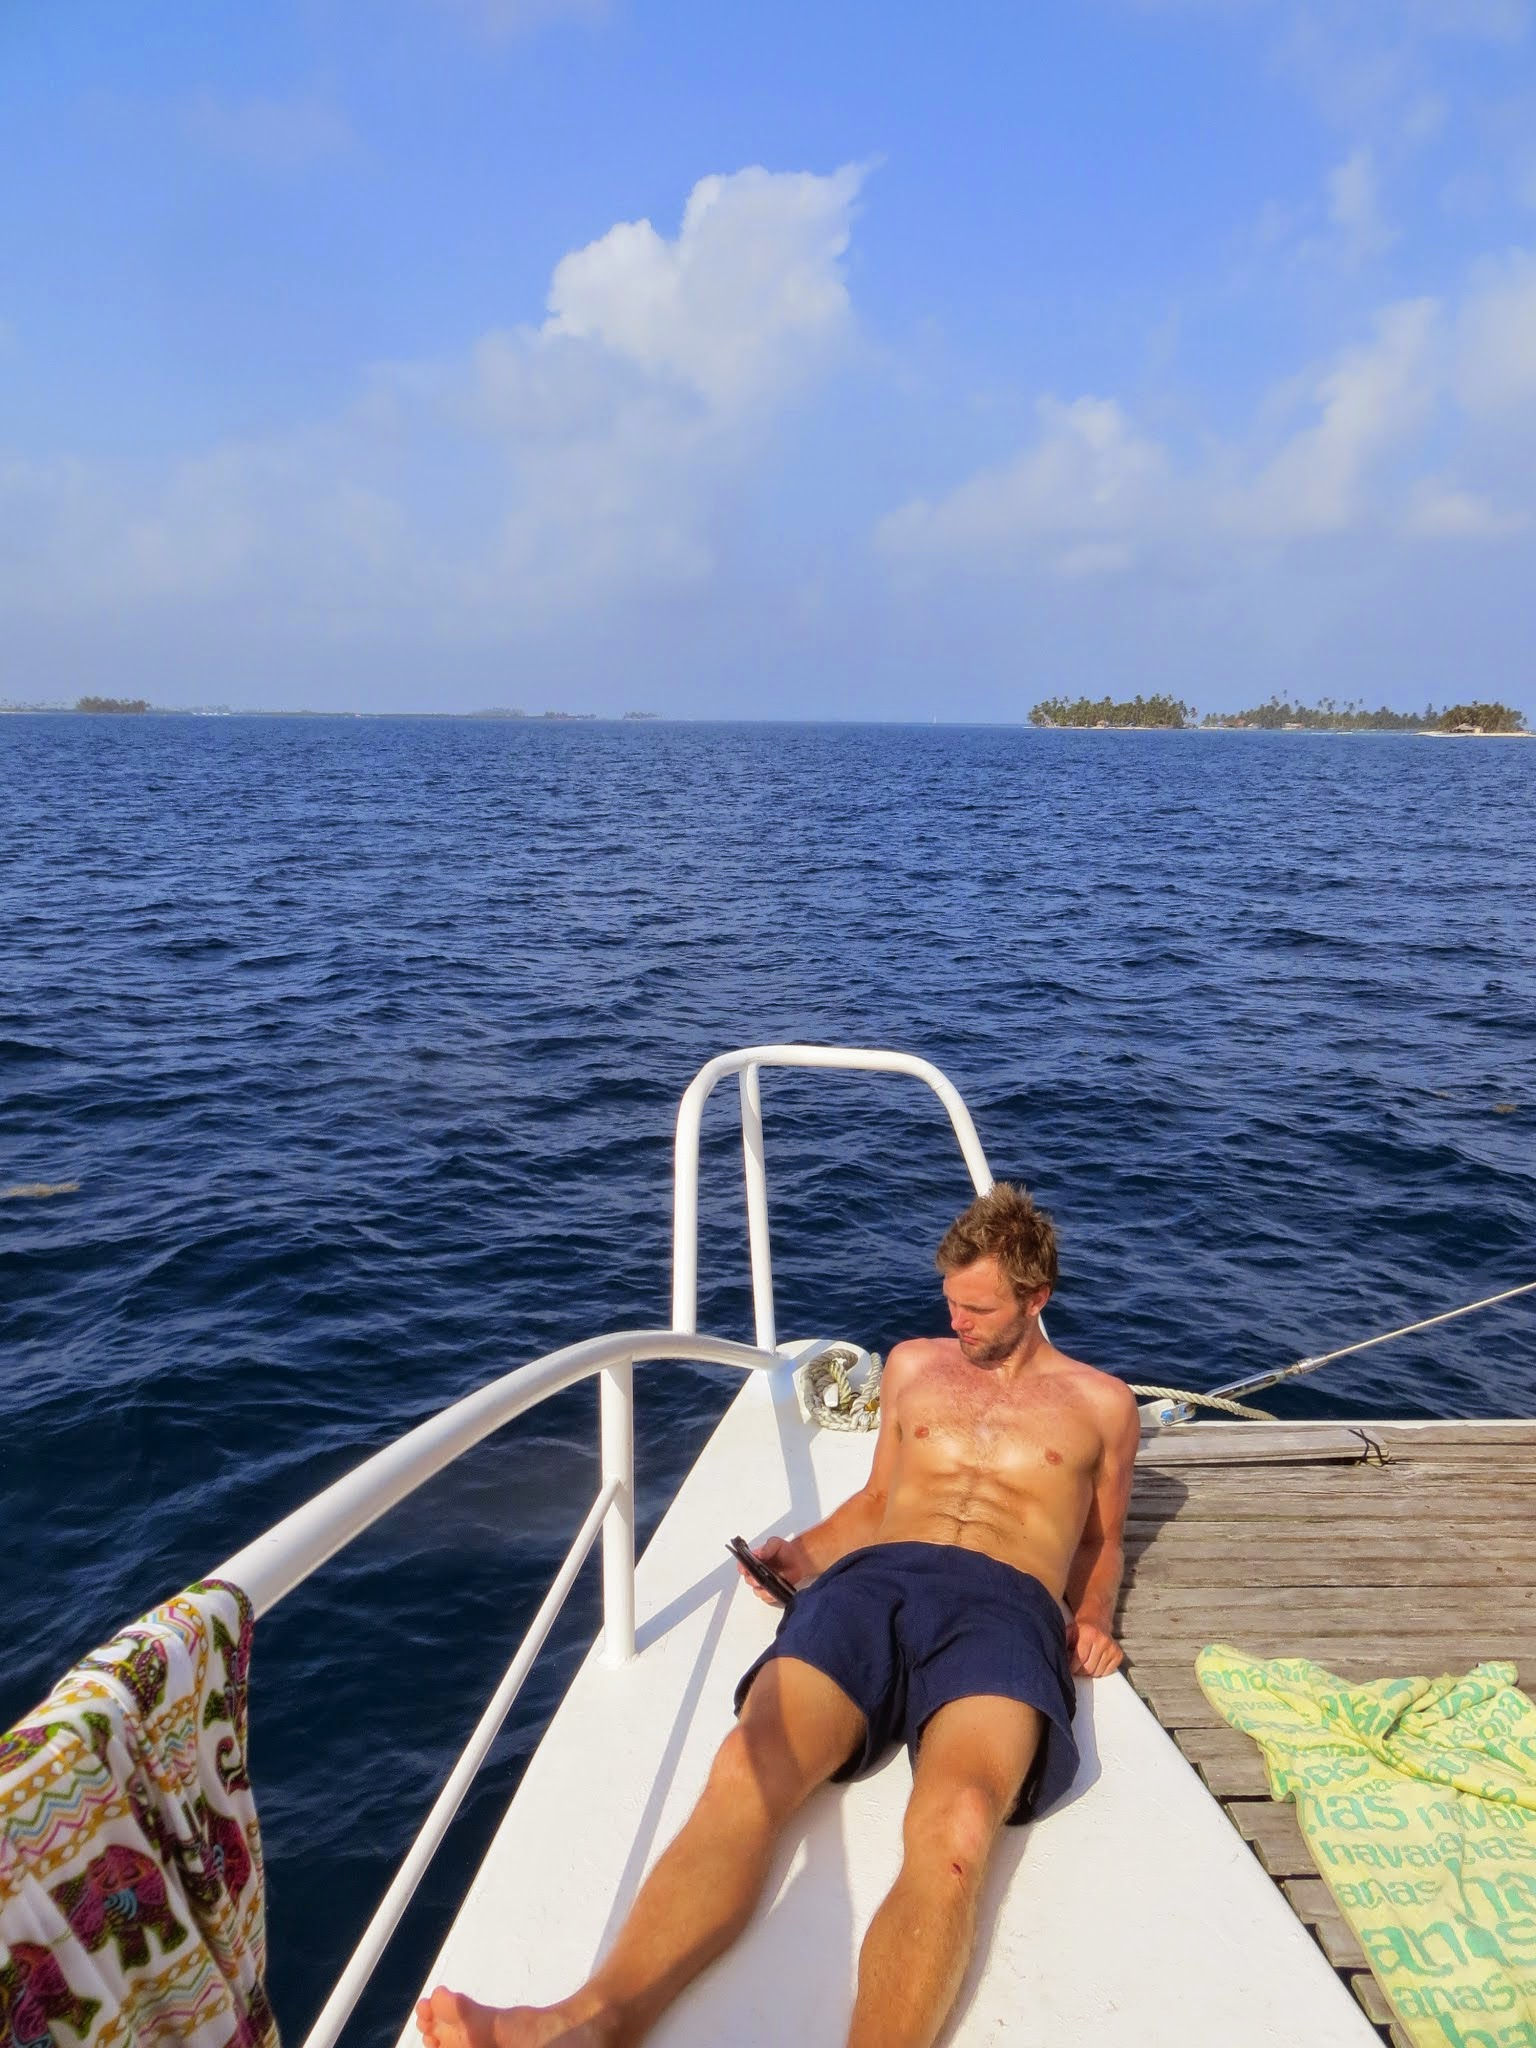
\includegraphics[width=\textwidth]{flex}
	\caption{Ingenting som å ``slappe helt av'' på dekk}
	\label{fig:tintin}
\end{figure}
Seilasen gikk fra Cartagena til øst-siden av Panama. Da over det
Karibiske hav. Først var det 2 døgn på åpent hav. Deretter var det
øyhopping. Dagene fløy forbi mens vi snorklet i det krystallklare vannet
mellom øyer på størrelse med baner.
\begin{figure}[H]
	\centering
	\includegraphics{vollyduel}
	\caption{Nok en konkurranse}
	\label{fig:volley}
\end{figure}


\subsection*{The Norwegian prudes}

Marius og jeg er eventyrlystne karer. Vi er heller ikke fremmede for å
ta oss en fest. Imidlertid er vi nå det kommer til stykke enda
NTNU-avl. Om det ikke er nok at jeg sier det, kan man bare se på
toppturraten og at jeg pakket med meg allværsjakka. Også at jeg
nettopp brukte ordet toppturraten.
Om vi virkelig skulle flippe ut hadde vi kanskje delt en rev.
``fuck-the-system''
Dette syntes noen  på båten var midt mellom søtt og håpløst. Spesielt siden den var prakket av
nederlendere. Europeere utenfor skandinavia har et helt annet syn på narkotika. Eller så
er det mulig vi lever i en boble i Trondheim. Begge deler er nok sant.
Personene på båten var utvilsomt oppegående folk. Hver og en av dem
hadde imidlertid prøvd kokain i løpet av livet. I kontrast kjenner jeg
ikke èn eneste i Trondheim som har prøvd (som jeg vet om).\\

Gateselgere i Colombia gauker om røyk og tyggis før de kommer litt
nærmere å hvisker ``Hashis? Coca?''.  Følgende trodde vi det var
utrolig enkelt å få tak i dop her til lands. Hadde ikke gitt det så
mye tanke, men i mitt naive sinn ville jeg antatt at du bare gjorde
handelen der på stedet. Fort gjort, gjort fort. Dette er historien om
hun som forsøkte:

når ens egen sti er uren. 
er det vanskelig å melde urett som blir begått mot andre og seg selv
\begin{figure}[h]
	\centering
	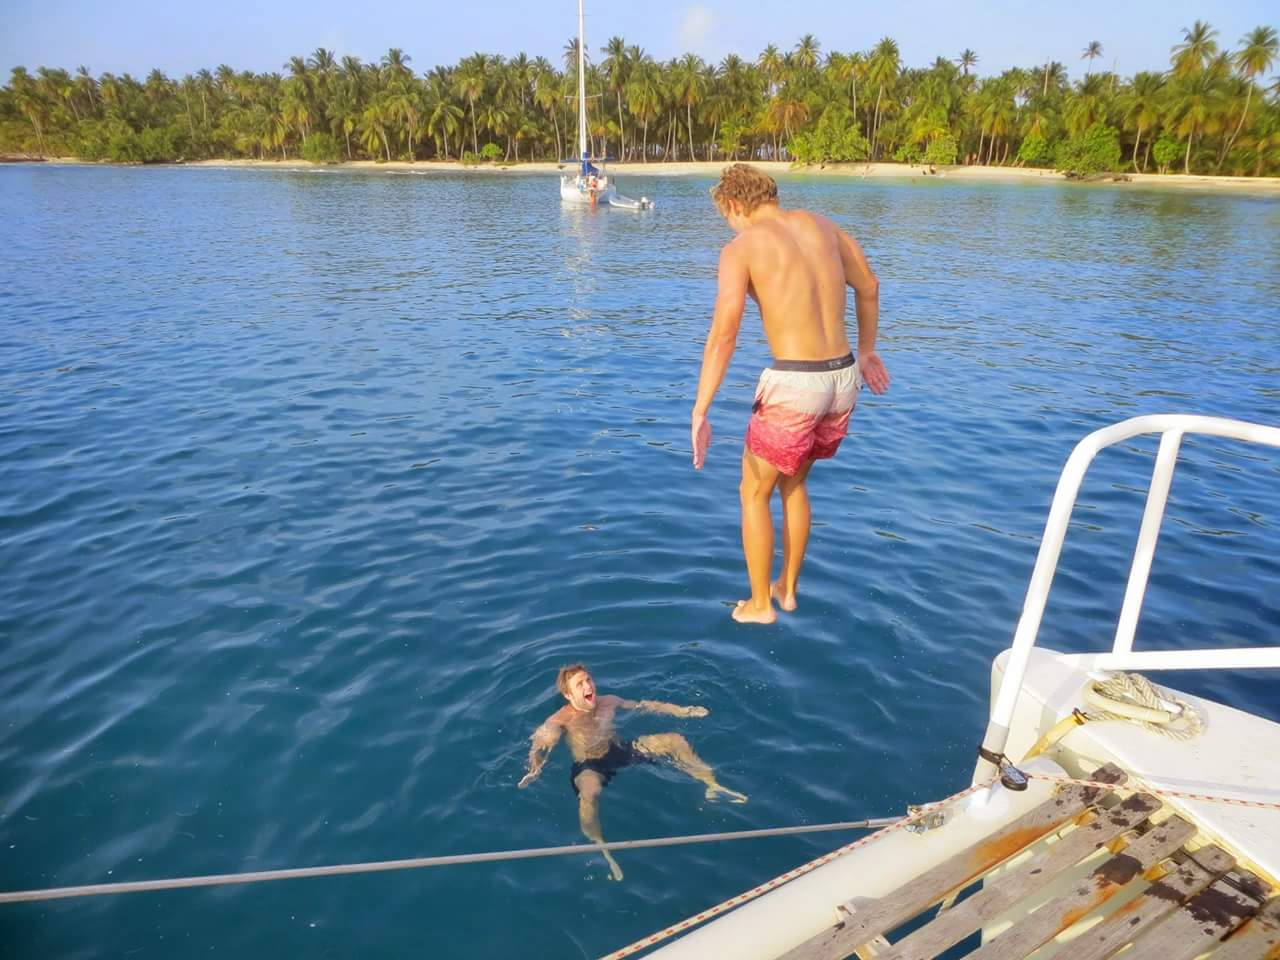
\includegraphics[width=\textwidth]{vennskapvol2}
	\caption{Vennskap vennskap}
	\label{fig:vennskap}
\end{figure}


%Det er mye vanskeligere å melde urett mot en selv når dine egne
%er skitne
%hårklippen i Medillin

\begin{figure}[H]
\twopagepicture{t}{p}{livmaareddes}{}
\end{figure}

\\
\subsection*{My whole life is a lie}

\begin{figure}[H]
	\centering
	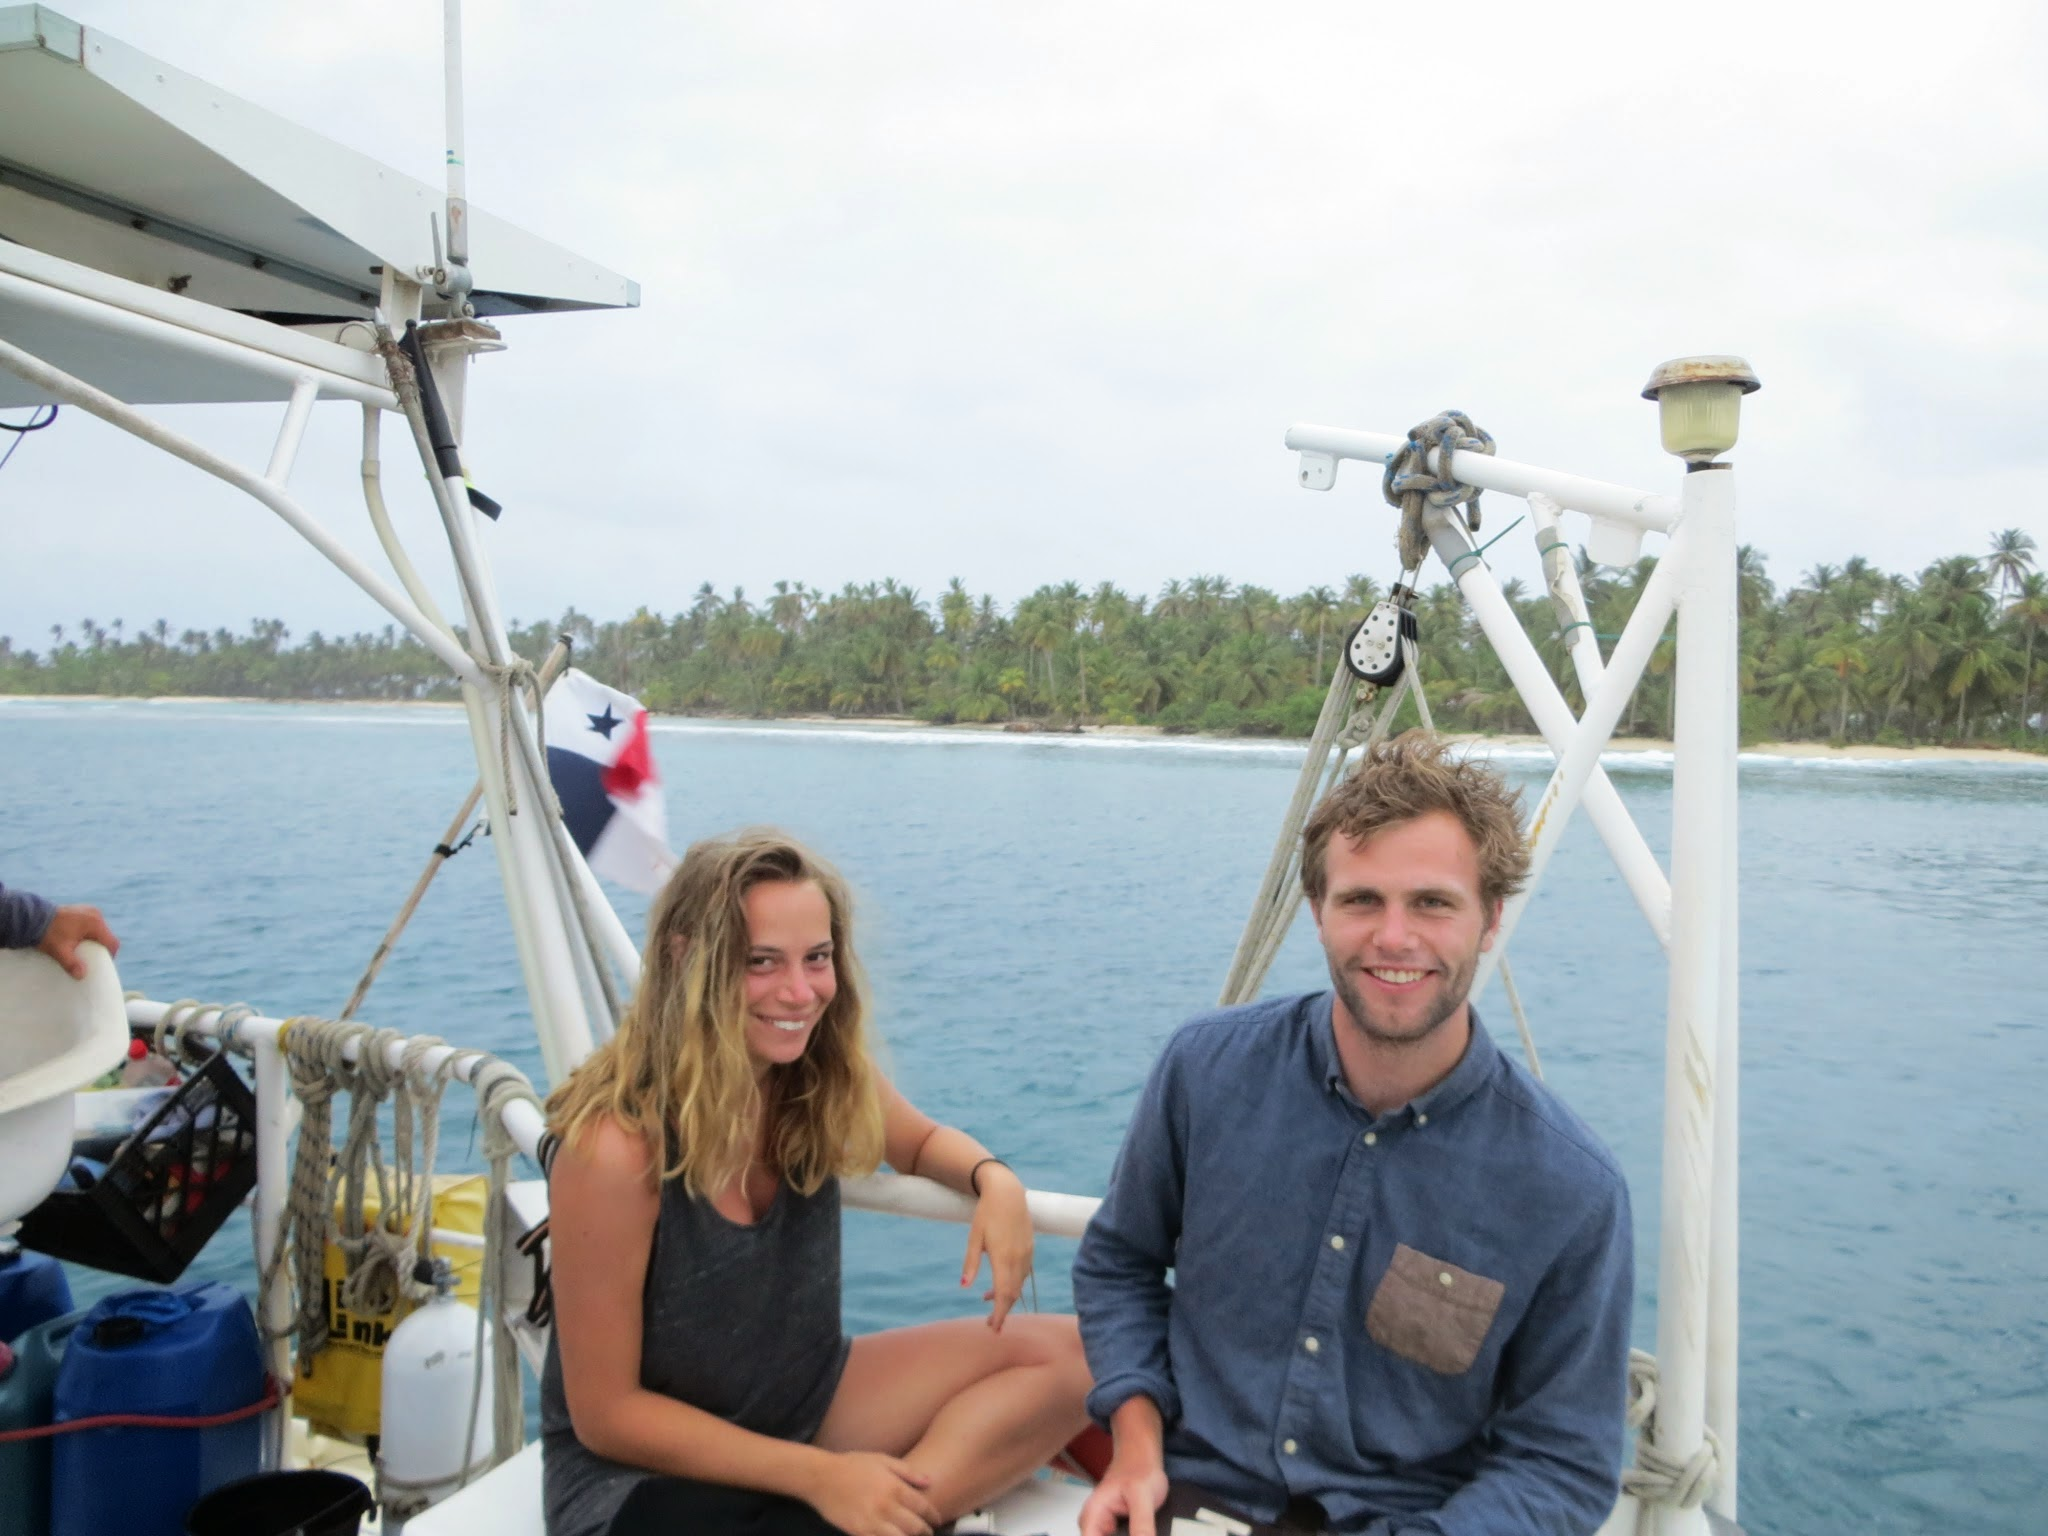
\includegraphics[width=\textwidth]{akselogclara}
	\caption{Clara og Jeg}
	\label{fig:claraogaksel}
\end{figure}

Føttene våre plantes nok en gang på fastlandet. 5 dager har vi vært
til sjøs.  For
noen var det deiligere enn andre. Sveitseren hadde aldri vært i en båt
før. Jevnt over var folket klare for kanakas i Panama-city.
Først måtte vi bare finne et hostel. Det vi ble anbefalt var opptatt.
Det de anbefalte var også opptatt. Lang historie kort: vi endte på det
fjerde på lista. Etter du har reist i Sør-Amerika forstår du at
varmtvann ikke er en selvfølge. imidlertid ville lys i dusje vært greit.
Kvelden gitt som den gikk og Marius, Clara og jeg fikk kapret et
dansegulv så vi slapp sensuell pardans. Marius hoppet stadig opp på
scenen og sang i en mikrofon som lå der. Denne var ikke koblet til
noe. \\
Dagen derpå hadde vi kleinschpiel på en Kafe. Britene lurte på om
det var vanlig med bedè i Norge. Vi svarte med at nordmenn på ferie i
Europa brukte dem til å vaske føttene i.

\begin{dialogue}
	\item Clara: ``Those are not for your feet?''
	\item Tom: ``No, they're for your arse. Instead of
		toiletpaper''
	\item Clara: ``Oh my god, we have one at home, but we use it
		for the feet''
	\item Marius: ``Are you sure that's what the rest of the
		family use it for?''
	\item Clara: ``\ldots''
	\item Clara: ``MY WHOLE LIFE IS A LIE!!''
\end{dialogue}



\section*{Karneval}

\begin{figure}[H]
	\centering

\noindent\makebox[\textwidth]{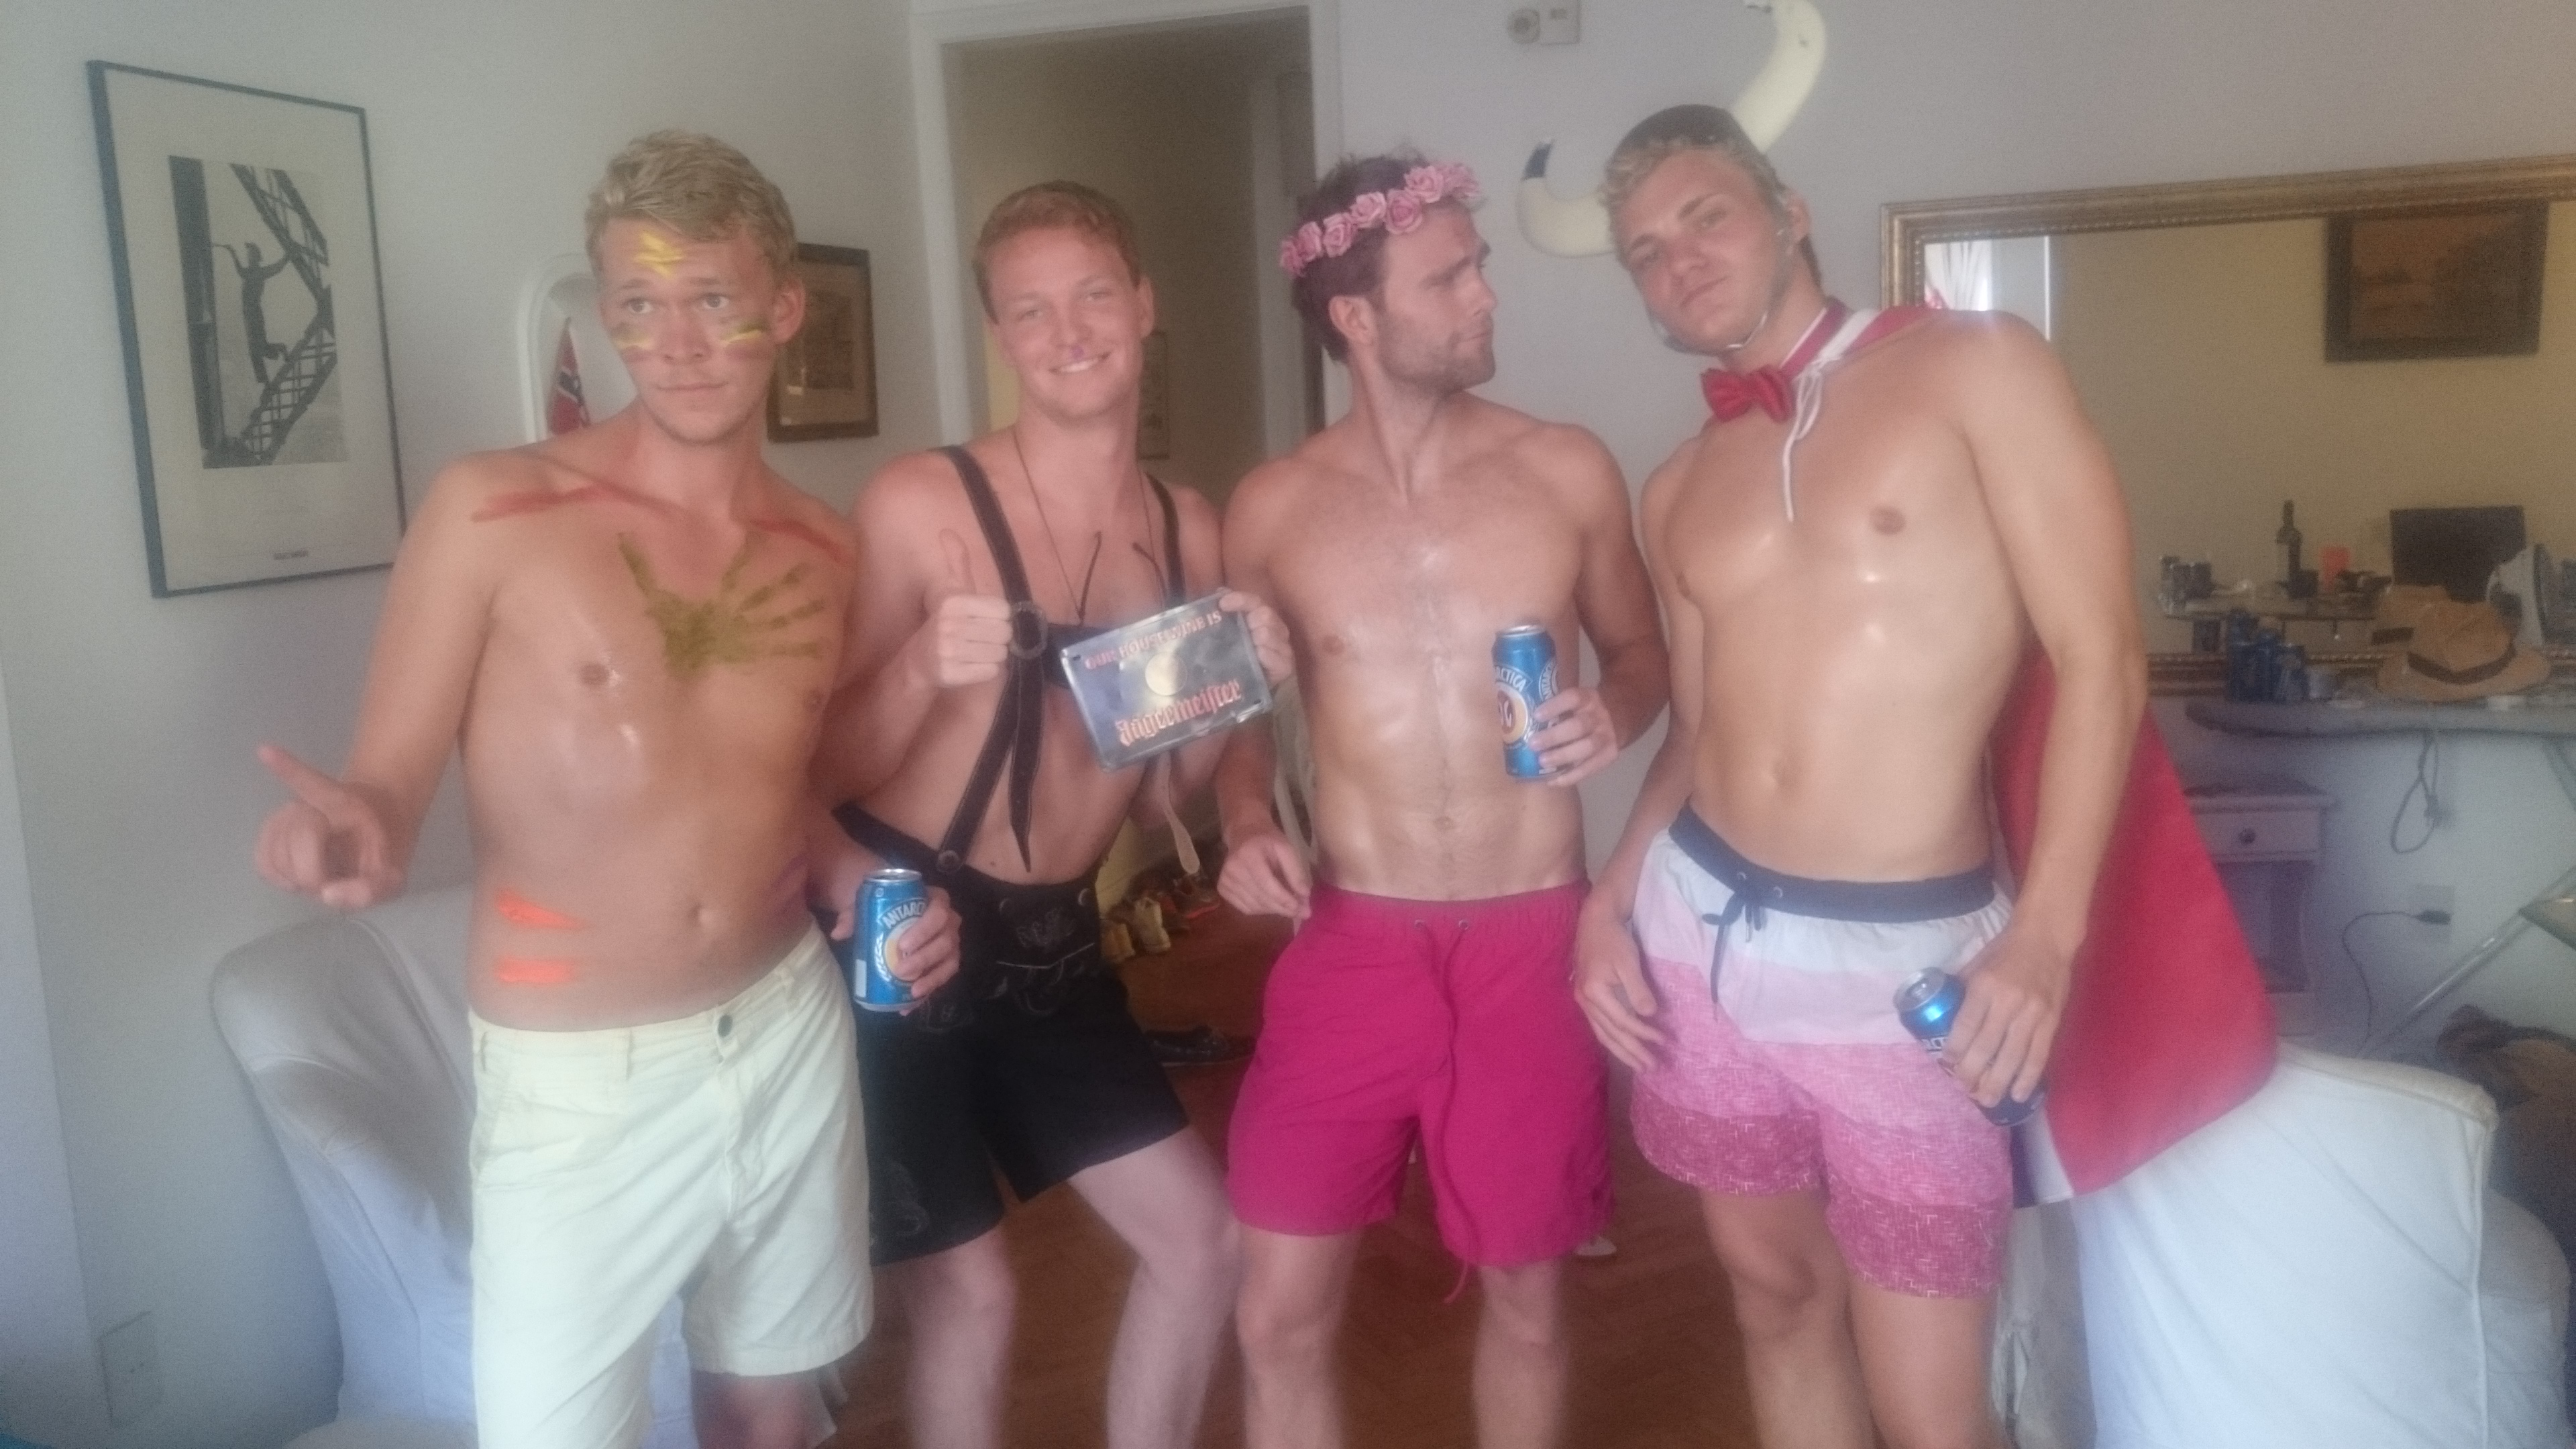
\includegraphics[width=\paperwidth]{homsebloko}}
	\caption{Da vi snublet inn på en homsefest var vi idet minste
	kledd for anledningen}
	\label{fig:homsebloko}
\end{figure}


Vi timet returen og landet i Rio dagen før karneval. I løpet av den
følgende uka ble jeg:

\begin{itemize}
	\item  Gringokongen  etter jeg fikk  en stor gjeng med brasillianere til å falle
		sammen i latter med å vise fargeskille.
	\item Funnet halvveis sovende med hodet inne i kjøleskapet med
		inspirerte matkombinasjoner i hånda
	\item   Uvisst med på homsefest. Da iført bare badebukse, blomsterkrans og et lag med sololje.
	\item Bombadert med kysseforespørslerr mens jeg var utkledd
		som en voksen baby.
	\item Sjarmerende brisen utkledd i matroskostyme med 15 andre
		nordmenn
	\item  Bitt i leggen av to fremmede jenter som stoppet
		med på vei fra do (også utkledd som voksenbaby (jeg
		alså))
	\item Taper av alle beerbongbattles jeg deltok i.
	
\end{itemize}

Alle disse punktene har en historie. De vil imidlertid bli tatt
muntlig og sensurert avhengig av lytter. Så bare å spørre!
